\documentclass[12pt,oneside]{memoir}

% \usepackage[utf8]{inputenc}
\usepackage{cmsrb}
\usepackage{listings}
\usepackage{matfmaster}
\usepackage{url}
\usepackage{graphicx}
\usepackage{float}
\usepackage{hyperref}
\usepackage{caption}
\usepackage{ragged2e}

\usepackage{color}
\definecolor{lightgray}{rgb}{.9,.9,.9}
\definecolor{darkgray}{rgb}{.4,.4,.4}
\definecolor{purple}{rgb}{0.65, 0.12, 0.82}
\definecolor{customGreen}{rgb}{0.25, 0.85, 0.25}

\lstdefinelanguage{Swift}{
  keywords={associatedtype, class, deinit, enum, extension, fileprivate, func, import, init, inout, internal, let, open, operator, private, precedencegroup, protocol, public, rethrows, static, struct, subscript, typealias, var, break, case, catch, continue, default, defer, do, else, fallthrough, for, guard, if, in, by, repeat, return, throw, switch, where, while, Any, as, catch, false, is, nil, rethrows, self, Self, super, throw, throws, true, try, _, associativity, convenience, didSet, dynamic, final, get, indirect, infix, lazy, left, mutating, none, nonmutating, optional, override, postfix, precedence, prefix, Protocol, required, right, set, some, Type, unowned, weak, willSet, @State, List, View, Image, VStack, Text, color, action},
  keywordstyle=\color{blue}\bfseries,
  ndkeywords={Int, String, Double, Float, Bool},
  ndkeywordstyle=\color{customGreen}\bfseries,
  identifierstyle=\color{black},
  sensitive=false,
  comment=[l]{//},
  morecomment=[s]{/*}{*/},
  commentstyle=\color{purple}\ttfamily,
  stringstyle=\color{orange}\ttfamily,
  morestring=[b]',
  morestring=[b]"
}

\lstset{
   language=Swift,
%   backgroundcolor=\color{datgray},
   extendedchars=true,
   basicstyle=\footnotesize\ttfamily,
   showstringspaces=false,
   showspaces=false,
   numbers=left,
   numberstyle=\footnotesize,
   numbersep=9pt,
   tabsize=4,
   breaklines=true,
   showtabs=false,
   captionpos=b
}

\bib{literatura}

\autor{Марко Вељковић}
\naslov{Креирање виџета у програмском језику Swift}
\godina{2022}
\mentor{др Милена \textsc{Вујошевић Јаничић}, ванредни професор\\ Универзитет у Београду, Математички факултет}
\komisijaA{др Филип \textsc{Марић}, ванредни професор\\ Универзитет у Београду, Математички факултет}
\komisijaB{др Мирко \textsc{Спасић}, доцент\\ Универзитет у Београду, Математички факултет}
\datumodbrane{јун 2022.}

\apstr{
Програмски језик \textit{Swift} се користи приликом израде апликација намењених платформама компаније \textit{Apple}. Виџет је део апликације који приказује одабране важне информације на почетном екрану уређаја. Да би се развио виџет потребна је употреба радног окружења \textit{SwiftUI} које користи декларативну синтаксу. Циљ рада је представљање основних особина и карактеристика програмског језика \textit{Swift} и приказ развоја виџета употребом радног окружења \textit{SwiftUI}. Развијена је апликација "Кулинарство --- сласно и ефикасно" која представља конкретан пример употребе програмског језика \textit{Swift} приликом развоја апликације за оперативни систем \textit{iOS}. Поред апликације приказано је и креирање виџета који је развијен у склопу ове апликације.  
}

\kljucnereci{програмски језици, развој софтвера, \textit{Apple}, \textit{iOS}, \textit{Swift}, виџети}

\renewcommand\lstlistingname{Пример кода}
%\renewcommand\lstlistlistingname{Algorithms}

\begin{document}

\frontmatter
\naslovna

\chapter*{}
\thispagestyle{empty}
\begin{flushright}
\Large{\textit{Мојој породици и пријатељима на подршци и менторки на помоћи и саветима}}
\end{flushright}

\komisija
\apstrakt
\tableofcontents*

\mainmatter

\chapter{Увод}

\indent \textit{Swift} jе модеран програмски jезик опште намене, настао 2014. године у оквиру компаниjе \textit{Apple}. Првенствено jе намењен развоjу апликациjа на њиховим платформама (\textit{iOS}, \textit{iPadOS}, \textit{macOS}, \textit{tvOS} и \textit{watchOS}), али jе део развоjа jезика усмерен ка поjедностављивању процеса израде корисничког интерфеjса и увођењу декларативне синтаксе у jезик. У том контексту настало jе радно окружење (енг. \textit{framework}) \textit{SwiftUI} коjе одликуjе могућност брзог креирања концизних и ефикасних решења. Пример примене радног окружења \textit{SwiftUI} jе израда виџета намењених оперативним системима \textit{iOS}, \textit{iPadOS} и \textit{macOS}. 
\\
\indent Виџет, као део мобилне апликациjе, се налази на почетном екрану уређаjа (телефона или таблета) и кориснику приказуjе одабране важне информациjе из те апликациjе. За разлику од виџета у оперативном систему \textit{Android}, коjи су присутни више од десет година, виџети на платформама компаније \textit{Apple} су уведени 2020. године, тако да jе и сама технологиjа коjа подржава њихово креирање и даље у активном развоjу.
\\
\indent Циљ рада jе истраживање и опис карактеристика и могућности коjе пружа програмски jезик \textit{Swift}, промене и побољшања коjе jе донело радно окружење \textit{SwiftUI} и приказ новина насталих увођењем виџета (конкретно у оперативном систему \textit{iOS}). У оквиру рада је имплементирана \textit{iOS} апликациjа о кулинарству "Кулинарство --- сласно и ефикасно" коришћењем програмског jезика \textit{Swift}, након чега је креиран одговараjући виџет помоћу радног окружења \textit{SwiftUI}. Оваj виџет пружа кориснику помоћ приликом избора и припреме оброка.
\\
\indent У глави 2 представљен је програмски језик \textit{Swift}, описане су његове карактеристике, основни и напредни концепти, и особине које одликују овај програмски језик. Описано је интегрисано развојно окружење (ИРО) \textit{Xcode} у којем се развијају апликације намењене платформама компаније \textit{Apple}, као и радно окружење \textit{SwiftUI}. Глава 3 описује виџет као део мобилне апликације у оперативном систему \textit{iOS}, развој виџета, као и правила и препоруке приликом његовог дизајнирања. У глави 4 представљена је имплементација и визуелни приказ апликације "Кулинарство --- сласно и ефикасно", и виџета који је креиран уз апликацију. Последња, 5. глава представља закључак целокупног рада и приказује даља унапређења апликације.

\chapter{Програмски језик \textit{Swift}}

\indent \textit{Swift} је модеран програмски језик настао као резултат истоименог пројекта унутар компаније \textit{Apple}, чији је циљ био креирање програмског језика  који ће бити сигуран, концизан и ефикасан. Резултати пројекта \textit{Swift} као и унапређења програмског језика \textit{Swift} током година биће приказани у наставку. 

\section{Настанак, развој и карактеристике}

\indent Развој програмског језика \textit{Swift} започео је Крис Латнер\footnote{Софтверски инжењер најпознатији по развоју технологија \textit{LLVM}, компајлера \textit{Clang} и програмског језика \textit{Swift}.} (енг. \textit{Chris Lattner}) у јулу 2010. године. У јуну 2014. године објављена је прва апликација комплетно написана у \textit{Swift}-у названа \textit{"Apple Worldwide Developers Conference"} (\textit{WWDC}) по истоименој годишњој конференцији информационих технологија компаније \textit{Apple}. На конференцији те године, кроз предавање и интерактивну демонстрацију, представљена је бета верзија језика, бесплатна књига "The Swift Programming Language" \cite{The_Swift_Programming_Language} и званична веб страница програмског језика \cite{SwiftOfficialSite}. Прва званична верзија језика \textit{Swift} 1.0, постала је доступна 9. септембра 2014. године.

\indent Званично објављивање апликација (на \textit{App Storе}-у) писаних у \textit{Swift}-у постало је могуће од верзије програмског језика 2.0. Језик је у оквиру анкете коју организује  \textit{Stack Overflow}  \cite{StackOverflow} проглашен за омиљени програмски језик 2015. године, док је 2016. године заузео друго место у тој категорији. Децембра 2015. године изворни к\^{o}д језика, подржане библиотеке, дибагер и менаџер пакета постали су отвореног кода, под лиценцом \textit{Apache} 2.0, доступни на \textit{GitHub}-у \cite{GitHub_Swift}.

\indent На годишњој конференцији \textit{WWDC} 2016. године представљена је апликација за уређај \textit{iPad} под називом \textit{Swift Playgrounds} \cite{Swift_Playground}, која је намењена учењу програмирања у \textit{Swift}-у. Касније је ова апликација развијена и за оперативни систем \textit{macOS}.

\indent Током конференције 2019. године представљено је радно окружење \textit{SwiftUI} \cite{Swift_SwiftUI} које омогућава декларативно програмирање апликација за све платформе компаније \textit{Apple}. У време писања рада последња званична верзија језика је \textit{Swift} 5.6.

\begin{figure}[H]

\includegraphics[width=0.5\textwidth]{images/Swift_logo.png}
\centering
\caption{\textit{Swift лого}}
\label{slika:swift_logo}
\end{figure}

\indent \textit{Swift} је моћан и интуитиван језик за програмирање апликација намењених платформама компаније \textit{Apple}. Писање кода у \textit{Swift}-у је забавно и лако, синтакса је веома концизна, али у исто време веома изражајна. Програмски језик \textit{Swift} је безбедан, брз и интерактиван, и као такав погодан за људе који уче основе програмирања. К\^{o}д писан у \textit{Swift}-у се преводи и оптимизује тако да извуче максимум из хардверских компоненти. Детаљнији опис особина и примери кодирања биће дати у наредним поглављима. 

\section{Основни концепти језика}
\label{sec:Концепти}

\indent \textit{Swift} је наследник програмских језика \textit{C} и \textit{Obјective-C}, па је самим тим одређенe концептe преузео из ових језика, али истовремено постоје концепти у \textit{Swift}-у који нису присутни у \textit{C}-у и \textit{Obјective-C}-у. Објашњење најбитнијих концепата у \textit{Swift}-у дато је у наставку, док се потпуна листа може наћи на званичном сајту програмског језика \cite{SwiftOfficialSite}.

\subsection{Основе програмског језика \textit{Swift}}

\indent \textit{Swift} подржава основне типове променљивих, \textit{Int} за целобројне вредности, \textit{Float} и \textit{Double} за бројеве са основом у покретном зарезу, \textit{Bool} за Булове вредности, \textit{String} за текстуалне вредности, као и три основна типа колекција \textit{Array}, \textit{Set} и \textit{Dictionary} о којима ће бити више речи у делу \ref{subsec:Колекције} --- \nameref{subsec:Колекције}. 
\\ 
\indent Поред основних типова који су наслеђени из \textit{Objective-C}-а постоје и неколико ново уведених, као што је \textit{Tuples} (торка) који омогућава креирање груписаних вредности и \textit{Optionals} помоћу којег се рукује \textit{nil} вредношћу на безбедан начин.
\\
\indent Константе се декларишу коришћењем кључне речи \textit{let}, након чега следи име константе и њена иницијализација. Декларисање променљиве се постиже употребом кључне речи \textit{var}. Када се декларише променљива може се одмах и иницијализовати или јој може бити додељен тип употребом анотације. Конкретна примена се може видети у примеру \ref{lst:Декларисање променљивих и константи} --- \nameref{lst:Декларисање променљивих и константи}.

\begin{lstlisting}[caption=\textit{Декларисање променљивих и константи}, label={lst:Декларисање променљивих и константи}, language=Swift, frame=single]
// Deklarisanje konstante
let cenaJela = 200

// Deklarisanje promenljive uz inicijalizaciju
var raspolozivoNovca = 1000

// Deklarisanje promenljive koriscenjem anotacije
var brojPorcija: Int
\end{lstlisting}

\indent Целобројне променљиве могу бити написане у облику децималних, бинарних, окталних и хексадецималних бројева. Пример дефинисања променљиве са вредношћу броја 25 у свим облицима следи у наставку \ref{lst:Целобројне променљиве} --- \nameref{lst:Целобројне променљиве}.

\begin{lstlisting}[caption=\textit{{Целобројне променљиве}}, label={lst:Целобројне променљиве}, language=Swift, frame=single]
var mojiBroj = 25 
var binarniBroj = 0b11001     // 25 u binarnom obliku
var oktalniBroj = 0o31        // 25 u oktalnom obliku
var heksadecimalniBroj = 0x19 // 25 u heksadecimalnom obliku
\end{lstlisting}

\indent Торка се користи за груписање вредности било ког типа и једна торка може садржати вредности различитих типова. У примеру \ref{lst:Торка} --- \nameref{lst:Торка} могу се видети два начина креирања торке и два начина приступања члановима торке (неименованим и именованим члановима).

\begin{lstlisting}[caption=\textit{{Торка}}, label={lst:Торка}, language=Swift, frame=single]
// Definisanje torke (String, Int)
let namirnicaSaCenom = ("Jaja 10 komada", 100)

// Pristupanje clanovima torke
let namirnica = namirnicaSaCenom.0
let cena = namirnicaSaCenom.1

// Definisanje torke sa imenovanim clanovima
let urednijaNamirnicaSaCenom = (namirnica: "Jaja 10 komada", cena: 100)

// Pristupanje imenovanim clanovima torke
let urednijaNamirnica = urednijaNamirnicaSaCenom.namirnica
let urednijaCena = urednijaNamirnicaSaCenom.cena
\end{lstlisting}

\indent Провере испуњености услова коришћењем функције \textit{assert} се дешавају у време извршавања кода. Најчешће се користи за проверу критичног дела кода и уколико тај део кода задовољава услов (вредност израза у \textit{assert}-у је \textit{true}) програм наставља своје извршавање. У супротном извршавање апликације ће бити прекинуто и биће означено место у коду у коме је дошло до прекида програма. Пример примене је приказан у коду \ref{lst:Провере коришћењем функције assert} --- \nameref{lst:Провере коришћењем функције assert}.

\begin{lstlisting}[caption=\textit{{Провере коришћењем функције assert}}, label={lst:Провере коришћењем функције assert}, language=Swift, frame=single]
var cenaPrvogProizvoda = 100
var cenaDrugogProizvoda = -100
assert(cenaPrvogProizvoda >= 0, "Cena proizvoda ne moze biti negativna") //true
assert(cenaDrugogProizvoda >= 0, "Cena proizvoda ne moze biti negativna") //false
\end{lstlisting}

\subsection{Оператори}

\indent Као и у већини програмских језика, постоје три основне врсте оператора: 

\begin{itemize}
  \item Унарни оператори
  
\begin{itemize}
    \item префиксни унарни оператори (на пример, '-' за бројевне вредности и '!' за логичке вредности),  
    \item постфиксни унарни оператори (на пример, '?' и '!' који се користе над опционим променљивима).
\end{itemize}
  
  \item Бинарни оператори
  
\begin{itemize}
    \item оператор доделе '=', који за разлику од језика C, не враћа повратну вредност,
    \item аритметички оператори, '+', '-', '*', '/', '\%',
    \item сложени оператори доделе, '+=', '-=', '*=', '/=',
    \item оператори поређења, '==', '!=', '<', '>', '<=', '>='.
\end{itemize}
 
  \item Тернарни оператори

\begin{itemize}
    \item једини тернарни оператор који постоји у језику \textit{Swift} је оператор '?:'. Код овог оператора израз са крајње леве стране мора бити типа \textit{Bool}, док израз
    који се налази у средини оператора мора бити истог типа као израз са крајње
    десне стране, без ограничења типа. Пример примене тернарног оператора
    као и приказ блока кода условног гранања (које је објашњено у делу \ref{subsec:Контрола тока} --- \nameref{subsec:Контрола тока}) који једна линија са тернарним оператором може заменити приказани су у примеру \ref{lst:Тернарни оператор} --- \nameref{lst:Тернарни оператор}.
  
\end{itemize}

\end{itemize}

\begin{lstlisting}[caption=\textit{{Тернарни оператор}}, label={lst:Тернарни оператор}, language=Swift, frame=single]
var celijaImaSliku = true
// Izraz ternarnog operatora
let visinaCelije = celijaImaSliku ? 100 : 50

// Prethodni primer koriscenjem uslovnog grananja
var celijaImaSliku = true
var visinaCelije: Int
if celijaImaSliku {
    visinaCelije = 100
}
else {
    visinaCelije = 50
}
\end{lstlisting}

\indent Поред основних оператора у \textit{Swift}-у, постоје и специјалне врсте оператора:

\begin{itemize}
    \item Оператор 'nil-сједињавања' ('??') је бинарни оператор који се користи над опционим променљивима. Уколико израз са леве стране оператора садржи вредност (није \textit{nil}) та вредност ће бити резултат оператора, док уколико је лева страна оператора једнака  \textit{nil}, резултат оператора биће израз са десне стране који не сме бити опционог типа. Пример примене оператора '??' дат је у наставку \ref{lst:nil-сједињавање} --- \nameref{lst:nil-сједињавање}.
    
\begin{lstlisting}[caption=\textit{{nil-сједињавање}}, label={lst:nil-сједињавање}, language=Swift, frame=single]
var a: Int?
let pseudoNasumicanBroj = Int.random(in: 1...100)
if pseudoNasumicanBroj % 2 == 0 {
    a = 10
}
let b = a ?? 5
\end{lstlisting}
    
    \item Оператори распона
    
\begin{itemize}
    \item затворен распон (а...b), распон од 'а' до 'b' укључујући обе вредности,
    \item полу-отворен распон (а..<b), распон од 'а' до 'b' укључујући само вредност 'а',
    \item распони једне стране [a...], распон од 'а' и надаље докле год је то могуће.
\end{itemize}

\end{itemize}

\subsection{Карактери и стрингови}

\indent Стринг је низ карактера, као што је "Здраво, свете". У \textit{Swift}-у се стрингови представљају помоћу класе \textit{String}, која омогућава брз, ефикасан и \textit{Unicode}-компатибилан начин рада са текстом. Да би се вредност неке променљиве или израза уметнула у стринг користи се операција уметања, односно интерполације. Уметање променљиве или израза у стринг се постиже њиховим уписивањем између обрнуте косе црте након чега следи отворена заграда, па променљива или израз и на крају затворена заграда. Креирање и операције са стринговима (надовезивање, рад са карактерима и уметање) биће приказане кроз пример \ref{lst:Операције над стринговима} --- \nameref{lst:Операције над стринговима}.

\begin{lstlisting}[caption=\textit{{Операције над стринговима}}, label={lst:Операције над стринговима}, language=Swift, frame=single]
    var prazanString = ""
    var drugiPrazanString = String()
    var treciString: String?
    
    if !prazanString.isEmpty {
        prazanString = "Zdravo"
    }
    
    // Konkatenacija stringova
    drugiPrazanString += ", svete"
    
    // Rad sa karakterima
    for k in prazanString {
        print(k)
    }
    // Ispisace: 
    // Z
    // d
    // r
    // a
    // v
    // o
    
    // Interpolacija stringova
    print("\(prazanString)\(drugiPrazanString)!")
    // Ispisace 'Zdravo, svete!'
\end{lstlisting}

\subsection{Контрола тока}
\label{subsec:Контрола тока}

\indent Наредбе контроле тока које се користе у \textit{Swift}-у су: \textit{if}, \textit{guard}, \textit{switch} и петље: \textit{for-in} и \textit{while}. \textit{If} наредба приказана је у примеру \ref{lst:If наредба контроле тока} --- \nameref{lst:If наредба контроле тока}.

\begin{lstlisting}[caption=\textit{{If наредбa контроле тока}}, label={lst:If наредба контроле тока}, language=Swift, frame=single]
    var recept = Recept("Cezar salata")
    recept.sastojci = ["Zelena salata", "Pilece grudi", "Slanina", "Paradajz", "Hleb", "Cezar premaz"]
    var brojSastojaka = recept.sastojci.count
    
    if brojSastojaka < 6 {
        print("Nisu svi sastojci nabavljeni")
    }
    else if brojSastojaka > 6 {
        print("Broj sastojaka je veci nego u receptu, ali samo napred eksperimentisi")
    }
    else {
        print("Broj sastojaka je odgovarajuci")
    }
\end{lstlisting}

\indent Наредба \textit{switch} је слична као у другим програмским језицима, једина битна разлика је да ће се увек извршити тачно један од случајева унутар наредбе, па није потребно експлицитно навођење наредбе \textit{break} након сваког од случајева. Наредба \textit{break} се по конвенцији наводи само када је неки од случајева наредбе \textit{switch} празан, јер сваки случај мора бити извршив (енг. \textit{executable}). Уколико случајевима наредбе \textit{switch} нису обухваћени сви случајеви, на крају наредбе \textit{switch} се мора навести наредба \textit{default} која ће се извршити уколико ниједан од случајева није задовољио услов.  Наведена правила приказана су у примеру \ref{lst:Наредба контроле тока switch} --- \nameref{lst:Наредба контроле тока switch}.

\begin{lstlisting}[caption=\textit{{Наредба контроле тока switch}}, label={lst:Наредба контроле тока switch}, language=Swift, frame=single]
    enum Zacin {
        case vegeta, kari, kurkuma, origano, biber
    }
    var mojiZacin: Zacin = .vegeta
    
    switch mojiZacin {
        case .vegeta:
            print("Vegeta")
        case .biber:
            print("Nije vegeta, nego biber")
        default:
            print("Nije vegeta")
    }
\end{lstlisting}

\indent \textit{For-in} је наредба понављања која се користи за пролаз кроз елементе неке колекције (низа, скупа, речника). Променљива која се користи за пролаз кроз колекцију је константа и њену вредност није могуће мењати у телу наредбе. Један од начина како се могу мењати елементи колекције (уколико је колекција није константа) је истовременим пролажењем кроз елементе колекције и њихове индексе и променом елемента колекције на одговарајућем индексу. Још једна могућност \textit{for-in} петље је пролаз кроз задати интервал бројева. Описани начини употребе \textit{for-in} петље могу се видети у примеру \ref{lst:Наредба контроле тока for-in} --- \nameref{lst:Наредба контроле тока for-in}.
\begin{lstlisting}[caption=\textit{{Наредба контроле тока for-in}}, label={lst:Наредба контроле тока for-in}, language=Swift, frame=single]
    let sastojci = ["Jaja", "Pecenica", "Maslinovo ulje", "Persun"]
    // For-in naredba
    for sastojak in sastojci {
        print("Potreban sastojak: \(sastojak)")
    }
    // For-in naredba nad intervalom
    for i in 0..<sastojci.count() {
        print("Potreban sastojak: \(sastojci[i])")
    }
    
    let sastojciSaKolicinom = ["Jaja": "3 komada", "Pecenica": "50 grama", "Maslinovo ulje": "Koliko je potrebno da pokrije tiganj", "Persun": "Prstohvat"]
    // For-in naredba za prolaz kroz recnik
    for (sastojak, kolicina) in sastojciSaKolicinom {
        print("Potreban sastojak: \(sastojak), u kolicini: \(kolicina)")
    }
    
    var promenljiviElementi = ["Jaja", "Pecenica", "Maslinovo ulje", "Persun"]
    // For-in naredba sa indeksiranjem
    for (indeks, element) in promenljiviElementi.enumerated() {
        if element == "Persun" {
            promenljiviElementi[indeks] = "Origano"
        }
    } 
\end{lstlisting}

\indent Постоје два типа наредбе понављања \textit{while}. Први тип је наредба \textit{while} која прво проверава да ли је задати услов испуњен и онда извршава једну итерацију тела петље, а други тип је наредба \textit{repeat-while} која прво извршава једну итерацију тела наредбе након чега проверава услов и уколико је он задовољен наставља са следећом итерацијом. Употреба је приказана у примеру \ref{lst:Наредба контроле тока while} --- \nameref{lst:Наредба контроле тока while}. 

\begin{lstlisting}[caption=\textit{{Наредба контроле тока while}}, label={lst:Наредба контроле тока while}, language=Swift, frame=single]
    let nasumicniBrojevi = [3, 12, 5, 18, 11, 99]
    var i = 0
    
    while i < nasumicniBrojevi.count, nasumicniBrojevi[i] < 15 {
        print("Broj \(nasumicniBrojevi[i]) je manji od 15")
        i += 1
    }
    
    let nasumicniBroj = nasumicniBrojevi[2] // 5
    
    repeat {
        print("Zdravo, svete!")
    } while nasumicniBroj != 5 // Uvek netacno
\end{lstlisting}

\indent Поред наведених основних наредби контроле тока, постоје додатне помоћне наредбе које се користе заједно са основним наредбама и тиме њихову употребу чине лакшом. Наредба \textit{continue} се користи за прескакање једне итерације унутар петље. \textit{Break} је наредба која прекида извршавање наредбе унутар које се налази, а може се користити унутар случајева наредбе \textit{switch} као и унутар тела петље. Пример употребе ових наредби приказан је у делу \ref{lst:Додаци наредбама контроле тока} --- \nameref{lst:Додаци наредбама контроле тока}.

\begin{lstlisting}[caption=\textit{{Додаци наредбaма контроле тока}}, label={lst:Додаци наредбама контроле тока}, language=Swift, frame=single]
    let nizBrojeva = [1, 2, 3, 4, 5, 6, 7, 8, 9]
    print("Parni brojevi iz niza manji od 7:")
    for broj in nizBrojeva {
        if broj % 2 != 0 {
            continue
        }
        if broj > 7 {
            break
        }
        print(broj)
    }
\end{lstlisting}

\subsection{Функције}

\indent Функције су самостални блокови кода који представљају логичку целину која остварује одређени задатак. Свака функција је идентификована својим именом које се користи да би се та функција позивала у коду. Поред имена, функција може имати тип повратне вредности (уколико није дефинисан, подразумевани тип је \textit{Void}) и пареметре (именоване или неименоване). Општи потпис дефиниције функције је приказан у примеру: \ref{lst:Потпис функције} --- \nameref{lst:Потпис функције}, док је потпис параметара функције приказан у примеру: \ref{lst:Потпис параметара функције} --- \nameref{lst:Потпис параметара функције}.

\begin{lstlisting}[caption=\textit{{Потпис функције}}, label={lst:Потпис функције}, language=Swift, frame=single]
func ime_funkcije (parametri_funkcije) {-> tip_povratne_vrednosti}
\end{lstlisting}

\begin{lstlisting}[caption=\textit{{Потпис параметара функције}}, label={lst:Потпис параметара функције}, language=Swift, frame=single]
{labela_parametra} ime_parametra: tip_parametra {= podrazumevana_vrednost}
\end{lstlisting}

\indent Параметри фунцкије могу бити именовани и неименовани. Приликом позивања функције са именованим параметрима потребно је навести лабеле параметара уз конкретну вредност. Приликом дефинисања функије, лабела параметра се наводи пре имена параметра, или се наводи карактер '\_' за неименоване параметре. Уколико лабела параметра није експлицитно наведена сматраће се да име параметра представља и лабелу. Пример дефинисања и позивања функције са именованим параметром и без повратног типа представљен је у коду \ref{lst:Дефинисање и позивање функције са параметром} --- \nameref{lst:Дефинисање и позивање функције са параметром}, док пример \ref{lst:Дефинисање и позивање функције са повратном вредношћу} --- \nameref{lst:Дефинисање и позивање функције са повратном вредношћу} показује дефинисање и позивање функције са неименованим параметром и повратним типом \textit{Int}.

\begin{lstlisting}[caption=\textit{{Дефинисање и позивање функције са параметром}}, label={lst:Дефинисање и позивање функције са параметром}, language=Swift, frame=single]
    // Definisanje fukncije
    func ispisiSastojke(sastojci: [String]) {
        for sastojak in sastojci {
            print(sastojak)
        }
    }
    
    let sastojci = ["Jaja", "Sira"]
    // Pozivanje fukncije
    ispisiSastojke(sastojci: sastojci)
\end{lstlisting}

\begin{lstlisting}[caption=\textit{{Дефинисање и позивање функције са повратном вредношћу}}, label={lst:Дефинисање и позивање функције са повратном вредношћу}, language=Swift, frame=single]
    func izracunajCenu(_ proizvodi[String: Int]) -> Int {
        var ukupnno = 0
        for (proizvod, cena) in proizvodi {
            ukupno += cena
        }
        return ukupno
    }
    
    let proizvodi = ["Jaja": 10, "Sira": 200]
    let ukupnaCena = izracunajCenu(proizvodi)
\end{lstlisting}
    
\indent Поред лабеле уз параметар може стајати и подразумевана вредност параметра, која ће представљати вредност параметра приликом извршавања тела функције уколико приликом позива функције наведени, опциони, параметар није прослеђен. Пример је приказан у коду \ref{lst:Дефинисање и позивање функције са параметрима са подразумеваним вредностима} --- \nameref{lst:Дефинисање и позивање функције са параметрима са подразумеваним вредностима}.
    
\begin{lstlisting}[caption=\textit{{Дефинисање и позивање функције са параметрима са подразумеваним вредностима}}, label={lst:Дефинисање и позивање функције са параметрима са подразумеваним вредностима}, language=Swift, frame=single]
    func ispisiSastojkeSaDvaParametra(sastojci: [String], ispisati ispisatiCeloIme: Bool = true) {
        for sastojak in sastojci {
            if ispisatiCeloIme {
                print(sastojak)
            }
            else {
                print(sastojak.prefix(3))
            }
        }
    }
    let sastojci = ["Jaja", "Sira"]
    ispisiSastojkeSaDvaParametra(sastojci: sastojci, ispisati: false)
    ispisiSastojkeSaDvaParametra(sastojci: sastojci)
    // Parametar 'ispisati' ce imati vrednost 'true'
\end{lstlisting}

\subsection{Опционе променљиве и рад са њима}

\indent Опционе променљиве се користе у ситуацијама када није сигурно да ли ће променљива имати неку вредност. Када опциона променљива нема вредност, њена подразумевана вредност је \textit{nil} и са њом се мора пажљиво руковати, док употреба променљивих које нису опционог типа није могућа пре њихове иницијализације.
\\
\indent Када се дефинише опциона променљива експлицитно се наводи ког је типа након чега следи знак '?' и након тога се може, а не мора, извршити иницијализација. Уколико се променљива иницијализује без експлицитног навођења опционог типа, неопходно је да израз којим се иницијализује променљива буде опционог типа, у супротном променљивој не би био додељен опциони тип и она не би могла да се користи као опциона променљива. Пример дефинисања опционе променљиве уз иницијализацију и експлицитно навођење опционог типа, као и два начина иницијализације без навођења типа може се видети у делу \ref{lst:Дефинисање опционе променљиве} --- \nameref{lst:Дефинисање опционе променљиве}.

\begin{lstlisting}[caption=\textit{{Дефинисање опционе променљиве}}, label={lst:Дефинисање опционе променљиве}, language=Swift, frame=single]
    // Opciona promenljiva tipa 'Int?'
    var opciona: Int? = 42
    // Promenljiva tipa 'String'
    var brojUOblikuStringa = "55"
    // Opciona promenljiva tipa 'Int?'
    var konvertovaniBroj = Int(brojUOblikuStringa)
\end{lstlisting}

\indent У неким ситуацијама не може се радити са опционим променљивима, на пример када се прослеђују као параметри функције која очекује конкретну вредност. У том случају опциона променљива се мора одмотати и узети вредност која се налази у њој. Да при томе не би дошло до грешке, постоје два начина за безбедно одмотавање опционе променљиве и руковање са \textit{nil} вредношћу.
\\
\indent Први начин је коришћењем условног гранања (\textit{if} или \textit{guard}) приказан у примеру \ref{lst:Одмотавање опционе променљиве коришћењем услова} --- \nameref{lst:Одмотавање опционе променљиве коришћењем услова}, а други начин задавањем подразумеване вредности односно коришћењем оператора \textit{if}-сједињавања (енг. \textit{nil coalescing}) приказан у примеру \ref{lst:Одмотавање опционе променљиве задавањем подразумеване вредности} --- \nameref{lst:Одмотавање опционе променљиве задавањем подразумеване вредности}.

\begin{lstlisting}[caption=\textit{{Одмотавање опционе променљиве коришћењем услова}}, label={lst:Одмотавање опционе променљиве коришћењем услова}, language=Swift, frame=single]
    func saberiDvaBroja(_ prvi: Int, _ drugi: Int) -> Int {
        return prvi+drugi
    }
    
    var opcioniBroj: Int? = 42
    var broj = 25
    
    // saberiDvaBroja(opcioniBroj, broj) -> greska, 'opcioniBroj' je tipa Int? dok funkcija ocekuje parametar tipa Int
    
    // 1. nacin koriscenjem if-a
    if let raspakovaniBroj = opcioniBroj {
        saberiDvaBroja(raspakovaniBroj, broj) // 'raspakovaniBroj' je tipa Int
    }
    else {
        print("Prvi broj nema vrednost, ne moze se sabrati")
    }
    
    // 2. nacin koriscenjem if-a
    if opcioniBroj != nil {
        saberiDvaBroja(opcioniBroj!, broj)
    }
    else {
        print("Prvi broj nema vrednost, ne moze se sabrati")
    }
    
    // 3. nacin koriscenjem guard-a
    guard opcioniBroj != nil else {
        print("Prvi broj nema vrednost, ne moze se sabrati")
        return
    }
    saberiDvaBroja(opcioniBroj!, broj)
\end{lstlisting}

\begin{lstlisting}[caption=\textit{{Одмотавање опционе променљиве задавањем подразумеване вредности}}, label={lst:Одмотавање опционе променљиве задавањем подразумеване вредности}, language=Swift, frame=single]
    func saberiDvaBroja(_ prvi: Int, _ drugi: Int) -> Int {
        return prvi+drugi
    }
    
    var opcioniBroj: Int? = 42
    var broj = 25
    
    saberiDvaBroja(opcioniBroj ?? 5, broj)
\end{lstlisting}

\section{Напредни концепти језика}

\indent У овом делу ће бити приказани неки од напредних концепата програмског језика \textit{Swift}. Коцепти који ће бити представљени су: колекције, типови колекција и рад са њима, дефинисање генеричких фунцкија и употреба затворења, као и опис класа и структура у програмском језику \textit{Swift}.

\subsection{Колекције}
\label{subsec:Колекције}

\indent \textit{Swift} дефинише три примарна типа колекција: низове, скупове и речнике. Сва три типа су дефинисана као генеричке\footnote{Генерички к\^{o}д омогућава писање флексибилних и поновно искористивих функција и типова, помоћу којих се избегава дуплирање кода.} колекције. Уколико се дефинисана колекција додели променљивој, она се може мењати (додавање, брисање и измена чланова у њој); међутим уколико се она додели некој константи, манипулација њеним члановима неће бити могућа. \\
\indent Низови се користе за уређено чување елемената истог типа. Један елемент се може појавити у низу више пута, са различитим индексима. Конкретан пример дефинисања, иницијализације и управљања подацима низа може се видети у коду \ref{lst:Рад са низовима} --- \nameref{lst:Рад са низовима}.

\begin{lstlisting}[caption=\textit{{Рад са низовима}}, label={lst:Рад са низовима}, language=Swift, frame=single]
    // Definisanje niza sa elementima tipa 'Recept'
    var recepti: [Recept] = []
    // Dodavanje novog elementa
    recepti.append(Recept("Domaca kafa"))
    // Pristupanje prvom clanu niza
    var prviRecept = recepti[0]
    // Kreiranje niza sa 3 inicijalna elementa tipa 'String'
    var koraci = Array(repeating: "", count: 3)
    // Foreach petlja kojom prolazimo kroz niz uz pamcenje indeksa
    for (index, korak) in prviRecept.koraci.enumerated() {
        if index < 3 {
            koraci[index] = korak
        }
        else {
            koraci.append(korak)
        }
    }
    // Brisanje prvog clana niza, ukoliko niz nije prazan
    if !koraci.isEmpty {
        koraci.remove(at: 0)
    }
\end{lstlisting}

\indent Скупови су колекције које не гарантују чување редоследа елемената и у којима један елемент може да се појави највише једанпут. Тип елемента скупа мора бити могуће кодирати\footnote{Тип који се може кодирати мора имати дефинисану функцију за одређивање \textit{hash} вредности за сваку инстанцу: два елемента могу имати исту hash вредност ако и само ако су једнаки.} (енг. \textit{hashable}). Рад са скуповима приказан је у примеру \ref{lst:Рад са скуповима} --- \nameref{lst:Рад са скуповима}.

\begin{lstlisting}[caption=\textit{{Рад са скуповима}}, label={lst:Рад са скуповима}, language=Swift, frame=single]
    // Kreiranje skupa sa elementima tipa 'String'
    var sastojci = Set<String>()
    // Dodavanje novog elementa
    sastojci.insert("Mlevena kafa")
    
    // Provera broja elemenata skupa
    if sastojci.count == 1 {
        sastojci.insert("Obicna voda")
    }
    
    // Provera da li odredjeni element postoji u skupu
    if sastojci.contains("Secer") {
        sastojci.remove("Secer")
    }
    else {
        sastojci.insert("Mleko")
    }
    
    var dodatniSastojci = Set<String>()
    dodatniSastojci.insert("Mleko")
    
    // Rad sa skupovnim operacijama
    
    // Unija
    sastojci.union(dodatniSastojci)
    // Mlevena kafa, Obicna voda, Mleko
    
    // Presek
    sastojci.intersection(dodatniSastojci)
    // Mleko
    
    // Razlika
    sastojci.subtracting(dodatniSastojci)
    // Mlevena kafa, Obicna voda
    
    // Simetricna razlika
    sastojci.symmetricDifference(dodatniSastojci)
    // Mlevena kafa, Obicna voda
\end{lstlisting}

\indent Речници се користе за чување скупа парова кључ-вредност, без очувања редоследа. Свака вредност је додељена јединственом кључу, који мора бити погодан за кодирање (енг. \textit{hashable}). Речници се најчешће користе за чување вредности којима је могуће брзо приступити коришћењем одговарајућег кључа. Рад са речницима приказан је у прмеру \ref{lst:Рад са речницима} --- \nameref{lst:Рад са речницима}.

\begin{lstlisting}[caption=\textit{{Рад са речницима}}, label={lst:Рад са речницима}, language=Swift, frame=single]
    // Kreiranje recnika tipa [String : String]
    var kategorijeRecepata: [String : String] = [:]
    
    // Dodeljivanje recnika promenljivoj 'namirniceSaCenama'
    kategorijeRecepata = ["Cezar salata": "Salata", "Piletina sa cetiri vrste sira": "Glavno jelo", "Omlet": "Toplo predjelo"]
    
    // Dodavanje novog elementa ukoliko ne postoji, odnosno promena postojeceg
    kategorijeRecepata["Vocni kolac"] = "Dezert"
    
    // Brisanje elementa iz recnika
    if let izbrisanaVrednost = kategorijeRecepata.removeValue(forKey: "Omlet") {
        print("Vrednost izbrisana iz recnika: \(izbrisanaVrednost)")
    }
    
    // Razlicite vrste iteracija kroz recnik
    for recept in kategorijeRecepata.keys {
        print(recept)
    }
    
    for kategorija in kategorijeRecepata.values {
        print(kategorija)
    }

    for (recept, kategorija) in kategorijeRecepata {
        print("\(recept): \(kategorija)")
    }
\end{lstlisting}

\subsection{Генеричке функције и затворења}

\indent Као и други објектно оријентисани програмски језици и \textit{Swift} пружа могућност дефинисања генеричких функција\footnote{Генеричка функција је функција са генеричким параметрима или генеричким повратним вредностима. Генерички тип може представљати више различитих типова одједном који задовољавају одређене услове које је програмер дефинисао.} које се могу користити над различитим конкретним типовима. \textit{Swift} такође омогућава дефинисање функција са две или више повратних вредности, које се враћају као \textit{n}-торке. Конкретан пример генеричке функције са две повратне вредности приказан је у коду \ref{lst:Дефинисање и позивање генеричке функције са више повратних вредности} --- \nameref{lst:Дефинисање и позивање генеричке функције са више повратних вредности}. 

\begin{lstlisting}[caption=\textit{{Дефинисање и позивање генеричке функције са више повратних вредности}}, label={lst:Дефинисање и позивање генеричке  функције са више повратних вредности}, language=Swift, frame=single]
    // Definisanje genericke funkcije sa dve povratne vrednosti
    func minMax<T>(niz: [T]) -> (min: T, max: T)? {
        guard !niz.isEmpty else {
            return nil
        }
        let minimum = niz.min()
        let maksimum = niz.max()
        
        return (minimum, maksimum)
    }
    
    let nizVremenaPripremeRecepata = [25, 12, 5, 19, 99]
    let najkraceINajduzeVreme = minMax(niz: nizVremenaPripremeRecepata)
    let najkraceVreme = najkraceINajduzeVreme?.min
    let najduzeVreme = najkraceINajduzeVreme?.max
\end{lstlisting}

\indent Прослеђени параметри унутар функција су константе и њихова вредност се не може мењати у телу функције. Да би се омогућило заобилажење овог правила, \textit{Swift} је увео кључну реч \textit{inout} која се наводи приликом дефинисања функције, а пре типа сваког од параметара за које ће бити омогућена промена вредности у телу функције. Још једна промена коју је потребно применити је употреба карактера \& приликом прослеђивања променљиве у позиву функције. Употреба овако прослеђених параметара приказана је на примеру генеричке функције која замењује вредности два прослеђена параметра \ref{lst:Дефинисање и позивање функције са променљивим параметрима} --- \nameref{lst:Дефинисање и позивање функције са променљивим параметрима}. 

\begin{lstlisting}[caption=\textit{{Дефинисање и позивање функције са променљивим параметрима}}, label={lst:Дефинисање и позивање функције са променљивим параметрима}, language=Swift, frame=single]
    func zameniDvaParametra<T>(prvi: inout T, drugi: inout T) {
        var pomocna = prvi
        prvi = drugi
        drugi = pomocna
    }
    
    // Prosledjeni parametri moraju biti promenljive
    var prviRecept = "Cezar salata"
    var drugiRecept = "Omlet"
    
    print(prviRecept + ", " + drugiRecept)
    // Cezar salata, Omlet
    
    zameniDvaParametra(prvi: &prviRecept, drugi: &drugiRecept)
    print(prviRecept + ", " + drugiRecept)
    // Omlet, Cezar salata
    
\end{lstlisting}

\indent Затворења су самостални блокови кода који се могу прослеђивати и користити у коду. Слични су ламбда изразима у другим модерним језицима. Изрази затворења представљају начин за писање затворења у једној линији (енг. \textit{inline}), притом пружајући неколико синтаксних оптимизација у виду кратке форме, разумљивости и изражајности. Синтакса израза затворења приказана је у примеру \ref{lst:Синтакса израза затворења} --- \nameref{lst:Синтакса израза затворења}. На примеру \ref{lst:Израз затворења за сортирање} --- \nameref{lst:Израз затворења за сортирање} показана је \textit{Swift} метода \textit{sorted} и како се једно затворење може написати на неколико начина, од целе функције па све до само једног карактера.

\begin{lstlisting}[caption=\textit{{Синтакса израза затворења}}, label={lst:Синтакса израза затворења}, language=Swift, frame=single]
    (parametri) -> tip_povratne_vrednosti in
        naredbe
\end{lstlisting}

\begin{lstlisting}[caption=\textit{{Израз затворења за сортирање}}, label={lst:Израз затворења за сортирање}, language=Swift, frame=single]
    func uporediBrojeve(_ broj1: Int, _ broj2: Int) -> Bool {
        return broj1 < broj2
    }
    
    let nasumicniBrojevi = [2, 10, 5, 18, 100, -11, -25, 55, 72]
    // Prosledjivanjem funkcije
    var sortiraniBrojevi = nasumicniBrojevi.sorted(by: uporediBrojeve)
    
    // Koriscenjem zatvorenja
    sortiraniBrojevi = nasumicniBrojevi.sorted(by: { (broj1: Int, broj2: Int) -> Bool in
        return broj1 < broj2
    })
    
    // Bez eksplicitnog navodjenja tipa parametra
    sortiraniBrojevi = nasumicniBrojevi.sorted(by: {broj1, broj2 in 
        return broj1 <  broj2
    })
    
    // Kada u zatvorenju postoji samo jedna naredba, nije potrebno navodjenje kljucne reci return, povratna vrednost bice vrednost izvrsenja te naredbe
    sortiraniBrojevi = nasumicniBrojevi.sorted(by: {broj1, broj2 in 
        broj1 < broj2
    })
    
    // Swift omogucava i kratka imena parametara, za pruzanje izrazajnije sintakse
    sortiraniBrojevi = nasumicniBrojevi.sorted(by: { 
        $0 < $1
    })
    
    // Kada koristimo tipove za koje je vec definisano ponasanje prilikom poredjenja, mozemo proslediti samo kako zelimo da sortiramo clanove niza
    sortiraniBrojevi = nasumicniBrojevi.sorted(by: <)
\end{lstlisting}

\indent Затворења се могу проследити и као параметри функције. Једино ограничење је да затворење мора ићи као последњи параметар функције. Најчешћи разлог за овакву употребу затворења је сигурност да ће се наредбе у затворењу извршити након што се заврши извршавање функције. Оваква врста затворења назива се репно затворење (енг. \textit{trailing closures}), пример у коду \ref{lst:Репно затворење} --- \nameref{lst:Репно затворење}.

\begin{lstlisting}[caption=\textit{{Репно затворење}}, label={lst:Репно затворење}, language=Swift, frame=single]
    func ucitajSliku(sa url: URL, completition: (Image?) -> Void) {
        if let slika = skini("Omlet.jpg", sa: url) {
            completition(slika)
        }
        else {
            completition(nil)
        }
    }
    
    ucitajSliku(sa: lokalniUrl) { slika in
        if let slika = slika {
            celija.image = slika
        }
        else {
            celija.image.backgroundColor = .gray
        }
    }
\end{lstlisting}

\subsection{Класе и структуре}

\indent Класе и структуре су конструкције опште намене које имају своја својства и методе. За разлику од већине других програмских језика, класе и структуре у \textit{Swift}-у су сличне по функционалности (биће објашњено у наставку поглавља), па се често за објекат класе и инстанцу структуре користи заједнички назив --- инстанца. 
\\
\indent У поређењу класа и структура могућности које обе конструкције омогућавају су: дефинисање својстава, дефинисање метода, дефинисање иницијализатора, надограђивање коришћењем проширења (енг. \textit{extensions}), имплементација протокола. Функционалности које поседују само класе су: наслеђивање друге класе, провера типа инстанце у времену извршавања програма, деиницијализација.
\\
\indent Уколико неко својство класе или структуре нема унапред дефинисану вредност, оно мора бити: 
\begin{itemize}
    \item део иницијализације, ако је константно,
    \item део иницијализације или опционог типа, ако је променљиво.
\end{itemize}
Дефинисање и инстанцирање класе и структуре, као и приступање својствима и методама инстанце коришћењем тачка синтаксе (eng. \textit{dot syntax}) може се видети у примеру \ref{lst:Дефинисање класе и структуре} --- \nameref{lst:Дефинисање класе и структуре}.

\begin{lstlisting}[caption=\textit{{Дефинисање класе и структуре}}, label={lst:Дефинисање класе и структуре}, language=Swift, frame=single]
    // Definisanje strukture
    struct OkvirPozadine {
        var visina = 0
        var sirina = 0
        var boja: UIColor?
    }
    
    // Definisanje klase
    class GlavniIzgled {
        var okvir = OkvirPozadine()
        var slika: UIImage?
        var ponovitiSliku = false
    }
    
    // Instanciranje strukture
    let okvir = OkvirPozadine()
    // Instanciranje klase
    let glavniIzgeld = GlavniIzgled()
    
    // Pristupanje clanovima instance
    let okvirGlavnogIzgleda = glavniIzgled.okvir
    let sirinaOkviraPozadine = okvir.sirina
    
    // Strukture imaju automatski generisane inicijalizatore za sva svojstva
    let maliSiviOkvir = OkvirPozadine(visina: 50, sirina: 50, boja: .gray)
\end{lstlisting}

\indent Уколико унутар једне класе постоји инстанца друге класе, инстанцирање друге класе се може одложити док не буде неопходно употребом лењог својства (енг. \textit{lazy propertie}). Лења својства се користе када инстанцирање класе зависи од других параметара који нису познати у тренутку иницијализације главне класе или када инстанцирање може узети много времена и добро је одложити га док не буде неопходно (можда у неким случајевима не буде уопште искоришћено). Пример употребе лењог својства налази се у коду \ref{lst:Лењо својство} --- \nameref{lst:Лењо својство}.

\begin{lstlisting}[caption=\textit{{Лењо својство}}, label={lst:Лењо својство}, language=Swift, frame=single]
    struct UcitavanjeFajla {
        var imeFajla = "recepti.txt"
    }
    
    class MenadzerPodataka {
        lazy var ucitavanje = UcitavanjeFajla()
        var podaci: [String] = []
    }
    
    var menadzer = MenadzerPodataka()
    menadzer.podaci.append("Prvi podatak")
    menadzer.podaci.append("Drugi podatak")
    
    // Pre izvrsenja f-je 'print', instancira se klasa 'UcitavanjeFajla'
    print(menadzer.ucitavanje.imeFajla)
\end{lstlisting}

\indent За разлику од својстава и лењих својстава који у себи чувају одређене вредности, рачунајућа својства (енг. \textit{computed properties}) не чувају вредности, већ садрже блок дохватача (енг. \textit{getter}) (који је обавезан) и опционо блок постављача (енг. \textit{setter}) којима се дохватају и постављају вредности других променљивих. Приликом дефинисања рачунајућег својства, уколико својство садржи и дохватач и постављач потребно је експлицитно навести блокове за оба параметра \textit{get} и \textit{set}, док у случају да садржи само дохватач може се дефинисати само један блок за који ће компајлер закључити да је у питању блок дохватача. У примеру \ref{lst:Рачунајућа својства} --- \nameref{lst:Рачунајућа својства} приказано је рачунајуће својство \textit{vremePripreme} које садржи и дохватач и постављач, као и рачунајуће својство \textit{ukupnaCena} које има само блок дохватача.

\begin{lstlisting}[caption=\textit{{Рачунајућа својства}}, label={lst:Рачунајућа својства}, language=Swift, frame=single]
    struct Namirnica {
        var ime: String
        var cena: Double
        var kolicina: Double
    }
    
    struct Recept {
        var potrebneNamirnice: [Namirnica]
        var vremeKuvanja: Int // U minutima
        var ukupnoVremeSpremanja: Int // U minutima
        var vremePripreme: Int {
            get {
                return self.ukupnoVremeSpremanja - self.vremeKuvanja
            }
            set(novoVremePripreme) {
                self.ukupnoVremeSpremanja = self.vremeKuvanja + novoVremePripreme
            }
        }
        var ukupnaCena: Double {
            return potrebneNamirnice.reduce(0) {
                $0 + $1.cena * $1.kolicina
            }
        }
    }
    
    var lazanje = Recept(potrebneNamirnice: [Namirnica(ime: "Kore", cena: 250, kolicina: 1), Namirnica(ime: "Mleveno meso", cena: 500, kolicina: 0.75), Namirnica(ime: "Sos", cena: 100, kolicina: 1)], vremeKuvanja: 25, ukupnoVremeSpremanja: 70)
    
    print("Ukupna cena recepta: \(lazanje.ukupnaCena)")
    // Ukupna cena recepta: 725
    print("Vreme pripreme recepta: \(lazanje.vremePripreme)")
    // Vreme pripreme recepta: 45
    print("Staro ukupno vreme pripreme: \(lazanje.ukupnoVremeSpremanja)")
    // Staro ukupno vreme pripreme: 70
    lazanje.vremePripreme = 30 // Umesto 45
    print("Novo ukupno vreme pripreme: \(lazanje.ukupnoVremeSpremanja)")
    // Novo ukupno vreme pripreme: 55
\end{lstlisting}

\indent Посматрачи својстава посматрају и реагују на промену вредности својства унутар којег су имплементирани. Посматрачи реагују увек када је нова вредност додељена својсту, чак иако је нова вредност једнака старој. Могу се користити унутар кориснички дефинисаних својстава, наслеђених својстава и наслеђених рачунајућих својстава. Посматрачи својстава који се могу дефинисати унутар својства су \textit{willSet}, које се позива пре постављања нове вредности и \textit{didSet}, које се позива након постављања нове вредности својства. Функцији \textit{willSet} се аутоматски прослеђује параметар у којој је смештена нова вредност својства и уколико програмер не наведе експлицитно име параметра, оно ће бити \textit{newValue}. Исто важи и за функцију \textit{didSet} којој се прослеђује параметар старе вредности својства са називом \textit{oldValue}. Пример употребе посматрача приказан је у делу \ref{lst:Посматрачи својства} --- \nameref{lst:Посматрачи својства}.

\begin{lstlisting}[caption=\textit{{Посматрачи својства}}, label={lst:Посматрачи својства}, language=Swift, frame=single]
    struct Namirnica {
        var ime: String
        var cena: Double {
            willSet {
                print("Nova cena: \(newValue)")
            }
            didSet(staraCena) {
                if cena < staraCena {
                    print("Popust na namirnici: \(ime)")
                }
            }
        }
    }
    var mleko = Namirnica(ime: "Mleko", cena: 105.0)
    mleko.cena = 98
    // Nova cena: 98
    // Popust na namirnici: Mleko
\end{lstlisting}

\indent Методе су функције које су везане за одређени тип класе, структуре или набрајања\footnote{Набрајање дефинише заједнички тип за групу повезаних вредности и омогућава безбедан рад са тим вредностима у коду.} (енг. \textit{enumerations}). Методе инстанце су функције које припадају одређеној инстанци и подржавају функционалности те инстанце. Дефинисање метода класе и позивање тих метода над конкретном инстанцом класе приказано је у примеру \ref{lst:Методе} --- \nameref{lst:Методе}.

\begin{lstlisting}[caption=\textit{{Методе}}, label={lst:Методе}, language=Swift, frame=single]
    class Recept {
        var ime: String
        
        // Koriscenjem kljucne reci 'self', naglasava se pristupanje svojstvu/metodi klase
        init(ime: String) {
            self.ime = ime
        }
        
        // Metod koji ispisuje svojstvo 'ime'
        func ispisiIme() {
            print(ime)
        }
        
        // Metod koji menja svojstvo 'ime', parametrom 'ime'
        func promeniIme(novo ime: String) {
            self.ime = ime
        }
    }
    
    var recept = Recept("Bolonjeze")
    recept.ispisiIme()
    // Bolonjeze
    
    recept.promeniIme(novo: "Karbonara")
    recept.ispisiIme()
    // Karbonara
    
\end{lstlisting}

\indent Као и у свим објектно оријентисаним језицима, и у \textit{Swift}-у постоји наслеђивање класа. Класа која наследи другу класу наслеђује сва њена својства и методе које нису дефинисане као приватне и може их мењати, односно преписати (енг. \textit{override}). Свака класа која не наслеђује ниједну другу класу назива се основна класа. Пример наслеђивања класе може се видети у делу \ref{lst:Наслеђивање класа} --- \nameref{lst:Наслеђивање класа}.

\begin{lstlisting}[caption=\textit{{Наслеђивање класа}}, label={lst:Наслеђивање класа}, language=Swift, frame=single]
    class Pravougaonik {
        var sirina = 0
        var duzina = 0
        
        func izracunajPovrsinu -> Int {
            return sirina * duzina
        }
    }
    
    class Kvadrat : Pravougaonik {
        override func izracunajPovrsinu -> Int {
            return sirina * sirina
        }
    }
\end{lstlisting}

\section{Модерне карактеристике, безбедност и ефикасност}

\indent Програмски језик \textit{Swift} је креиран са намером да буде модеран, безбедан и ефикасан. Детаљан опис ових особина као и објашњење зашто је \textit{Swift} одличан програмски језик за почетнике, када је пројекат \textit{Swift} постао пројекат отвореног кода и компатибилност програмског језика \textit{Swift} са \textit{Objective-C}-ом је дат у наставку поглавља. 

\subsection{Модеран језик}
\label{sec:Модеран}

\indent \textit{Swift} је настао као резултат најновијих истраживања програмских језика.
Именовани параметри су изражајни (енг. \textit{expressive}) што к\^{o}д позивања функција чини лаким за читање и разумевање (као читање реченице). Као и у свим модерним језицима употреба знака тачка-зарез на крају наредби није неопходна и по установљеној конвенцији се не пише. Претпостављање типова променљивих чини к\^{o}д чистијим и отпорнијим на грешке. Меморијом се управља аутоматски, коришћењем аутоматског бројача референци (енг. \textit{Automatic Reference Counting, ARC}).

\indent \textit{ARC} се користи за праћење и управљање меморијом коју апликација користи. Бројач референци води рачуна само о инстанцама класе, док инстанце структуре и набрајања игнорише јер оне представљају тип вредности, а не референтни тип. Сваки пут када се креира нова инстанца класе, \textit{ARC} одвоји део меморије потребан за смештање информација о инстанци. За сваку инстанцу \textit{ARC} води рачуна о броју својстава, константи и променљивих које реферишу на посматрану инстанцу. \textit{ARC} ће деалоцирати део меморије у којој је смештена инстанца тек када све јаке (енг. \textit{strong}) референце ка њој нестану. Када се инстанца класе додели својству, константи или променљивој уколико се експлицитно не наведе другачије, аутоматски ће бити креирана јака референца ка инстанци. \\
\indent Ретка ситуација где програмер мора водити рачуна о управљању меморијом унутар програмског језика \textit{Swift} је избегавање креирања две инстанце неких класа које међусобно држе јаке референце једна ка другој, јер у овој ситуацији долази до формирања циклуса јаких референци (енг. \textit{strong reference cycle}) што онемогућује \textit{ARC} да деалоцира меморију у којој се налазе ове две инстанце (увек ће једна ка другој имати јаку референцу) и долази до цурења меморије. Циклус јаких референци се може спречити употребом \textit{weak} или \textit{unowned} референци које \textit{ARC} не узима у обзир. Пример употребе слабе (енг. \textit{weak}) референце приказан је у коду \ref{lst:Слаба референца} --- \nameref{lst:Слаба референца}.

\begin{lstlisting}[caption=\textit{{Слаба референца}}, label={lst:Слаба референца}, language=Swift, frame=single]
    protocol NoviReceptDelegate : AnyObject {
        func receptJeKreiran(_ viewController: NoviReceptController, _ recept: Recept)
    }
    
    class NoviReceptController() : UIViewController {
        // Definisanje promenljive sa slabom referencom
        weak delegate: NoviReceptDelegate?
        ...
        func sacuvajRecept(_ recept: Recept) {
            ...
            self.delegate?.receptJeKreiran(self, recept)
        }
    }
    class ReceptController : UIViewController {
        var novRecept = NoviReceptController()
        override viewDidLoad() {
            ...
            self.novRecept.delegate = self
        }
        ...
    }
    extension ReceptController : NoviReceptDelegate {
        func receptJeKreiran(_ viewController: NoviReceptController, _ recept: Recept) {
        }
    }
\end{lstlisting}

\indent Приликом дефинисања класе, конвенција у \textit{Swift}-у је да се за једноставније структуре користи кључна реч \textit{Struct}, а не кључна реч \textit{Class}. Надоградња типа се користи да би се типови одвојили у смислене целине, на пример наслеђивање неке надкласе или имплементација протокола, што се може видети у примеру \ref{lst:Надоградња} --- \nameref{lst:Надоградња}. Такође се могу надоградити већ постојећи (системски) типови унутар којих ће бити имплементиране нове функције, чиме се елиминише потреба да иста логика буде имплементирана више пута у коду, приказано у примеру \ref{lst:Надоградња Swift класе} --- \nameref{lst:Надоградња Swift класе}. Ограничење код екстензије је да се не могу додавати нова поља и променљиве унутар типа који се надограђује.

\begin{lstlisting}[caption=\textit{{Надоградња постојећег типа (класе, структуре)}}, label={lst:Надоградња}, language=Swift, frame=single]
struct Recept {
    var ime: String
    var vremePripreme = 30
    var sastojci: [String] = []
    var slika: UIImage?

    init(_ name: String) {
        self.name = name
    }
}

var recept = Recept("Omlet")

extension Recept {
    func dodajSastojak(_ sastojak: String) {
        self.sastojci.append(sastojak)
    }
}

self.recept.dodajSastojak("2 jaja")
\end{lstlisting}

\begin{lstlisting}[caption=\textit{{Надоградња Swift класе}}, label={lst:Надоградња Swift класе}, language=Swift, frame=single]
extension UIImage {
    func slikaRecepta(_ imeSlike: String) -> UIImage {
        var image = UIImage(named: imeSlike)
        var okvirSlike = image.view.frame
        okvirSlike.width = 50
        okvirSlike.height = 55
        image.view.frame = okvirSlike
        image.backgroundColor = .gray
        return image
    }
}

self.recept.slika = UIImage.slikaRecepta(self.recept.ime)
\end{lstlisting}

\subsection{Безбедан начин програмирања}

\indent У току развијања језика уложени су огромни напори да би он био што безбеднији. На пример, променљиве су увек иницијализоване пре употребе, низови и целобројне променљиве се увек проверавају да не би дошло до прекорачења, меморијом се управља аутоматски.
Још једна безбедоносна одлика је да \textit{Swift} објекти подразумевано никада не могу бити \textit{nil}. \textit{Swift} компајлер ће спречити покушај да се направи или искористи \textit{nil} објекат, избацивањем грешке у време превођења програма.
Међутим, постоје случајеви када је коришћење вредности \textit{nil} валидно. За те случајеве користе се опционе променљиве.

\subsection{Ефикасно извршавање}

\indent \textit{Swift} је наследник програмских језика \textit{C} i \textit{Objective-C} и као такав од почетка је дизајниран да буде концизан и ефикасан. Коришћењем технологије \textit{LLVM} компајлера, \textit{Swift} к\^{o}д се трансформише у оптимизовани извршни к\^{o}д који извлачи највише из модерног хардвера. 
% Синтакса и стандардна библиотека су направљени тако да учине да се најочитији начин кодирања извршава најбоље без обзира на ком је уређају програм покренут.

\subsection{Друге важне особине програмског језика \textit{Swift}}

\indent \textit{Swift} је дизајниран да буде лак за савладавање, чак и људима који тек почињу да уче програмирање. У циљу подучавања \textit{Apple} је направио бесплатан наставни план и програм који може свако користити \cite{Swift_Education}. Најбоља апликација за почетнике је \textit{Swift Playgrounds} \cite{Swift_Playground}, која је у почетку била намењена уређајима \textit{iPad}. Касније је иста апликација развијена и за употребу на уређајима са оперативним системом \textit{macOS}. 
\\
\indent Крајем 2015. године програмски језик \textit{Swift} је под лиценцом \textit{Apache} 2.0 постао пројекат отвореног кода. Заједно са пројектом језика, отвореног кода су постале и пратеће библиотеке, дибагер и менаџер пакета. Изворни к\^{o}д се налази на \textit{GitHub}-у где је свакоме лако доступан за преузимање и евентуалну дораду и допуну. Пројекат \textit{Swift} се састоји од неколико засебних пројеката: 
\begin{itemize}
    \item \textit{Swift} компајлер,
    \item стандардна библиотека,
    \item \textit{Core} библиотека,
    \item \textit{LLDB} дибагер,
    \item \textit{Swift} менаџер пакета,
    \item \textit{Xcode} подршка за \textit{Swift Playgrounds}.
\end{itemize}

\indent Цела апликација може бити написана у \textit{Swift}-у, или се \textit{Swift} може користити за додавање нових функционалности у већ постојећи програм написан у \textit{Objective-C}-у. \textit{Swift} и \textit{Objective-C} могу узајамно постојати у апликацији, и корисник без проблема може користити делове кода написаног у једном језику унутар другог и обратно, уз само мало додатног подешавања пројекта које се може пронаћи на \textit{Apple}-овом сајту посвећеном развијаоцима софтвера (енг. \textit{software developers}) \cite{Apple_Developer}, конкретно на адресама \href{https://developer.apple.com/documentation/swift/imported_c_and_objective-c_apis/importing_objective-c_into_swift}{\textit{Importing Objective-C into Swift}} \cite{Importing_Objective-C_into_Swift} и \href{https://developer.apple.com/documentation/swift/imported_c_and_objective-c_apis/importing_swift_into_objective-c}{\textit{Importing Swift into Objective-C}} \cite{Importing_Swift_into_Objective-C}.

\section{Развојно окружење \textit{Xcode}}
\label{sec:Xcode}

\indent \textit{Xcode} је интегрисано развојно окружење (ИРО) намењено употреби на оперативном систему \textit{macOS}. Софтвер је бесплатан и могуће је преузети га на \textit{Mac App Store}-у\footnote{Платформа која служи за дигиталну дистрибуцију апликација намењених оперативном систему \textit{macOS}.} \cite{Xcode}, а развија га компанија \textit{Apple}.

\subsection{Основно}

\indent ИРО \textit{Xcode} се користи за развој софтвера намењених оперативним системима \textit{iOS}, \textit{iPadOS}, \textit{watchOS}, \textit{tvOS} и \textit{macOS}. Прва верзија \textit{Xcode}-а објављена је 2003. године, а последња стабилна верзија је \textit{Xcode}13. \textit{Xcode} укључује алат командне линије (енг. \textit{command line tools}) који омогућавa развоја софтвера помоћу терминала, начин развоја софтвера који одговара стилу развоја на \textit{UNIX}-у. На слици \ref{slika:xcode13_logo} може се видети званични лого ИРО-а \textit{Xcode}13.

\begin{figure}[H]

\includegraphics[width=1\textwidth]{images/Xcode_logo.jpg}
\centering
\caption{\textit{Званични лого ИРО-а Xcode13}}
\label{slika:xcode13_logo}
\end{figure}

\indent \textit{Xcode} се састоји од неколико алата који помажу програмеру приликом развоја апликација за платформе компаније \textit{Apple}, од креирања апликације, преко тестирања и оптимизације, до прослеђивања на \textit{App Store}. Најзначајнији алати који су део \textit{Xcode}-а су симулатор и инструменти.

\subsection{Симулатор}
\indent Симулатор се користи за тестирање апликације у току развоја уколико не постоји могућност употребе физичког уређаја. Тестирање на симулатору у неким ситуацијама може бити и боље јер пружа могућност тестирања апликације на више различитих уређаја (симулатора) одједном (на пример, различите генерације телефона \textit{iPhone}, као и различите верзије оперативног система). 
\\
\indent Симулатор је део \textit{Xcode}-а; инсталира се уз њега, а покреће се и понаша као апликација оперативног система \textit{macOS} и омогућава симулацију свих уређаја са платформи компаније \textit{Apple} (\textit{iPhone}, \textit{iPad}, \textit{Apple Watch}, \textit{Apple TV}). Приликом тестирања могуће је и покретање више симулатора за различите платформе да би се тестирала њихова компатибилност, као на пример сарадња апликације на \textit{iPhone}-у и \textit{Apple Watch}-у. 
Додатне погодности које пружа симулатор су: интеракција са апликацијом коришћењем миша и тастатуре, отклањање неисправности у апликацији, оптимизација графичког приказа. На слици \ref{slika:simulatori} може се видети истовремена употреба симулатора телефона \textit{iPhone 13 Pro Max} са оперативним системом \textit{iOS} 15.0 и подешеном тамном бојом приказивања (енг. \textit{dark appearance}), телефона \textit{iPhone SE --- 2nd generation} такође са оперативним системом \textit{iOS} 15.0, али светлом бојом приказивања, таблета \textit{iPad Pro (9.7-inch)} са оперативним системом \textit{iOS} 12.0 и паметног сата \textit{Series 7 --- 45mm} са оперативним системом \textit{watchOS} 8.0.

\begin{figure}[H]
\includegraphics[width=1\textwidth]{images/Simulators.png}
\centering
\caption{\textit{Приказ неколико симулатора}}
\label{slika:simulatori}
\end{figure}

\subsection{Инструменти}

\indent Инструменти су моћан алат, део \textit{Xcode}-a, који служе за анализу перформанси апликације као помоћ при њеном тестирању да би се боље разумело понашање апликације и омогућила додатна оптимизација перформанси. Коришћење инструмената од почетка развијања апликације доприноси раном откривању појединих грешака и олакшава њихово решавање. 
Неке од функција које инструменти омогућавају су:
\begin{itemize}
    \item истраживање понашања апликације или процеса,
    \item испитивање карактеристика специфичних за уређаје као што су \textit{Bluetooth} и \textit{Wi-Fi},
    \item профајлирање апликације у симулатору или на физичком уређају,
    \item анализа перформанси апликације,
    \item откривање проблема са меморијом,
    
    \begin{itemize}
        \item цурење меморије,
        \item напуштена меморија (енг. \textit{abandoned memory}),
        \item зомби објекти (деалоцирани објекти који се још увек чувају),
    \end{itemize}
    
    \item оптимизовање апликације ради боље енергетске ефикасности.
\end{itemize}

\subsection{Апликација \textit{Swift Playgrounds}}
\indent Попут апликације \textit{Swift Playgrounds iPad} чији је један од пројеката намењен почетницима приказан на слици \ref{slika:swift_playground_ipad}, однедавно постоји апликација \textit{Swift Playgrounds} за оперативни систем \textit{macOS} која је одлична за почетнике, али и за искусније програмере који желе да испробају део кода или се само мало забаве. Резултат извршавања ће бити одмах приказан, као што се може видети на слици \ref{slika:swift_playground_macos}. Када пролази кроз петљу за сваки израз који утиче на рад програма биће исписано колико пута се извршио. Поред променљивих је видљив њихов конкретан тип, а уколико је променљива иницијализована видљива је и њена вредност.
\\
\indent Основни део апликације \textit{Swift Playgrounds}, програм за обраду текста у којем је могуће писање кода у \textit{Swift}-у (\textit{Playground}), је део ИРОа \textit{Xcode}. Да би корисник отворио нови прозор \textit{Playground}-а, потребно је да у отвореној апликацији \textit{Xcode} из траке менија (енг. \textit{menu bar}) изабере \textit{File}, из падајућег менија \textit{New} и из новог падајућег менија \textit{Playground}.

\begin{figure}[H]
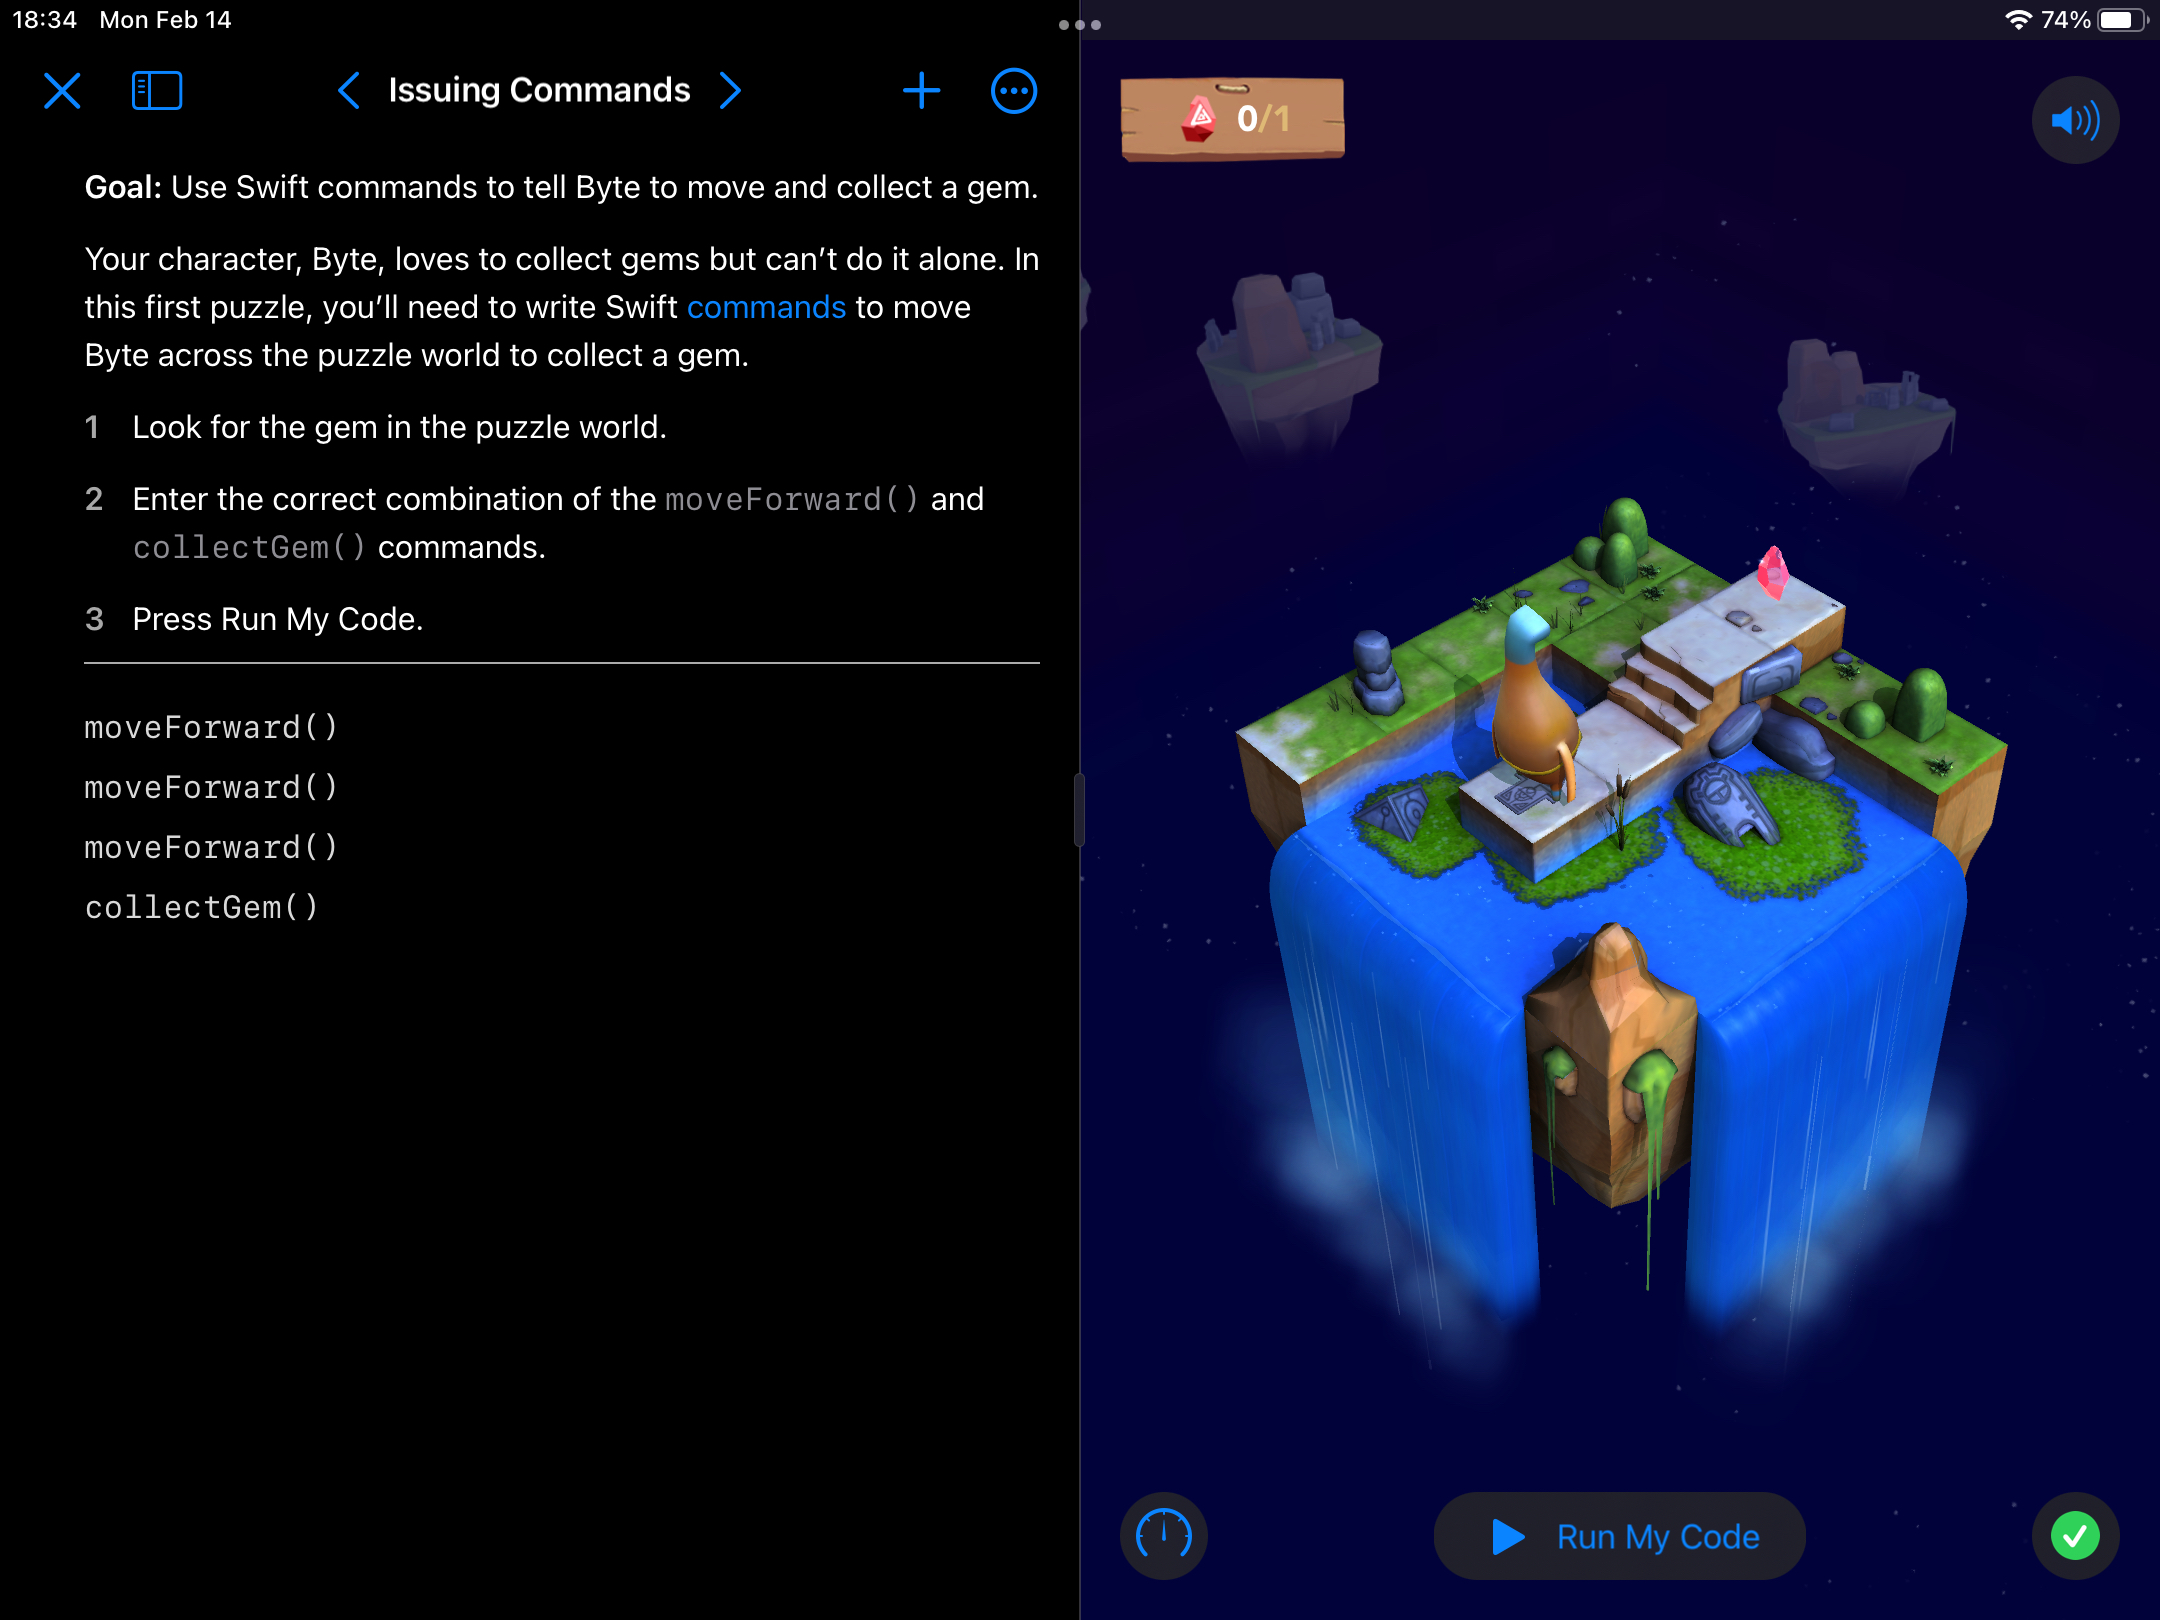
\includegraphics[width=1\textwidth]{images/Swift_Playground_iPad.jpeg}
\centering
\caption{\textit{Приказ апликације Swift Playgrounds на iPad-у}}
\label{slika:swift_playground_ipad}
\end{figure}

\begin{figure}[H]
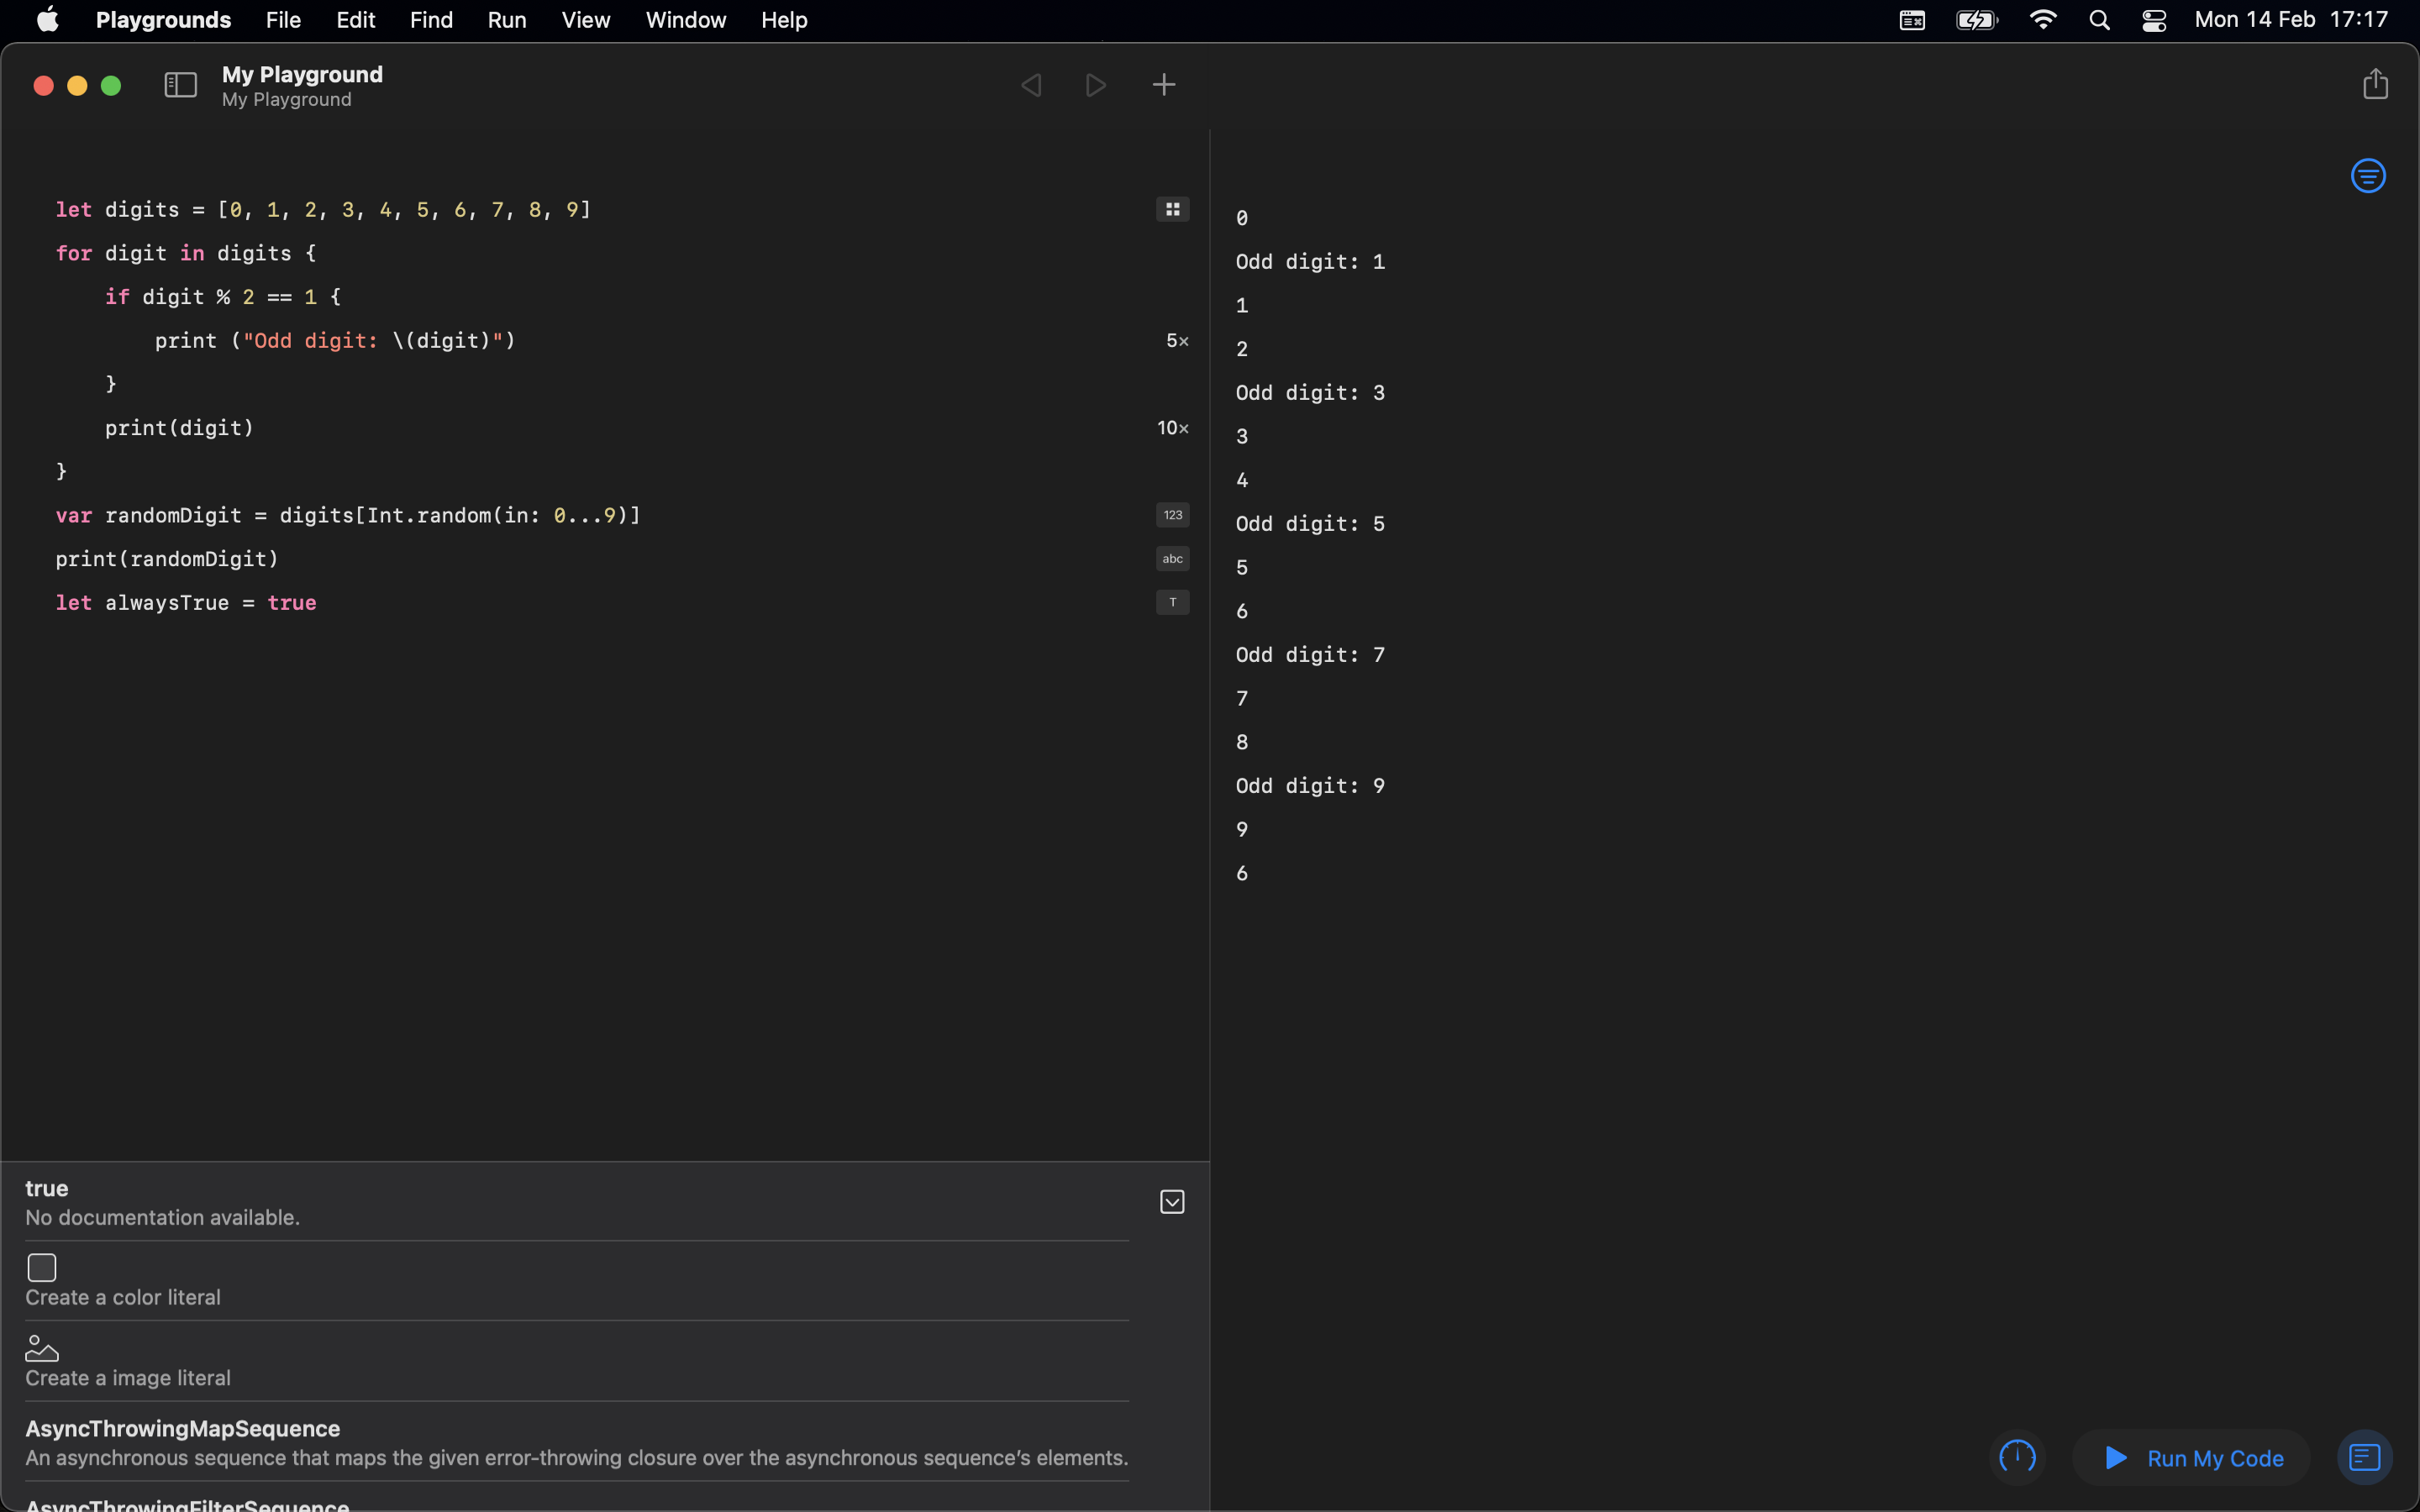
\includegraphics[width=1\textwidth]{images/Swift_Playground_macOS.png}
\centering
\caption{\textit{Приказ апликације Swift Playgrounds на macOS-у}}
\label{slika:swift_playground_macos}
\end{figure}

\subsection{Менаџер пакета}

\indent \textit{Swift} менаџер пакета (енг. \textit{Swift package manager}) је више-платформски алат за израду, покретање, тестирање и груписање \textit{Swift} библиотека и извршних датотека. Помоћу менаџера пакета могу се најлакше поделити библиотеке и изворни кодови. Конфигурација самог менаџера као и сам \textit{Swift} менаџер пакета су такође писани у \textit{Swift}-у, чинећи конфигурацију циљаних извршних датотека и управљање зависностима међу пакетима веома једноставним.

\section{Окружење за израду апликација са графичким интерфејсом \textit{SwiftUI}}
\label{sec:SwiftUI}

\indent \textit{SwiftUI} је радно окружење које служи за израду апликација са графичким интерфејсом погодним за све платформе компаније \textit{Apple}, користећи концизну моћ програмског језика \textit{Swift}. Омогућава креирање разноврсних апликација уз само један скуп алата и програмског интерфејса апликације (енг. \textit{application programming interface, API}) \cite{SwiftUI_Cookbook}.

\subsection{Основна структура}

\indent Радно окружење \textit{SwiftUI} пружа велики број погледа (енг. \textit{views}), контрола и распоредних структура (енг. \textit{layout structures}) који олакшавају процес израде корисничког интерфејса апликације. Уз то садржи и алате који управљају током података од модела до погледа и контрола\footnote{Архитектурни образац Модел-Поглед-Контролер (енг. \textit{Model-View-Controller}, MVC) који се заснива на подели на три целине, модел --- структура података, поглед --- приказ података у корисничком окружењу, контролор --- управљање моделом.}, са којима корисник може интераговати. Интеракција се одвија преко додира, гестова и других типова улазних података у апликацији који се потом обрађују помоћу обрађивача догађаја (енг. \textit{event handlers}).
\\
\indent Структура апликације се дефинише помоћу протокола \textit{App} и попуњава се сценама које садрже погледе чији скуп чини кориснички интерфејс апликације. \textit{SwiftUI} омогућава и креирање нових погледа, једини услов је да тај поглед имплементира протокол \textit{View}. Нови поглед се може комбиновати са другим, корисничким или погледима радног окружења, као што су текстуална поља, слике и многи други да би се направили комплекснији погледи који ће бити погодни за све кориснике апликације.

\subsection{Карактеристике}

\indent \textit{SwiftUI} је настао као наследник радног окружења \textit{UIKit}, а основна карактеристика која издваја радно окружење \textit{SwiftUI} од \textit{UIKit}-а је другачија програмска парадигма, конкретно декларативна синтакса. Више о разликама ова два радна окружења биће описано у поглављу \ref{subsec:Разлика SwiftUI и UIKit} --- \nameref{subsec:Разлика SwiftUI и UIKit}. 
\\
\indent Декларативна синтакса омогућава програмерима да једноставно опишу понашање корисничког интерфејса. К\^{o}д је много једноставнији за читање и разумевање као и за писање, чиме је обезбеђена значајна уштеда времена приликом писања новог кода и одржавања већ постојећег. Пример кода у \textit{SwiftUI}-у приказан је у делу \ref{lst:Пример SwiftUI кода} --- \nameref{lst:Пример SwiftUI кода}. Модификатор \textit{@State} биће објашњен у делу \ref{subsec:Стање и ток података} --- \nameref{subsec:Стање и ток података}.

\begin{lstlisting}[caption=\textit{{Пример SwiftUI кода}}, label={lst:Пример SwiftUI кода}, language=Swift, frame=single]
// Ucitavanje SwiftUI radnog okruzenja
import SwiftUI

// Kreiranje strukture koja ce sadrzati glavni pogled
struct Content : View {

    // Definisanje promenljive 'recepti'
    @State var recepti = RecepModel.listaRecepata
    
    // Definisanje tela pogleda
    var body: some View {
        // Izlistavanje svih recepata kroz listu
        List(recepti.stavke, action: recepti.izabranaStavka) { recept in
            // Prikaz slike
            Image(recept.slika)
            // Definisanje vertikalnog skupa elemenata
            VStack(alignment: .leading) {
                // Prikaz teksta
                Text(recept.ime)
                // Prikaz teksta sive boje
                Text(recept.vremePripreme)
                    .color(.gray)
            }
        }
    } 
}
\end{lstlisting}

\subsection{Стање и ток података}
\label{subsec:Стање и ток података}

\indent Декларативно програмирање омогућава да се за погледе вежу одговарајући модели података. Када год се неки од података промени, \textit{SwiftUI} аутоматски поново учита све погледе за који су промењени подаци везани и прикаже их кориснику, тако да програмер не мора бринути о томе. Ово се постиже променљивим стањима и везивањем, чиме се подаци везују за конкретне погледе. Тиме се остварује једини извор истине\footnote{Једини извор истине је начин структуирања информационих модела и шеме података тако да се сваки податак обрађује и мења на само једном месту.} (енг. \textit{single source of truth, SSoT}) за све податке и олакшава одржавање тачности података у сваком тренутку. 
\\
\indent У зависности од конкретне потребе у тренутној ситуацији, постоји више начина за остваривањем јединог извора истине:

\begin{itemize}
    \item \textit{State} --- Омогућава локално управљање стањем корисничког интерфејса, пример \ref{lst:Омотачи података --- State} --- \nameref{lst:Омотачи података --- State}. Када је променљива означена као \textit{State}, другом погледу се мора проследити са префиксом '\$' уколико се жели омогућити промена њене вредности.
    \item \textit{BindableObject} --- Користећи омотач својства \textit{ObservedObject}  може се приступити спољашњој референци на модел података који имплементира протокол \textit{ObservableObject}. Уколико је променљива смештена у спољашње окружење, може јој се приступити користећи омотач својства \textit{EnvironmentObject}. Инстанцирање посматрајућег (енг. \textit{observable}) објекта директно у погледу постиже се коришћењем модификатора \textit{State\-Object}.
    \item \textit{Binding} --- Користи се за дељење референце на једини извор истине, пример \ref{lst:Омотачи података --- Binding} --- \nameref{lst:Омотачи података --- Binding}.
    \item \textit{Environment} --- Подаци сачувани у \textit{Environment-у} се могу делити кроз целу апликацију, пример \ref{lst:Омотачи података --- Environment} --- \nameref{lst:Омотачи података --- Environment}.
    \item \textit{PreferenceKey} --- Прослеђивање података уз хијерархију погледа, од детета ка родитељу.
    \item \textit{FetchRequest} --- Управљање трајним подацима који се чувају унутар \textit{Core Data}.
\end{itemize}

Графички приказ модификатора може се видети на слици \ref{slika:data_flow_primitives} --- \nameref{slika:data_flow_primitives}.

\begin{figure}[H]
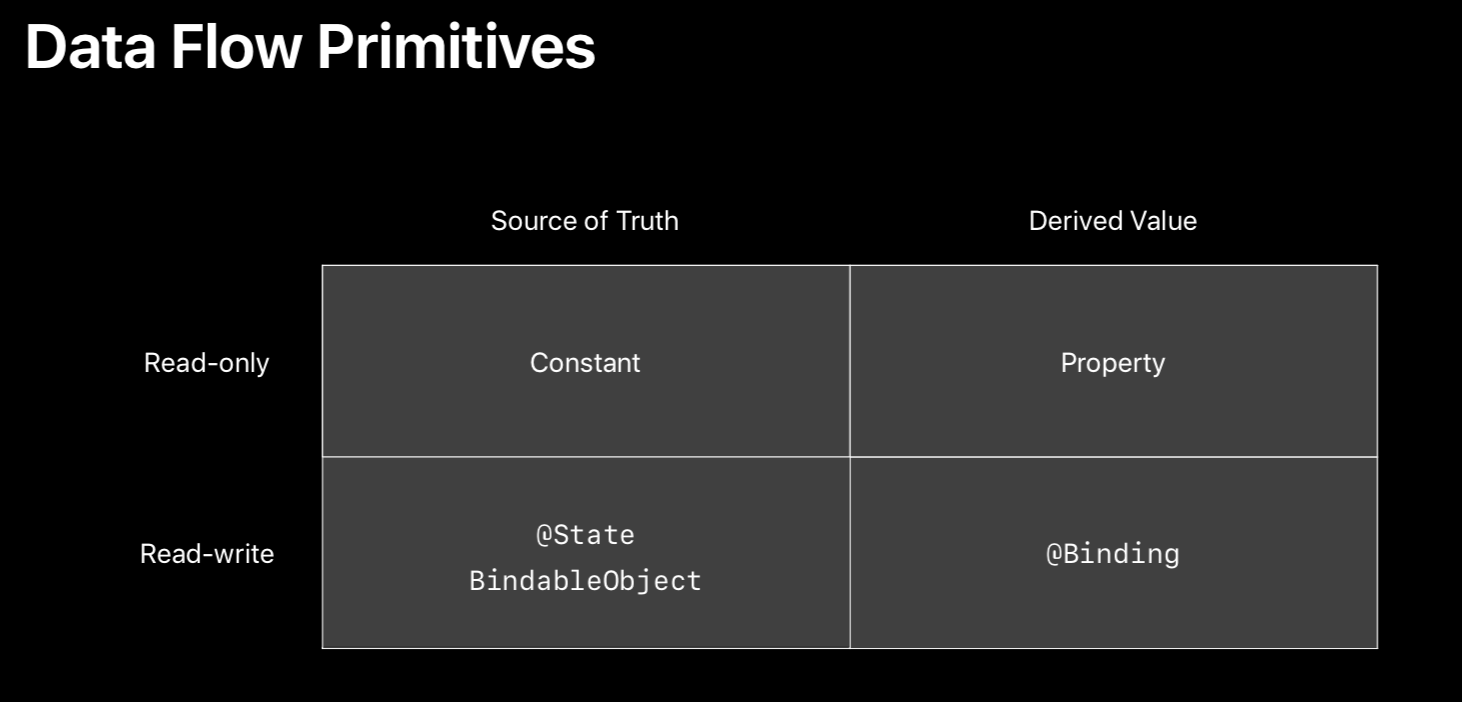
\includegraphics[width=1\textwidth]{images/DataFlowPrimitives.png}
\centering
\caption{\textit{Различити омотачи података}}
\label{slika:data_flow_primitives}
\end{figure}

\begin{lstlisting}[caption=\textit{{Омотачи података --- State}}, label={lst:Омотачи података --- State}, language=Swift, frame=single]
    struct Recept: View {
        var recept: ReceptPodatak
        @State private var daLiJeOmiljen = false
        
        var body: some View {
            VStack {
                Text(recept.ime)
                // 'OmiljenRecept' je pogled koji sadrzi zvezdicu koja oznacava da li je recept medju omiljenima (puna zvezdica --- jeste, prazna --- nije)
                OmiljenRecept(daLiJe: $daLiJeOmiljen)
            }
        }
    }
\end{lstlisting}

\begin{lstlisting}[caption=\textit{{Омотачи података --- Binding}}, label={lst:Омотачи података --- Binding}, language=Swift, frame=single]
    struct Recept: View {
    var recept: ReceptPodatak
    // Promenljiva 'daLiJeOmiljen' je definisana u jednom pogledu, a moze se menjati u drugom
    @Binding var daLiJeOmiljen: Bool

    var body: some View {
        Button(action: {
            // Akcija dugmeta koja menja promenljivu 'daLiJeOmiljen'
            self.daLiJeOmiljen.toggle()
        }) {
            // Provera promenljive 'daLiJeOmiljen' i prikaz odgovarajuce slike
            Image(systemName: daLiJeOmiljen ? "star.fill" : "star.empty")
        }
    }
}
\end{lstlisting}

\begin{lstlisting}[caption=\textit{{Омотачи података --- Environment}}, label={lst:Омотачи података --- Environment}, language=Swift, frame=single]
    struct Kulinarstvo_widgetEntryView : View {
    var entry: Provider.Entry
    
    // Cita podatke za 'widgetFamily' iz okruzenja aplikacije i smesta ih u promenljivu 'widgetFamily'
    @Environment(\.widgetFamily) var widgetFamily
    
    @ViewBuilder
    var body: some View {
        // U zavisnosti od promenljive 'widgetFamily' prikazuje se odgovarajuci widget
        switch widgetFamily {
        case .systemSmall:
            RecipeView(recipe: entry.recipe)
                .widgetURL(entry.recipe.url)
        case .systemMedium:
            RecipeMediumView(recipe: entry.recipe, ingredients: entry.recipe.ingredients.count > 3 ? Array(entry.recipe.ingredients.dropLast(entry.recipe.ingredients.count - 3)) : entry.recipe.ingredients)
        default:
            Text("")
        }
    }
}
\end{lstlisting}

\subsection{Разлика између радних окружења \textit{SwiftUI} и \textit{UIKit}}
\label{subsec:Разлика SwiftUI и UIKit}

\indent \textit{UIKit} и \textit{SwiftUI} су радна окружења развијена од стране \textit{Apple}-а, која помажу приликом израде корисничког интерфејса апликације. Генерално, највећа разлика између ова два радна окружења је у начину размишљања, како доћи до решења и како то решење касније имплементирати. Ова разлика ће бити показана на једном конкретном примеру. Креирање форме за пријављивање на одређени сајт уз креирање вертикалног скупа елемената, који ће бити хоризонтално и вертикално центрирани у скупу, а скуп ће се састојати од два текстуална поља (корисничко име и лозинка) и једног дугмета (са акцијом провере података).
\\
\indent Са \textit{UIKit}-ом мора се водити рачуна о свим ситним детаљима као што су: креирање вертикалног скупа елемената, његово додавање у главни поглед, креирање текстуалног поља, додавање текстуалног поља у скуп елемената, додавање аутоматског ограничења распореда како би се центрирало текстуално поље, понављање поступка за друго текстуално поље и поновно понављање поступка за дугме. 
\\
\indent За разлику од \textit{UIKit}-а, \textit{SwiftUI} се базира на декларативном начину програмирања и коришћењем радног окружења \textit{SwiftUI} је довољно навести груписање два текстуална поља и дугмета у вертиклани скуп елемената и у ком погледу ће се приказати. Све ситне детаље ће радно окружење одрадити само, онако како је то уобичајено (енг. \textit{default}) дефинисано. Наравно, програмер по потреби може и сам променити ове детаље.
\\
\indent Креирање корисничког интерфејса у \textit{UIKit}-у коришћењем само \textit{Swift} кода је веома компликовано, и за веће пројекте готово немогуће. Најчешћи начин израде корисничког интерфејса је коришћењем \textit{Storyboards-а} i \textit{Interface Builder-а}, помоћу којих програмер креира кориснички интерфејс превлачењем, спуштањем и конфигурацијом графичких елемената. У \textit{SwiftUI}-у се кориснички интерфејс изграђује помоћу \textit{Swift} кода. Корисник декларише шта ће бити креирано и радно окружење то уради. Да би процес креирања био бржи и приступачнији, од верзије \textit{Xcode}-а 11, која је изашла у исто време када је представљен \textit{SwiftUI}, постоји могућност прегледа уживо сваког појединачног погледа који је креиран или скупа више погледа одједном. О овоме ће бити више речи у поглављу \ref{subsec:Xcode - преглед уживо} --- \nameref{subsec:Xcode - преглед уживо}.
\\
\indent Уколико се сагледају архитектуре образаца, може се приметити да се \textit{UIKit} првенствено базира на \textit{MVC} обрасцу, док \textit{SwiftUI} користи \textit{MVVM}\footnote{Архитектурни образац Модел-Поглед-Модел погледа (енг. \textit{Model-View-ViewModel}) који се заснива на подели на три целине, модел --- структура података, поглед --- приказ података у корисничком окружењу, модел погледа --- стање података у моделу.} образац. За заинтересоване читаоце, постоји могућност комбиновања ова два радна окружења и коришћење \textit{SwiftUI}-а унутар \textit{UIKit} кода, или обратно.

\subsection{Преглед уживо --- Xcode}
\label{subsec:Xcode - преглед уживо}

\indent Са представљањем \textit{SwiftUI}-a, \textit{Apple} је представио и нову верзију њиховог ИРО-а \textit{Xcode11}, у коме је додато својство рада у новом радном окружењу као и могућност прегледа уживо сваког погледа. Предност оваквог начина писања кода је у могућности брзог визуелног прегледа измена без потребе поновне изградње (енг. \textit{rebuilding}) апликације. Ова предност највише долази до изражаја када се ради на додавању или измени погледа који се налази дубоко унутар навигације апликације и за који је потребно више кликова и/или превлачења (приликом тестирања измена кода) да би се до њега дошло. 
\\
\indent Преглед уживо помаже да се у \textit{SwiftUI}-у користи метод превлачења и пуштања (енг. \textit{drag and drop}) за креирање корисничког интерфејса, тако што се сваки елемент превлачи у део где се пише к\^{o}д и када се испусти, тај елемент постаје део кода. Избор графичких елемената може се видети на слици \ref{slika:d&d1}, док је к\^{o}д програма и приказ уживо након испуштања графичког елемента \textit{Text} приказан на слици \ref{slika:d&d2}.

\begin{figure}[H]
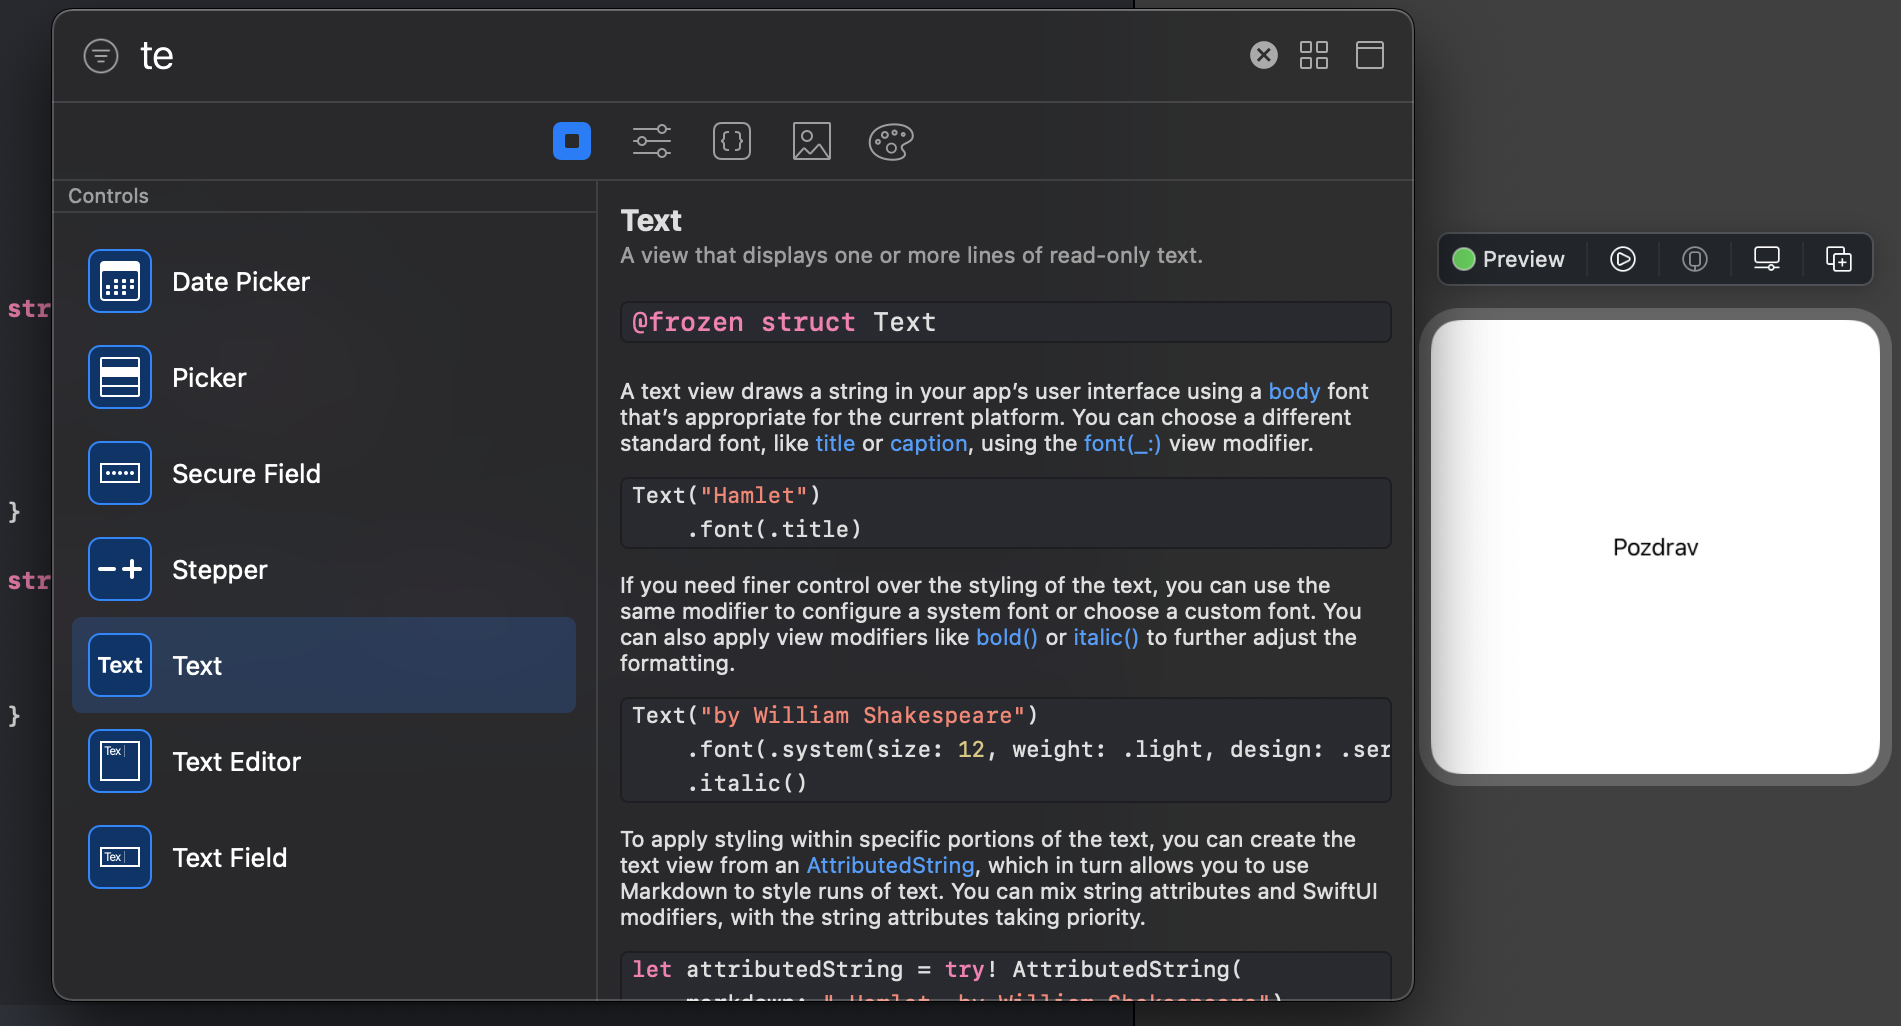
\includegraphics[width=1\textwidth]{images/Drag_and_drop_1.png}
\centering
\caption{\textit{Приказ графичких елемената}}
\label{slika:d&d1}
\end{figure}

\begin{figure}[H]
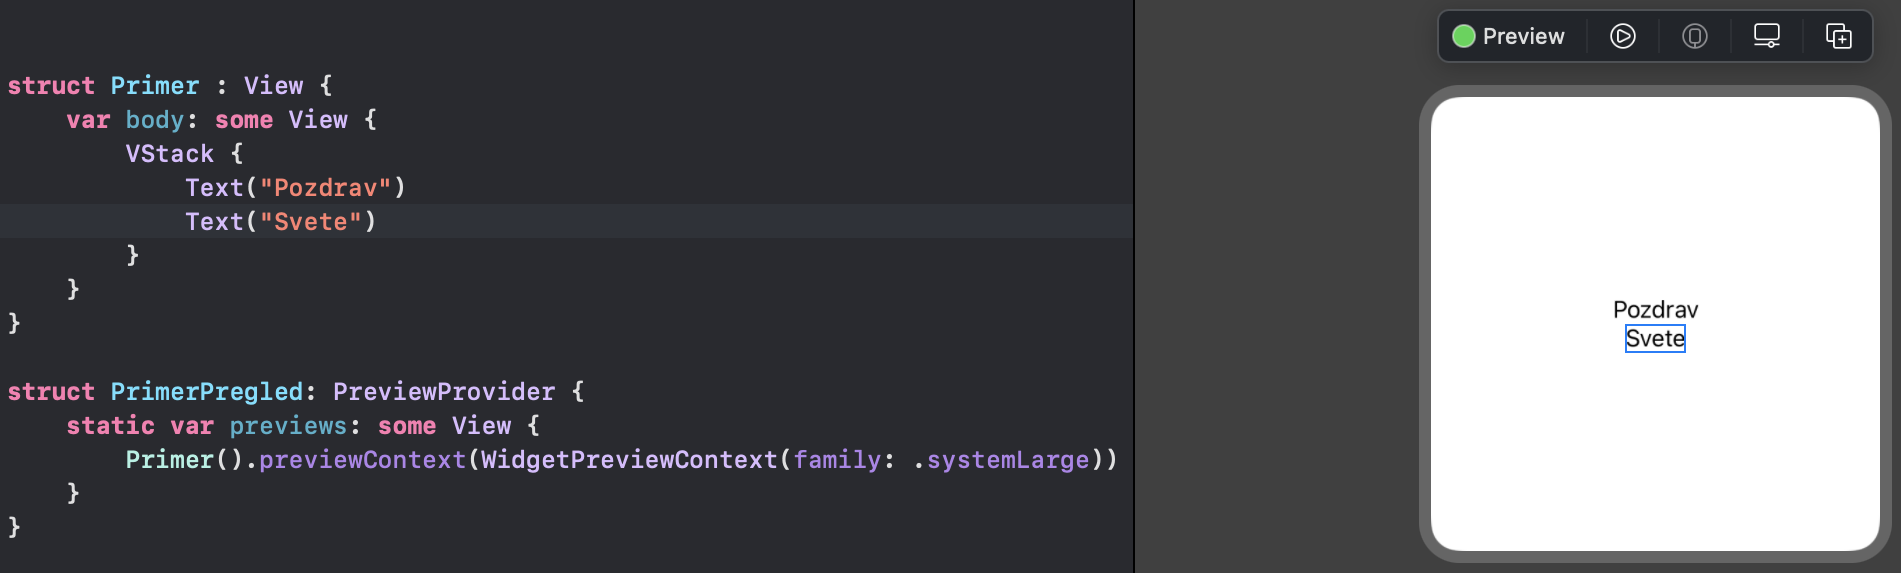
\includegraphics[width=1\textwidth]{images/Drag_and_drop_2.png}
\centering
\caption{\textit{К\^{o}д програма након испуштања елемента}}
\label{slika:d&d2}
\end{figure}

Да би се омогућило коришћење приказа уживо, инстанца жељеног погледа се смешта унутар тела структуре која имплементира протокол \textit{PreviewProvider}, а која служи за живи приказ погледа или групе погледа. Пример употребе структуре која имплементира протокол \textit{PreviewProvider} може се видети у делу \ref{lst:Xcode - преглед уживо} --- \nameref{lst:Xcode - преглед уживо}.

\begin{lstlisting}[caption=\textit{{Xcode --- преглед уживо}}, label={lst:Xcode - преглед уживо}, language=Swift, frame=single]
    
    struct PlaceholderView : View {
        var body : some View {
            Kulinarstvo_widgetEntryView(entry: SimpleEntry(date: Date(), configuration: ConfigurationIntent(), recipe: RecipeModel.testData[0]))
        }
    }
    
    // Struktura u kojoj se konfigurise prikaz uzivo
    struct Kulinarstvo_widget_Previews: PreviewProvider {
        static var previews: some View {
            // Grupisanje vise pogleda
            Group {
                // Prikaz malog widget-a sa prvim elementom iz liste
                Kulinarstvo_widgetEntryView(entry: SimpleEntry(date: Date(), configuration: ConfigurationIntent(), recipe: RecipeModel.testData[0]))
                    .previewContext(WidgetPreviewContext(family: .systemSmall))
                
                // Prikaz srednjeg widget-a sa skrivenim sadrzajem
                PlaceholderView()
                    .previewContext(WidgetPreviewContext(family: .systemMedium))
                    .redacted(reason: .placeholder)
            }
        }
    }    
\end{lstlisting}

\indent Након сваке измене која се направи у коду који је везан за поглед(е) који се налази у прегледу уживо, \textit{Xcode} ће изнова направити нову верзију и покренути је у прозору за преглед уживо. Преглед уживо не мора приказивати само један поглед, већ се могу груписати различити погледи и сви бити приказани одједном. Предност оваквог приступа је могућност истовременог прегледа старог и новог изгледа погледа, више величина виџета, истих погледа са светлом и тамном бојом позадине, погледа на различитим језицима...

\indent Више на тему прегледа погледа уживо може се наћи у оквиру предавања \href{https://developer.apple.com/videos/play/wwdc2019/233/}{\textit{Mastering Xcode Previews}} \cite{Mastering_Xcode_Previews} и \href{https://developer.apple.com/videos/play/wwdc2020/10149/}{\textit{Structure your app for SwiftUI previews}} \cite{Structure_your_app_for_SwiftUI_previews} са \textit{Apple}-ове конференције за програмере из 2019. и 2020. године респективно.

\chapter{Улога и развој виџетa}

\indent Виџет на уређајима са платформом компаније \textit{Apple} приказује крајњим корисницима изабрани кључни део апликације. Виџет је за сада једини део апликације који у потпуности мора бити развијен коришћењем окружења \textit{SwiftUI}.

\section{Основне карактеристике виџета}

\indent Виџет се приказује крајњим корисницима тамо где ће се најлакше уочити, на \textit{iPhone}-у и \textit{iPad}-у се може налазити на почетном екрану или у делу \textit{Today View}-а, док се на \textit{Mac} уређајима налази у центру за нотификације. Величина виџета није флексибилна као на \textit{Android} уређајима, па тако постоји могућност креирања малих, средњих и великих, а од верзије оперативног система \textit{iPadOS15} екстра великих (само за \textit{iPad} уређаје) виџета. Величина малог виџета је $2 \times 2$ места на почетном екрану \textit{iPhone}-а, величина средњег је $2 \times 4$, велики виџет заузима $4 \times 4$ места на екрану, док је величина екстра великих виџета $4 \times 8$.
\\
\indent Скуп свих тренутно доступних виџета на уређају налази се у галерији виџета (енг. \textit{widget gallery}), која помаже корисницима приликом одабира конкретне величине и типа виџета (једна апликација може имати више типова виџета). Режим за измену виџета унутар галерије омогућава корисницима да контролишу и мењају своје виџете и тиме их прилагоде себи. Измена виџета ће бити доступна корисницима уколико је она омогућена од стране програмера приликом креирања виџета. Више речи о овоме биће у делу \ref{sec:Развој виџетa} --- \nameref{sec:Развој виџетa}.
\\
\indent На оперативним системима \textit{iOS} и \textit{iPadOS} галерија има могућност додавања паметних гомила (енг. \textit{smart stack}), које могу садржати до десет различитих виџета исте величине. Паметна гомила у једном тренутку приказује један од виџета који се налазе у њој. Корисник може сам да мења који ће виџет бити приказан једноставним померањем (енг. \textit{scrolling}). Временом, паметна гомила може научити који виџет корисник ставља на почетак гомиле у току дана (или недеље) и сама мењати примарне виџете у одређеном тренутку (на пример, након гашења аларма прво се приказује виџет са временском прогнозом, па најновије вести, стање у саобраћају).
\\
\indent \textit{Siri} асистент\footnote{Интелигентни лични асистент на уређајима са платформом компаније \textit{Apple}.} може и сам додати виџете у паметну гомилу уколико претпостави да постоји неки виџет који би кориснику био користан. Након тога корисник сам одлучује да ли жели да новододати виџет остане у паметној гомили или не.

\subsection{Радно окружење \textit{WidgetKit}}
\indent \textit{WidgetKit} је радно окружење које уз \textit{widget API} из  \textit{SwiftUI}-а служи за израду виџета, од његовог изгледа, преко временског ажурирања па све до омогућавања конфигурације виџета од стране крајњих корисника и управљања паметном гомилом приликом ротације виџета од стране система. Још једна могућност коју ово радно окружење пружа је повезивање апликације и самог виџета, што омогућава кориснику да отвори апликацију притиском на виџет и аутоматски оде на одговарајући поглед из виџета када жели да види детаљније податке. Програмери морају обратити пажњу код оваквог начина комуникације, виџет не би смео да служи само као пречица за покретање апликације јер то може довести до престанка употребе виџета од стране корисника. Лакше је додати саму апликацију на почетни екран која истовремено заузима мање простора него виџет (више о томе биће објашњено у делу \ref{sec:Дизајн виџетa} --- \nameref{sec:Дизајн виџетa}).

\section{Развој виџетa}
\label{sec:Развој виџетa}
\indent Виџет је \textit{SwiftUI} поглед. Виџети су тренутно једини део апликација развијених за платформе компаније \textit{Apple} који у потпуности морају бити написани коришћењем радног окружења \textit{SwiftUI}. \textit{Apple} је од почетка развоја виџета имао на уму овакву идеју због начина њиховог приказивања, повременог ажурирања података, као и немогућности корисничке интеракције са самим виџетима (осим једноставног клика којим се отвара одређени део апликације).

\subsection{Додавање виџет додатка апликацији}
\indent Додатак апликације (енг. \textit{app extension}) је проширење апликације\footnote{Обично се састоји од пар фајлова које ИРО аутоматски генерише и групише у посебан фолдер. Унутар фајлова је имплементиран одговарајући шаблон, који корисник допуњује или мења како би додатак одговарао апликацији.} које пружа додатне функционалности и садржај апликације крајњим корисницима у тренуцима када је не користе. Неки од додатака апликације су: додатак паметног сата (енг. \textit{watch extension}) који омогућава креирање додатка апликације намењеног паметним сатовима компаније \textit{Apple}, додатак центра за обавештења (енг. \textit{notification center extension}) који омогућава прилагођавање изгледа обавештења, виџет додатак (енг. \textit{widget extension}) који омогућава креирање виџета за конкретну апликацију.
\\
\indent Шаблон за виџет додатак креира основне компоненте потребне за његову израду. Унутар овог додатка корисник креира све потребне виџете за своју апликацију, независно од њиховог броја и величине. У одређеним ситуацијама различити типови виџета могу бити одвојени у посебним додацима. Ово се најчешће односи када један тип виџета захтева одређене дозволе од стране корисника, док за други тип оне нису потребне (на пример, приступ тренутној локацији корисника).

\indent Кораци за креирање виџет додатка:
\begin{enumerate}
    \item Отворити пројекат у \textit{Xcode}-у и изабрати \textit{File -> New -> Target}
    
    \item Из групе \textit{Application Extension}, изабрати \textit{Widget Extension} и кликнути \textit{Next}
    
    \item Унети име додатка и изабрати тим (који може чинити и једна особа) који ради на пројекту
    
    \item Уколико виџет подржава конфигурацију од стране корисника, штиклирати поље \textit{Include Configuration Intent}
    
    \item Кликнути на дугме \textit{Finish}
    
\end{enumerate}

\subsection{Додавање детаља конфигурације}
\indent Шаблон виџет додатка пружа иницијалну поставку програма виџет додатка који имплементира \textit{Widget} протокол. Два могућа начина конфигурације виџета су статичка (\textit{StaticConfiguration}) и конфигурација са сврхом (\textit{IntentConfiguration}). \\
\indent Статичка конфигурација се користи за виџете који немају параметре који могу бити конфигурисани од стране корисника. Пример виџета који нема конфигурабилне параметре је виџет системске апликације \textit{Screen time} који води статистику о активном времену проведеном на одговарајућем уређају. Конфигурација са сврхом се користи за виџете чији одређени параметри могу бити конфигурисани од стране корисника. Пример виџета са конфигурабилним параметрима је виџет системске апликације за временску прогнозу, где корисник може изабрати одређени град за који жели да добија податке. Ова конфигурација ће бити укључена, и конфигурациони фајл ће бити додат уколико програмер приликом додавања виџет додатка штиклира поље \textit{Include Configuration Intent}.
\\
\indent Да би програмер спровео почетну конфигурацију виџета потребно је да проследи следеће параметре:
\begin{description}
    \item [Тип] (енг. \textit{kind}), стринг који идентификује виџет, требао би да казује шта виџет представља.
    \item [Снабдевач] (енг. \textit{provider}), објекат класе која имплементира протокол \textit{Time\-lineProvider} и кроз временску линију коју производи одређује у ком тренутку ће виџет бити поново изрендерован и нови подаци бити приказани. Детаљније објашњење начина функционисања временске линије дато је у делу \ref{subsec:Временска линија} --- \nameref{subsec:Временска линија}.
    \item [Затворење садржаја] (енг. \textit{content closure}), затворење које садржи \textit{SwiftUI} поглед и које \textit{WidgetKit} позива када дође време за поновно рендеровање садржаја виџета.
    \item [Прилагођена сврха] (енг. \textit{custom intent}), фајл који дефинише параметре које корисник може мењати и прилагођавати себи. Израда овог фајла и његова конкретна употреба приликом израде виџета приказана је у делу \ref{subsec:Intent} --- \nameref{subsec:Intent}.
\end{description}

\indent Пример почетне статичке конфигурације виџета може се видети у коду \ref{lst:виџет - почетна конфигурација} --- \nameref{lst:виџет - почетна конфигурација}. Да би се подесила боја шеме прослеђује се променљива \textit{colorScheme} којом се боја виџета усклађује са системском бојом уређаја. Променљива \textit{kind} служи за јединствену идентификацију типа виџета. 

\begin{lstlisting}[caption=\textit{{Виџет --- почетна конфигурација}}, label={lst:виџет - почетна конфигурација}, language=Swift, frame=single]
    struct KulinarstvoRandomRecipesWidget: Widget {
        @Environment(\.colorScheme) var colorScheme
        
        let kind: String = "KulinarstvoSlasnoIEfikasnoRandomRecipesWidget"
        
        var body: some WidgetConfiguration {
            StaticConfiguration(kind: kind, provider: RandomRecipesProvider()) { entry in
                KulinarstvoRandomRecipesWidgetEntryView(entry: entry)
            }
            .configurationDisplayName("Recept na klik")
            .description("Dodaj svoje omiljene recepte na pocetni ekran")
            .supportedFamilies([.systemLarge])
        }
    }
\end{lstlisting}

\subsection{Временска линија}
\label{subsec:Временска линија}
\indent Снабдевач временске линије генерише временску линију која се састоји од уноса (енг. \textit{entries}), а сваки унос садржи датум и време када је потребно ажурирати садржај виџета. Када се датум и време из уноса подударе са реалним временом, \textit{WidgetKit} позива затворење садржаја које потом приказује ажуриране податке. 
\\
\indent Да би виџет био приказан у виџет галерији, \textit{WidgetKit} захтева од снабдевача преглед снимка (енг. \textit{preview snapshot}). Дохватање прегледа снимка се разрешава коришћењем променљиве \textit{isPreview} којом се проверава да ли снабдевач прегледа снимка шаље тренутни снимак за приказ у галерији или за приказ виџета на почетном екрану. Када је параметар \textit{isPreview} тачан, виџет се приказује у галерији. Уколико унутар виџета треба да буду приказани и одређени подаци који још увек нису учитани, постоје два решења. Могу се приказати подразумевани, унапред одређени подаци, или се могу користити подаци који чувају место правим подацима (енг. \textit{placeholder}). У примеру \ref{lst:виџет - placeholder} --- \nameref{lst:виџет - placeholder} може се видети креирање погледа чувара места (енг. \textit{placeholder view}) коришћењем статичких података који су увек доступни. Такође је приказана и имплементација чувара места у прегледу уживо са сакривеним подацима (енг. \textit{redacted data}) --- приказ како ће корисник видети виџет док не пристигну конкретни подаци у одређеним ситуацијама.

\begin{lstlisting}[caption=\textit{{Виџет --- placeholder}}, label={lst:виџет - placeholder}, language=Swift, frame=single]
    struct PlaceholderView : View {
        var body : some View {
            Kulinarstvo_widgetEntryView(
                entry: SimpleEntry(date: Date(), configuration: ConfigurationIntent(), recipe: Datafeed.shared.favRecipes[0], parameterToShow: MainParameter.Sastojci.rawValue))
        }
    }
    
    struct Kulinarstvo_widget_Previews: PreviewProvider {
        static var previews: some View {
             PlaceholderView()
                .previewContext(WidgetPreviewContext(family: .systemLarge))
                .redacted(reason: .placeholder)
        }
    }
\end{lstlisting}

\indent Када се подаци учитају, снабдевач добија обавештење, сакупља учитане податке и приказује виџет са њима. Након што корисник дода виџет на почетни екран и буде приказан иницијални снимак изгледа виџета, \textit{WidgetKit} позива функцију \textit{getTimeline} из провајдера, чиме захтева временску линију.

\subsection{Конфигурација са сврхом}
\label{subsec:Intent}
\indent Виџети представљају погледе који не интерагују са корисницима, односно не подржавају интерактивне елементе. Једина интеракција корисника са виџетом постиже се омогућавањем конфигурације виџета од стране корисника употребом фајла \textit{Intent}. У њему се наводе сви параметри које корисник може да промени (као и дозвољене вредности за те параметре). 
\\
\indent Да би се додали параметри које корисник може да конфигурише постоје предуслови који се морају испунити:
\begin{itemize}
    \item додавање дефиниције \textit{Intent}-а који дефинише конфигурабилне параметре,
    \item структура 'снабдевач временске линије' имплементира протокол \textit{IntentTi\-melineProvider} уместо протокола \textit{Timeli\-neProvider}, да би конфигурација параметара од стране корисника била сачувана у уносима временске линије,
    \item уколико параметри зависе од динамичких података потребно је имплементирати екстензију \textit{Intent}-а.
\end{itemize}

\indent На слици \ref{slika:widget_configuration} се може видети изглед конфигурације виџета који има два параметра, први служи за избор рецепта који ће у виџету бити приказан, а други за избор примарног параметра који ће бити приказан уз опис рецепта (састојци или припрема).

\begin{figure}[H]

\includegraphics[width=0.5\textwidth]{images/Widget_configuration.png}
\centering
\caption{\textit{Конфигурација виџета}}
\label{slika:widget_configuration}
\end{figure}

\subsection{Везе унутар виџета}
\indent Једини начин директне комуникације између корисника и виџета остварена је везама (енг. \textit{links}) унутар виџета. Када корисник кликне на виџет отвара се апликација којој тај виџет припада, а програмер може конфигурисати који део апликације ће бити приказан кориснику у зависности од елемента унутар виџета на који је кликнуо.
\\
\indent За све величине виџета, осим малих, може се користити веза (енг. \textit{link}) која се додаје једном погледу унутар виџета. Том везом је одређено тачно место у апликацији које ће бити отворено уколико корисник кликне на одговарајући поглед (на пример, виџет који садржи листу са три рецепата и сваки елемент листе има везу која води ка детаљној страни о том рецепту. Када корисник кликне на одговарајући рецепт отвориће се апликација и приказати страницу са детаљним описом рецепта на који је корисник кликнуо). Све величине виџета могу користити модификатор \textit{widgetURL(\_:)}. Овај модификатор ће бити активиран уколико корисник кликне на поглед унутар виџета који нема дефинисану везу и биће отворена апликација, уз могућу додатну навигацију уколико је дефинисана приликом додавања модификатора. У примеру кода \ref{lst:Везе унутар виџета} --- \nameref{lst:Везе унутар виџета} приказана је употреба модификатора \textit{widgetURL(\_:)} за мале виџете, као и употреба веза за средње и велике виџете.

\begin{lstlisting}[caption=\textit{{Везе унутар виџета}}, label={lst:Везе унутар виџета}, language=Swift, frame=single]
    struct Kulinarstvo_widgetEntryView : View {
        var entry: Provider.Entry
        @Environment(\.widgetFamily) var widgetFamily
        
        @ViewBuilder
        var body: some View {
            switch widgetFamily {
            case .systemSmall:
                ImageRecipeView(recipe: entry.recipe, isSmallView: true)
                    .widgetURL(entry.recipe.url)
            case .systemMedium:
                Link(destination: entry.recipe.url ?? URL(fileURLWithPath: "")) {
                    RecipeMediumView(recipe: entry.recipe, listName: entry.parameterToShow)
                }
            case .systemLarge:
                Link(destination: entry.recipe.url ?? URL(fileURLWithPath: "")) {
                    RecipeLargeView(recipe: entry.recipe, mainParameter: entry.parameterToShow)
                }
            default:
                Text("")
            }
        }
    }
\end{lstlisting}

\subsection{Више типова виџета у једном виџет додатку}
\indent Уколико постоји потреба за коришћењем више различитих типова виџета у једном виџет додатку, то се може постићи уз пар измена главне структуре виџет додатка (структура означена анотацијом \textit{@main}). Уместо протокола \textit{Widget}, главна структура виџет додатка мора имплементирати протокол \textit{WidgetBundle}. Тело структуре треба да имплементира протокол \textit{Widget} и да буде означен анотацијом \textit{@WidgetBundleBuilder}. Приказ употребе више типова виџета у једном виџет додатку може се видети у примеру \ref{lst:Више виџета у једном виџет додатку} --- \nameref{lst:Више виџета у једном виџет додатку}.

\begin{lstlisting}[caption=\textit{{Више виџета у једном виџет додатку}}, label={lst:Више виџета у једном виџет додатку}, language=Swift, frame=single]
    @main
    struct ReceptiWidgets: WidgetBundle {=
        @WidgetBundleBuilder
        var body: some Widget {
            DetaljanPrikazReceptaWidget()
            ListaRecepataWidget()
            SpisakZaKupovinuWidget()
        }
    }
\end{lstlisting}

\section{Дизајн виџетa}
\label{sec:Дизајн виџетa}

\indent Главна улога виџета је приказивање садржаја који кориснику пружа корисне информације без покретања апликације. Самим тим подаци морају бити тачни и релевантни за корисника, сам виџет би требао бити конфигурабилан како би кориснику допустио одређену врсту слободе приликом коришћења и дизајниран тако да одговара апликацији којој припада.

\subsection{Фокус виџетa}
\indent  Подаци које виџет приказује треба да буду минималистички, да одговарају величини виџета (већа величина треба да повлачи и већу количину података) и да буду временски и кориснички релевантни. Први корак у дизајну виџета је избор дела апликације који ће тај виџет представљaти. 
\\
\indent Свака величина виџета која је омогућена за додавање из галерије треба да садржи одређену количину информација која је пропорционална тој величини. Не сме се дозволити да неколико величина виџета приказују исте податке, али истовремено приликом додавања нових података се мора водити рачуна о почетној идеји, односно делу апликације које тај виџет треба да представља. Уколико не постоји довољна количина података за веће виџете, те величине виџета могу бити искључене из понуде кориснику.
\\
\indent Виџет не би смео да служи само као пречица за покретање апликације. Корисници очекују од сваког виџета да им покаже корисне информације, у супротном неће наићи на добар одзив и истовремено може бити штетно самој апликацији (мањи број корисника, лошија оцена у продавници).

\subsection{Ажурни подаци}
\indent Да би виџети могли да пружају корисне и прецизне информације подаци које приказују морају бити ажурирани. Виџети не подржавају ажурирање података у реалном времену, а и сам оперативни     систем може ограничити ажурирање података које виџет приказује у завиности од корисничког понашања и интеракције са њим, па се мора пронаћи начин на који ће подаци у виџету увек бити релевантни. 
\\
\indent Потребно је пронаћи оптимално време за ажурирање података у виџету, узимајући у обзир колико се сами подаци које виџет приказује често мењају. Једна корисна информација која се може приказати уз временски зависне податке је поље које ће представљати датум и време када су подаци последњи пут ажурирани. За одређене податке се може искористити помоћ система за одређивање датума и времена (на пример, виџет који приказује време у које ће се огласити аларм, истовремено може приказивати и ажуран податак о томе колико је времена остало до оглашавања аларма).

\subsection{Конфигурабилност и интеракција}
\indent У већини случајева виџет треба да омогући кориснику конфигурабилност како би могао да пружи релевантне информације (на пример, књига коју корисник тренутно чита у апликацији \textit{Apple Books}), док поједини виџети не морају бити конфигурабилни (на пример, најновије вести). Уколико је виџет конфигурабилан, потребно је да подешавања буду једноставна и да се не захтева превише информација од корисника. Кориснички интерфејс за измену виџета је унапред одређен и исти за све виџете, као што је показано у делу \ref{subsec:Intent} --- \nameref{subsec:Intent}.

\subsection{Дизајн прилагођен свима}
\indent Виџети треба да буду јарких боја како би се истицали на екрану, али треба да садрже јасно видљив текст како би корисник могао да види све потребне информације након откључавања или непосредно пре закључавања уређаја. Виџет треба прилагодити апликацији коју представља (боје, фонт текста, јединствени елементи...), док истовремено не треба истицати превише елемената који ће указивати на апликацију (лого, име) јер се тиме само непотребно заузима простор унутар виџета који се може боље искористити.  
\\
\indent Количина информација која ће бити приказана у виџету мора бити оптимална. Уколико се прикаже премало информација виџет неће имати превелики значај за кориснике, док превише информација на малом простору отежава читање и разумевање података.
\\
\indent Израда дизајна виџета за обе врсте боја системске позадине (светле и тамне) је веома важно како би виџет био прихваћен од стране свих корисника. Дизајн виџета се не сме разликовати од системске боје позадине јер ниједан корисник не жели видети таман текст на светлој боји позадине уколико је изабрао тамну системску боју позадине. Приликом израде обе врсте дизајна може помоћи \textit{Xcode preview} који омогућава истовремено сагледавање оба дизајна, упоређивање и исправљање евентуалних недостатака.
\\
\indent \textit{Apple} саветује да се никад не користи фонт текста мањи од 11 поена\footnote{\textit{Apple}-ов израз за "број који треба уписати у поље", универзална мера у дизајну на платформама компаније \textit{Apple}.}. Коришћење мањег фонта би корисницима знатно отежало употребу виџета. Увек треба користити званичне погледе (погледи дефинисани унутар радног окружења \textit{SwiftUI}) за приказ текста, како би се омогућила скалабилност текста, као и системско читање текста (читање текста употребом виртуелног асистента).
\\
\indent Пажњу треба обратити на дизајн прегледа виџета унутар галерије, за све типове и величине који виџет подржава, као и приказ чувара места уместо реалних података уколико они нису пристигли на време са сервера и не постоје подразумевани подаци. Уколико се исти елементи налазе у апликацији и истовремено на виџету потребно је да имају исту функционалност јер би у супротном корисници били збуњени. 
\\
\indent Потребно је искористити могућност приказа описа виџета у галерији и саставити кратак и јасан опис функционалности виџета. Груписање свих величина једног типа виџета са јединственим описом је погодно корисницима апликације, пре свега због једноставности разумевања коришћења виџета.

\chapter{Имплементација и визуелни приказ апликације}

\indent У овом поглављу биће представљена апликација "Кулинарство --- сласно и ефикасно" која прати мастер рад. Апликација треба да помогне корисницима приликом избора и припреме оброка, док виџет који је имплементиран у склопу апликације може послужити као подсетник за потребне састојке или кораке припреме и истовремено бити употребљен за предлагање наредних оброка. Изворни к\^{o}д апликације може се наћи на \textit{GitHub}-у \cite{Kulinarstvo_slasno_i_efikasno}.

\section{Карактеристике имплементације}

\indent Апликација "Кулинарство --- сласно и ефикасно" је развијена у ИРО-у \textit{Xcode}, коришћењем програмског језика \textit{Swift 5.5}. Виџет додатак је креиран употребом радног окружења \textit{SwiftUI}.

\subsection{Имплементација архитектуре \textit{MVC}}

Као архитектурални образац коришћена је архитектура \textit{MVC}, чиме је структура изворног кода подељена у три целине (модел, поглед и контролер). Унутар модела су дефинисане три класе, \textit{Ingredient} којом су описани састојци рецепта, \textit{Recipe} унутар које су дефинисана поља једног рецепта и \textit{RecipeModel} у којој су дефинисане методе које учитавају и парсирају податке о тренутно доступним рецептима из \textit{JSON}\footnote{\textit{JSON} (\textit{JavaScript Object Notation}) је текстуални формат дизајниран за размену података који је људима лак за читање и писање, а у програмском коду једноставан за генерисање и парсирање.} фајла ("\textit{RecipesData.json}"). Када се апликација први пут инсталира, биће учитан подразумевани фајл који долази уз апликацију, док ће сваки наредни пут бити учитан локални фајл који ће садржати све промене које је корисник унео (нове рецепте, омиљене рецепте). Дефиниција ових класа је приказана на слици \ref{slika:класе_модела}. Преостале класе које сачињавају модел су \textit{Datafeed} која служи за чување низа рецепата у завиности да ли припадају општем делу, омиљеним рецептима или рецептима које је корисник креирао, и \textit{AppTheme} у којој су дефинисане основне боје апликације за светлу и тамну боју системске позадине.

\begin{figure} [H]
    \centering
    \captionsetup{justification=centering}
    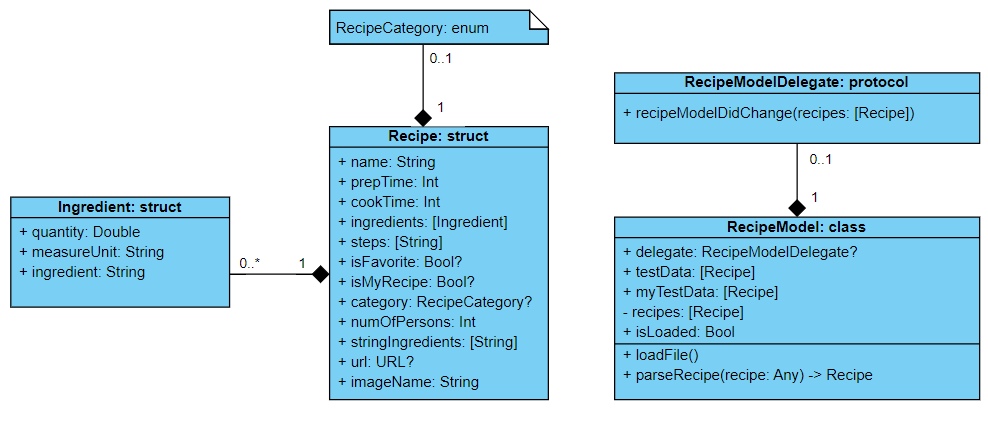
\includegraphics[width=1\textwidth]{images/class_diagram.png} 
    \caption{\textit{Дијаграм класа модела}}
    \label{slika:класе_модела}
\end{figure}

\subsection{Опис главних и помоћних погледа}

Компонента поглед дефинише главне и помоћне погледе који се користе у апликацији. Изглед главних погледа као и њихова повезаност може се видети на слици \ref{slika:главни_погледи}. Приликом почетног учитавања апликације приказује се улазни поглед (енг. \textit{entry view}), који је у овом случају празан поглед. Након њега се учитава и приказује главни поглед (\textit{TabBarViewController}) који се састоји из три дела (енг. \textit{tab}). Део са прегледом свих рецепата који се приказује на почетку, део који садржи омиљене рецепте корисника и део са рецептима које је тренутни корисник додао. Уколико корисник кликне на неки од рецепата (у било ком делу) биће му приказан детаљан опис рецепта (конкретан пример приказа погледа детаљног рецепта може се видети у делу \nameref{subsec:детаљан_рецепт} --- \ref{subsec:детаљан_рецепт}). У случају одабира додавања новог рецепта у делу "Моји рецепти" приказаће се поглед \textit{AddNewRecipeViewController} из којег је могуће отворити поглед који приказује додавање састојака и корака припреме рецепта.

\begin{figure} [H]
    \centering
    \captionsetup{justification=centering}
    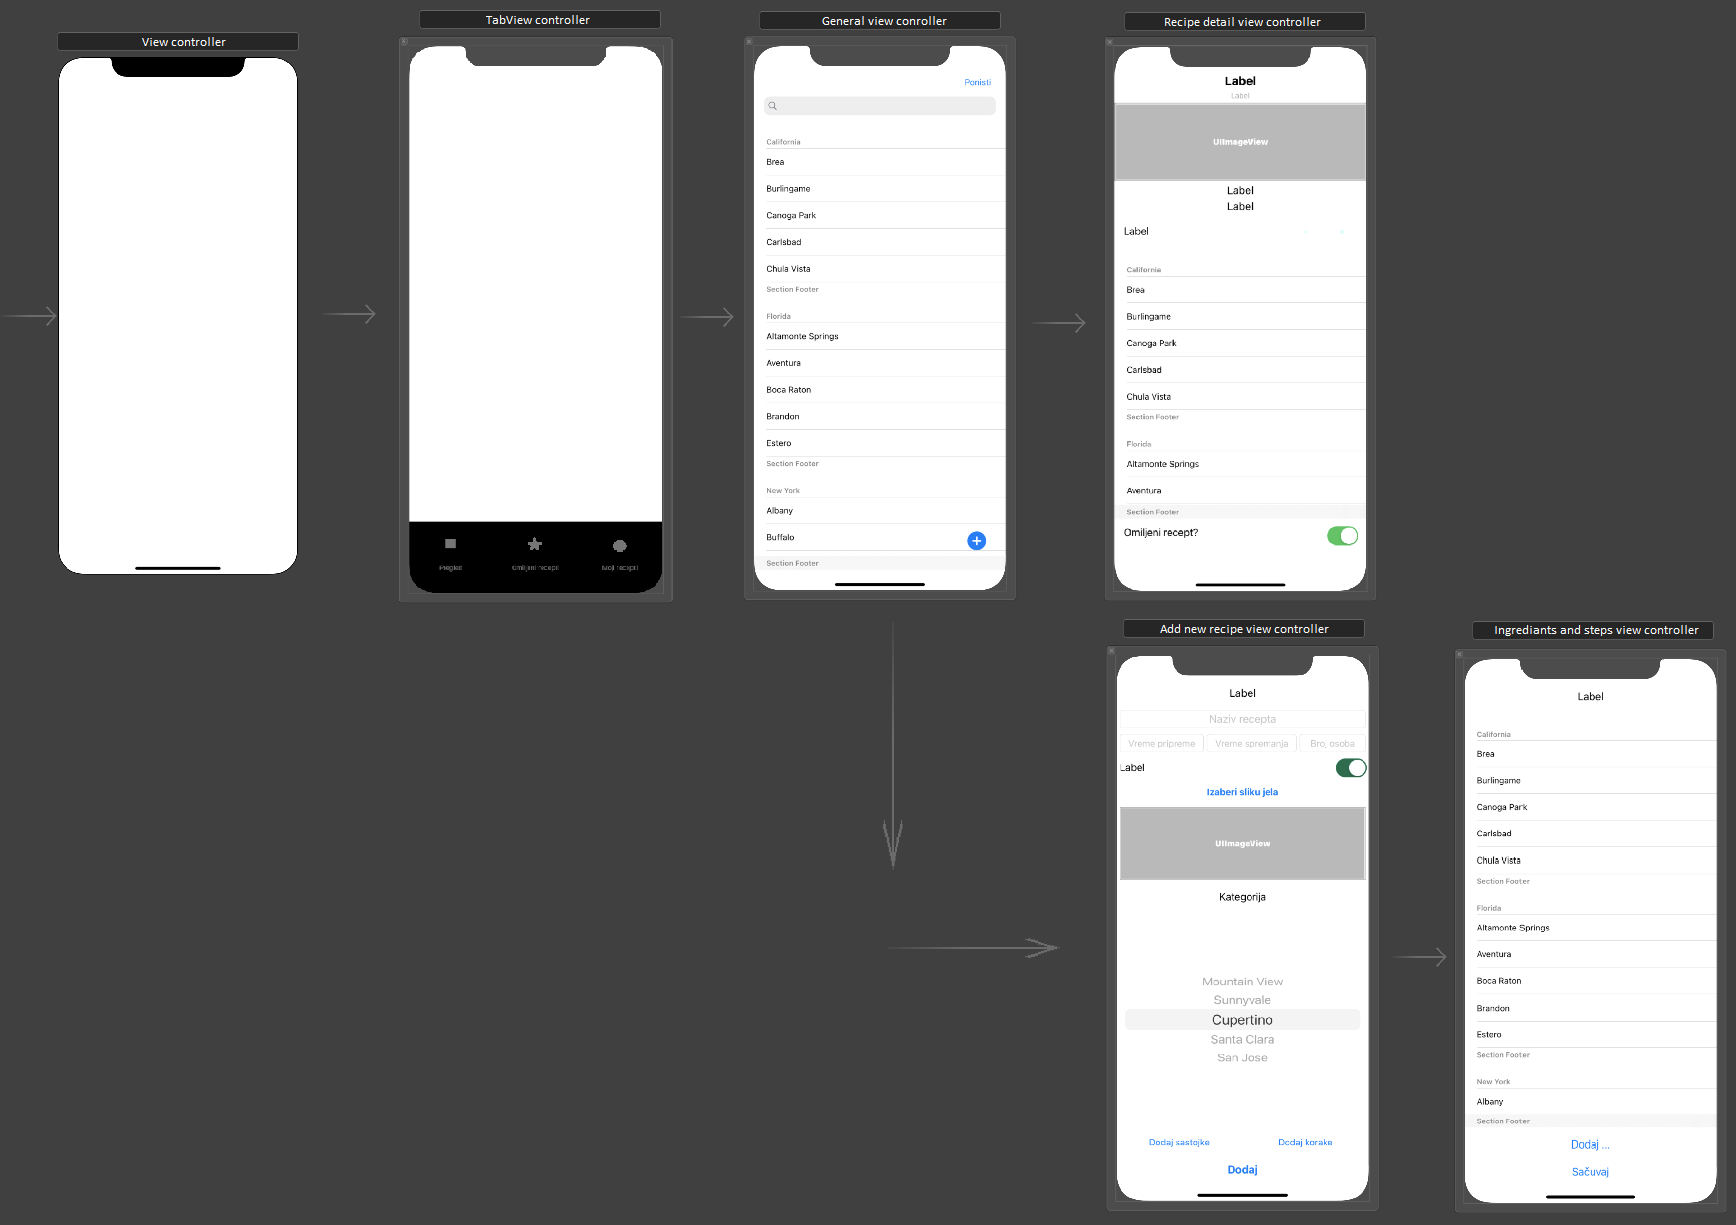
\includegraphics[width=1\textwidth]{images/view_structure.png} 
    \caption{\textit{Структура и повезаност главних погледа}}
    \label{slika:главни_погледи}
\end{figure}

Помоћне погледе чине три погледа који дефинишу изглед ћелија (редова у табели). Први поглед дефинише изглед ћелије приказане у главном прозору, која се састоји од две лабеле (име рецепта и време припреме) и слике рецепта. Други поглед приказује изглед заглавља табеле у главном погледу и садржи лабеле за ознаку имена, времена припреме и слике, док се поред лабеле за ознаку времена припреме налази и дугме за сортирање листе рецепата по времену припреме (растуће и опадајуће). Поседњи помоћни поглед дефинише изглед ћелије унутар табеле приликом додавања или измене састојака или корака припреме рецепта од стране корисника. Приказ изгледа ових ћелија може се видети на слици \ref{slika:помоћни_погледи}.

\begin{figure} [H]
    \centering
    \captionsetup{justification=centering}
    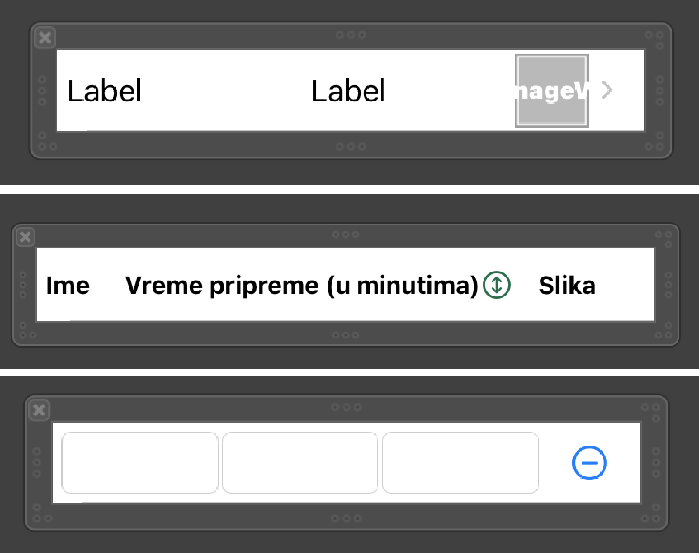
\includegraphics[width=0.5\textwidth]{images/helper_views.png} 
    \caption{\textit{Изглед помоћних погледа}}
    \label{slika:помоћни_погледи}
\end{figure}

\subsection{Имплементација контролера}

Сваки главни поглед има упарени контролер који реагује на интеракцију корисника са апликацијом, обрађује догађај и на основу логике која је имплементирана унутар контролера, ажурира модел и/или одговарајући поглед. Главни контролер је \textit{TabBarViewController}, он одређује која инстанца класе \textit{GeneralViewController} ће бити приказана (преглед, омиљени рецепти или моји рецепти). Ове инстанце се разликују на основу два поља \textit{isFavorites} и \textit{isMyRecipes}. Поред ових поља, класа \textit{GeneralViewController} садржи листе са рецептима које се приказују на основу интеракције корисника са апликацијом. 
Контролер \textit{RecipeDetailViewController} је задужен за поглед који приказује детаљан опис рецепта. Овај контролер омогућава кориснику да повећа или смањи број особа за које ће рецепт бити намењен, чиме ће се аутоматски променити и остали приказани параметри. Количина потребних састојака се мења пропорцијално броју особа, време припреме се мења у односу на фактор времена припреме (променљива која опада или расте логаритамски у односу на тренутни број особа), време кувања се повећава када број особа буде седам и поново када буде петнаест јер се, на пример, време кувања за четири и шест особа не разликује. Унутар погледа корисник може тренутни рецепт додати или избацити из листе омиљених рецепата, док уколико је корисник додао тренутни рецепт, може га изменити или обрисати.

Уколико корисник изабере да дода нови рецепт или измени постојећи, приказаће му се поглед \textit{AddNewRecipeViewController}. Логика која раздваја ова два случаја је имплементирана у контролеру коришћењем променљиве \textit{existingRecipe} типа \textit{Recipe?} и у случају додавања новог рецепта има вредност \textit{nil} и сва приказана поља ће бити попуњена чуварима места (енг. \textit{placeholders}), док у случају измене постојећег рецепта променљива \textit{existingRecipe} ће имати вредност инстаце класе \textit{Recipe} чија ће поља садржати информације о тренутном рецепту и оне ће бити приказане приликом измене рецепта. У случају да корисник жели да дода или измени састојке или кораке припреме рецепта, приказаће му се поглед \textit{IngrediantsStepsViewController}. У зависности да ли корисник додаје рецепт или га мења, контролер \textit{IngrediantsStepsView Controller} ће приказати три празна поља за кораке или састојке приликом додавања рецепта, односно тренутне кораке или састојке у случају измене рецепта. Контролер пружа могућност додавања нових корака и састојака, као и брисање или измену постојећих.

\subsection{Опис имплементације виџета}

У пројекту су имплементирана два типа виџета. Први тип је конфигурабилан и омогућава кориснику да промени рецепт који ће бити приказан као и да изабере главни параметар (састојке или кораке припреме), док други тип приказује насумично изабране рецепте из корисникове листе омиљених рецепата.

Први тип виџета имплементира протокол \textit{IntentTimelineProvider}, чиме се омогућава конфигурација виџета од стране корисника. Избор главног параметра је имплементиран унутар фајла \textit{Intent} у којем су кроз набрајање (енг. \textit{enumeration}) одређене могуће вредности параметра (састојци и припрема). Избор рецепта је такође имплементиран кроз \textit{Intent} фајл, а да би се кориснику омогућио динамичан избор рецепта (избор из тренутне листе омиљених рецепата) апликација је проширена додатком \textit{Intent} унутар ког је имплементирана метода која фајлу \textit{Intent} прослеђује корисникову листу омиљених рецепата. Овај тип виџета је имплементиран у све три величине. Мала величина приказује слику и назив рецепта, средња величина додатно приказује састојке или кораке припреме у зависности који је параметар корисник изабрао као примарни. Велики виџет приказује обе листе (састојке и кораке припреме) поред слике и назива рецепта.

Други тип виџета је креиран само у великој величини, имплементира протокол \textit{TimelineProvider} и нема конфигурабилане параметре. Виџет приказује четири различита, насумично изабрана рецепта из корисникове листе омиљених рецепата. У случају да корисник има мање од четири рецепта у листи омиљених рецепата, виџет ће приказати подразумевани рецепт.

\section{Визуелни приказ и опис апликације}

\indent Рад апликације ће бити приказан упоредо на два симулатора, \textit{iPhone 13 Pro Max} са тамном бојом позадине и \textit{iPhone SE (2nd generation)} са светлом бојом позадине. Оба симулатора покрећу оперативни систем \textit{iOS 15.0}.

\subsection{Почетни екран}

\indent На почетном екрану корисник може видети преглед свих рецепата који су тренутно доступни у апликацији, сортирати рецепте по времену потребном за њихову припрему (растуће и опадајуће), изабрати категорију рецепата који ће бити приказани, претраживати рецепте по именима као и комбиновати ова својства да би у што краћем времену пронашао жељени рецепт (или жељене рецепте).

\indent Рецепти су приказани унутар табеле, сваки рецепт је презентован именом, временом припреме у минутима и сликом. Приказ почетног екрана може се видети на слици \ref{slika:почетни_екран_1}.

\begin{figure} [H]
    \centering
    \captionsetup{justification=centering}
    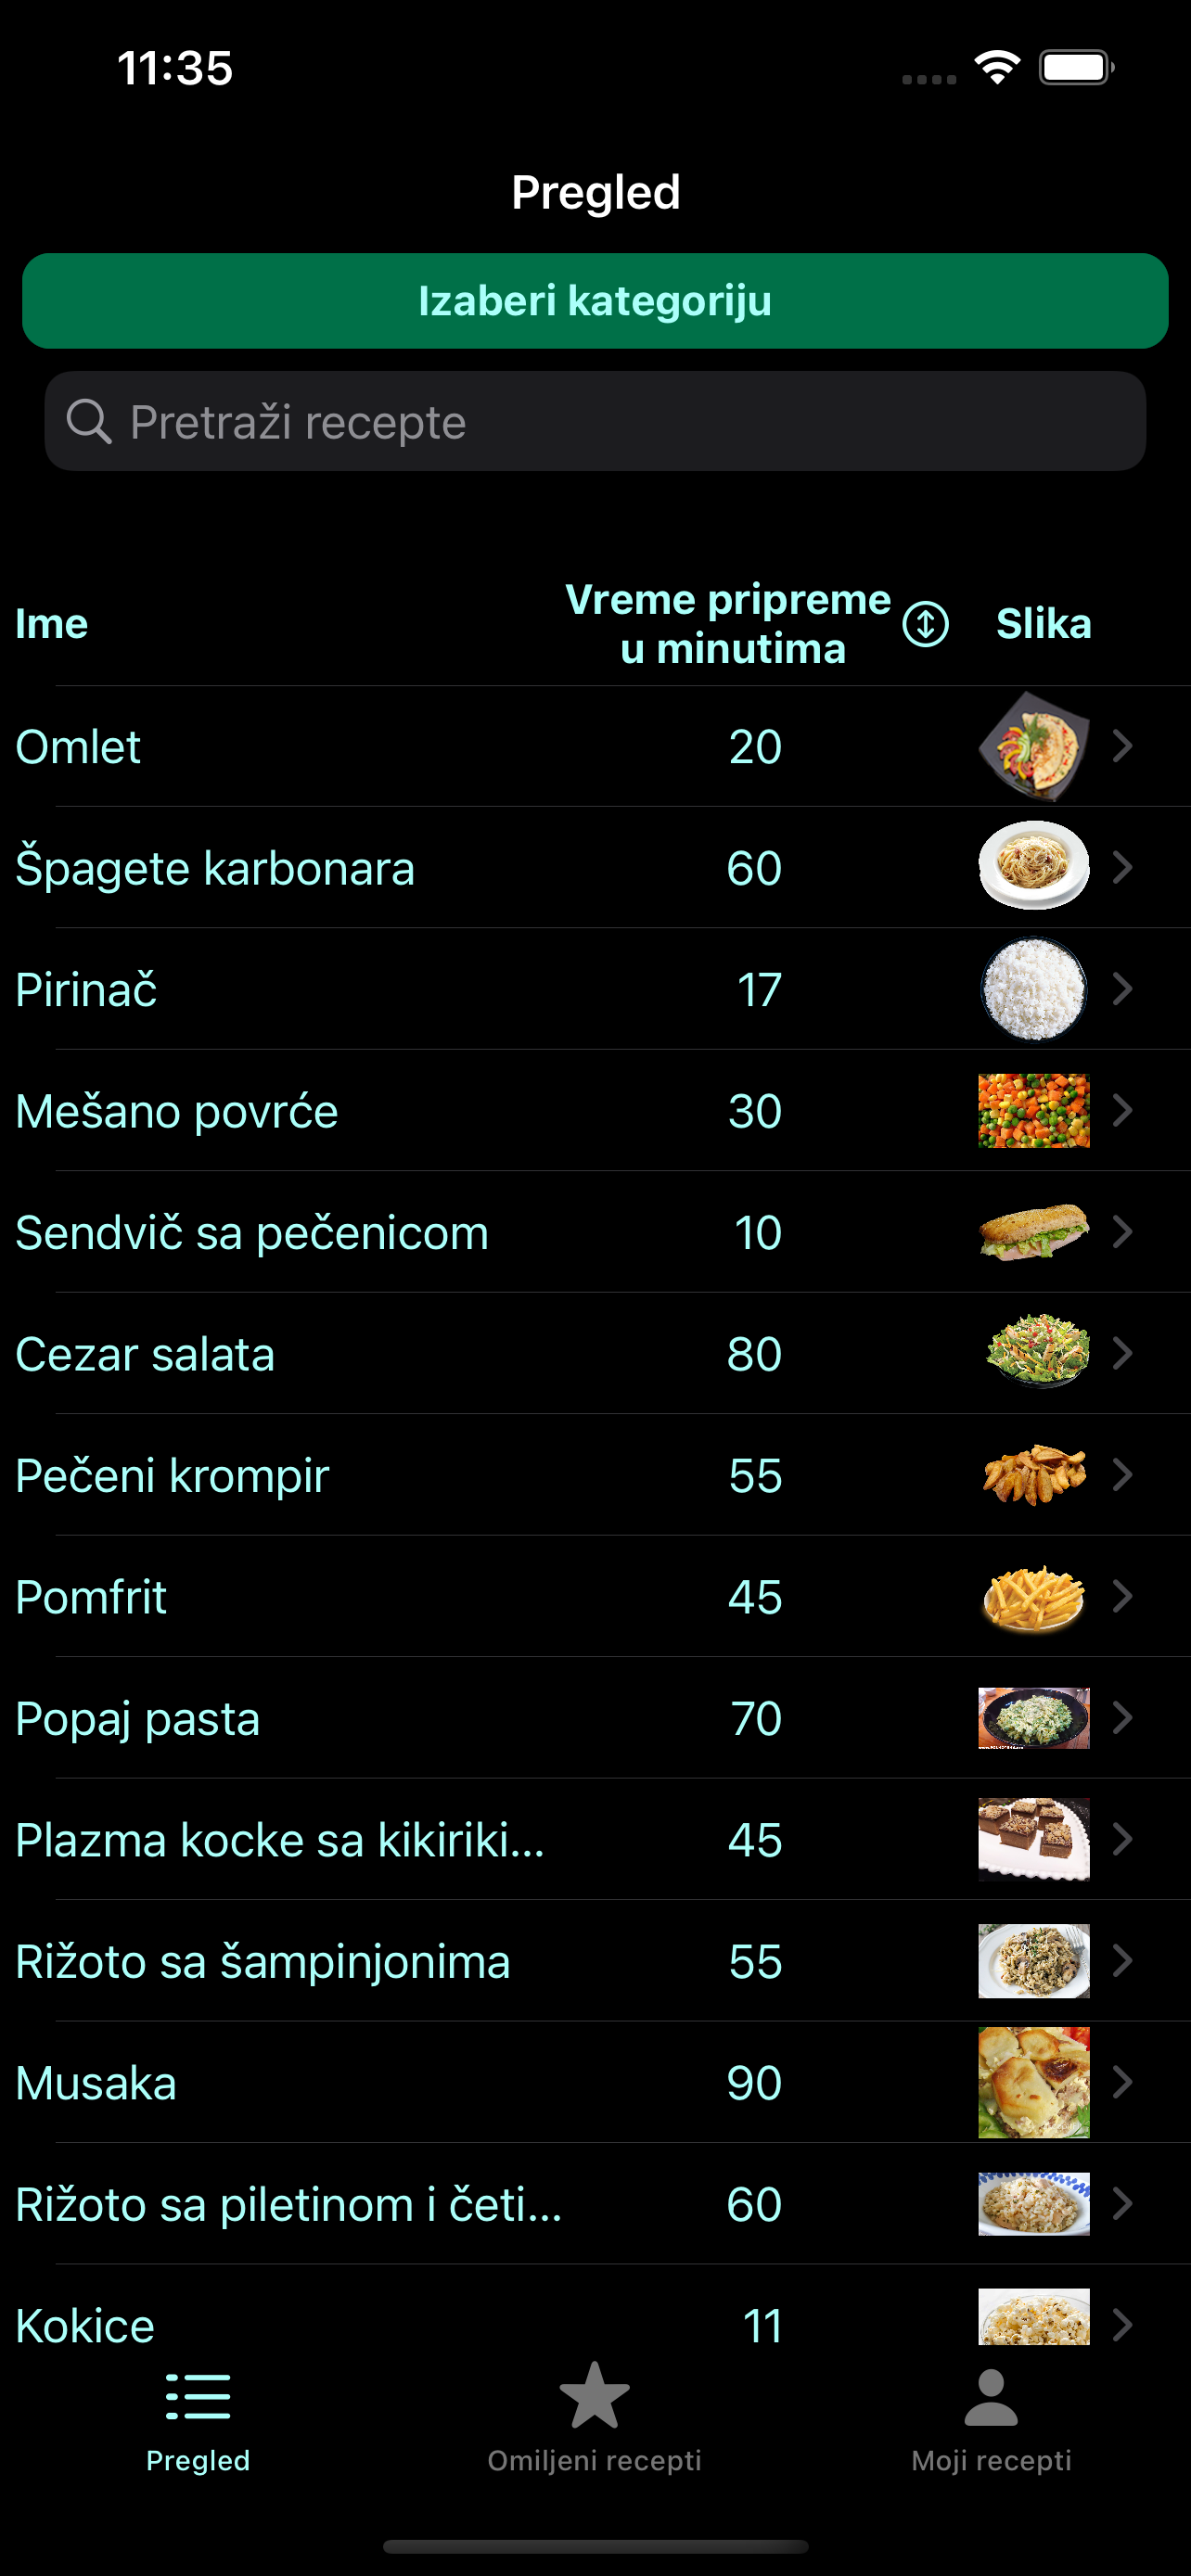
\includegraphics[width=0.475\textwidth]{images/simulators/view images/dark - overview.png} 
    \hfill
    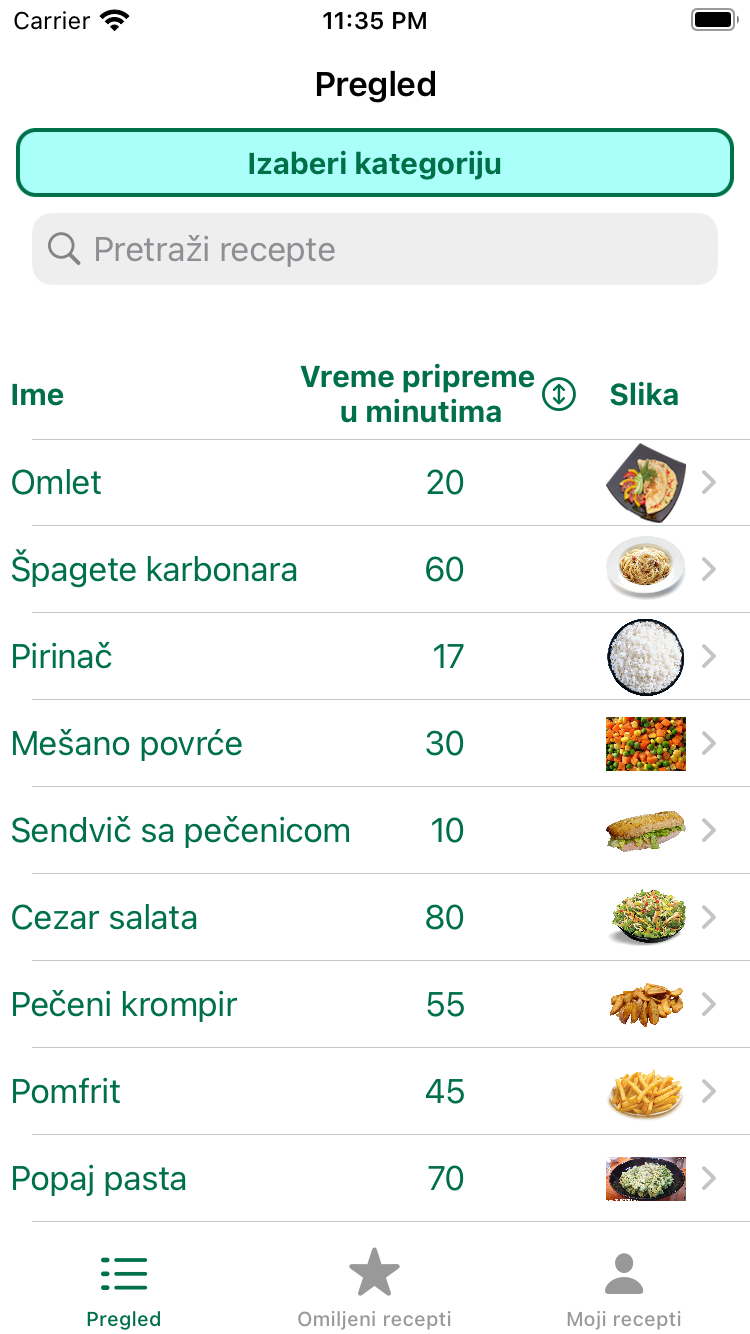
\includegraphics[width=0.475\textwidth]{images/simulators/view images/light - overview.png} 
    \caption{\textit{Почетни екран --- iPhone 13 (лево) и iPhone SE (десно)}}
    \label{slika:почетни_екран_1}
\end{figure}

\indent Корисник може изабрати одређену категорију из које ће му бити приказани рецепти. Међу понуђеним категоријама се налазе "Хладно предјело", "Топло предјело", "Главно јело", "Ужина", "Пиће", "Супе и чорбе", "Дезерт", "Салата" и "Хлеб". Приказ избора категорије налази се на слици \ref{slika:категорија_1}, док је на слици \ref{slika:изабрана_категорија_1} приказан изглед екрана када је једна категорија изабрана (конкретно категорија "Главно јело").

\begin{figure} [H]
    \centering
    \captionsetup{justification=centering}
    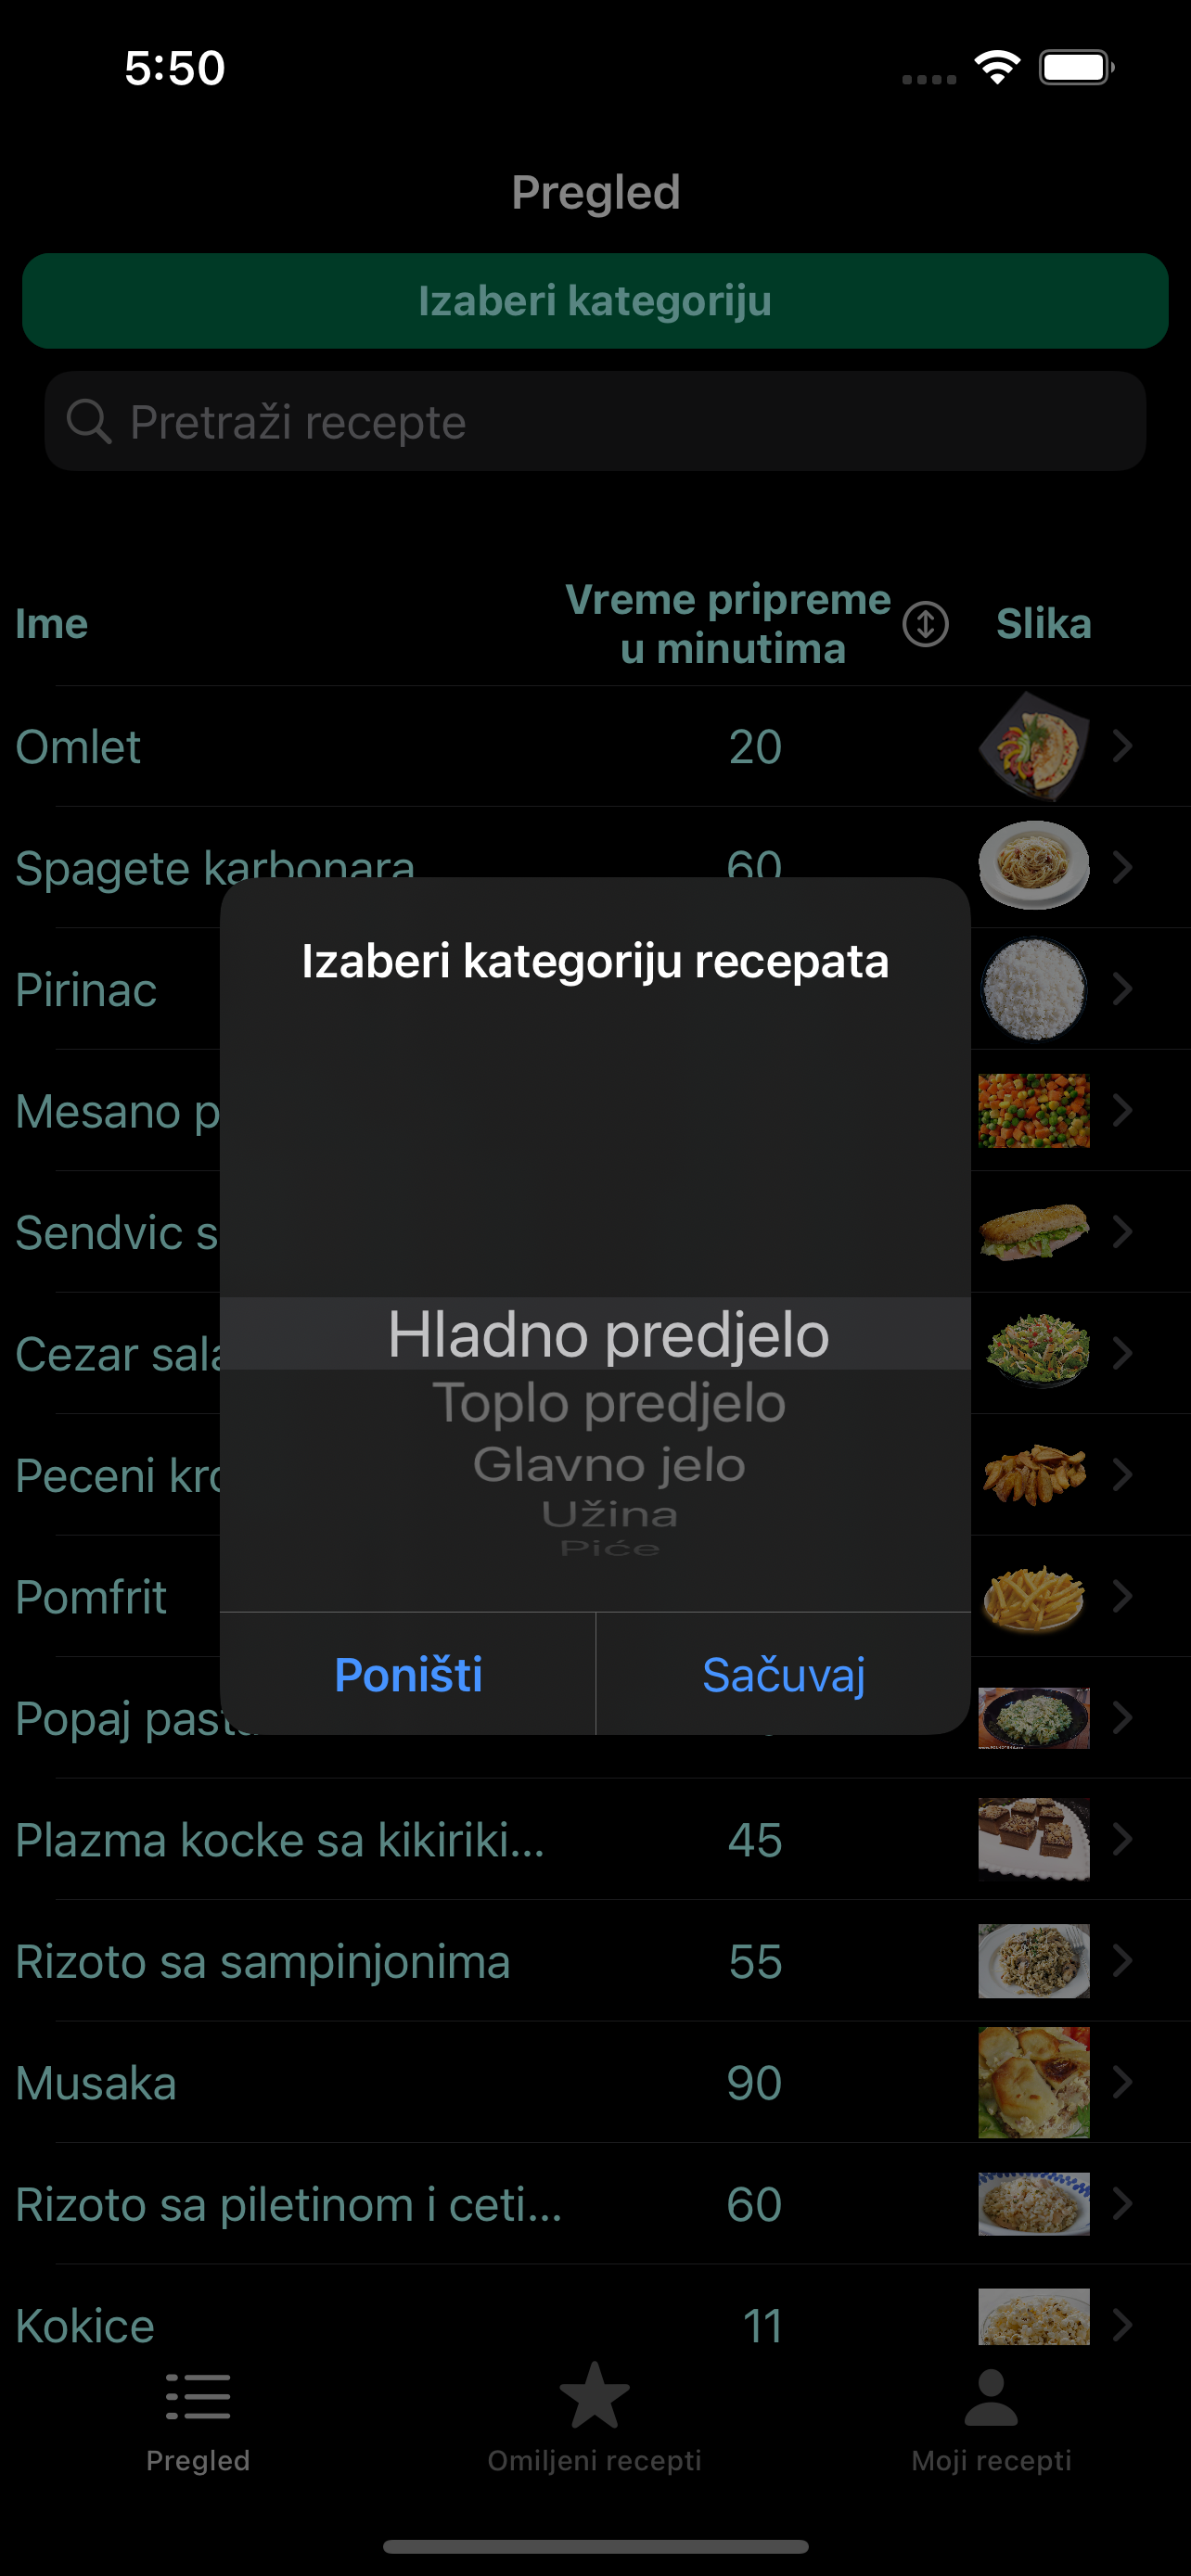
\includegraphics[width=0.475\textwidth]{images/simulators/view images/dark - category.png} 
    \hfill
    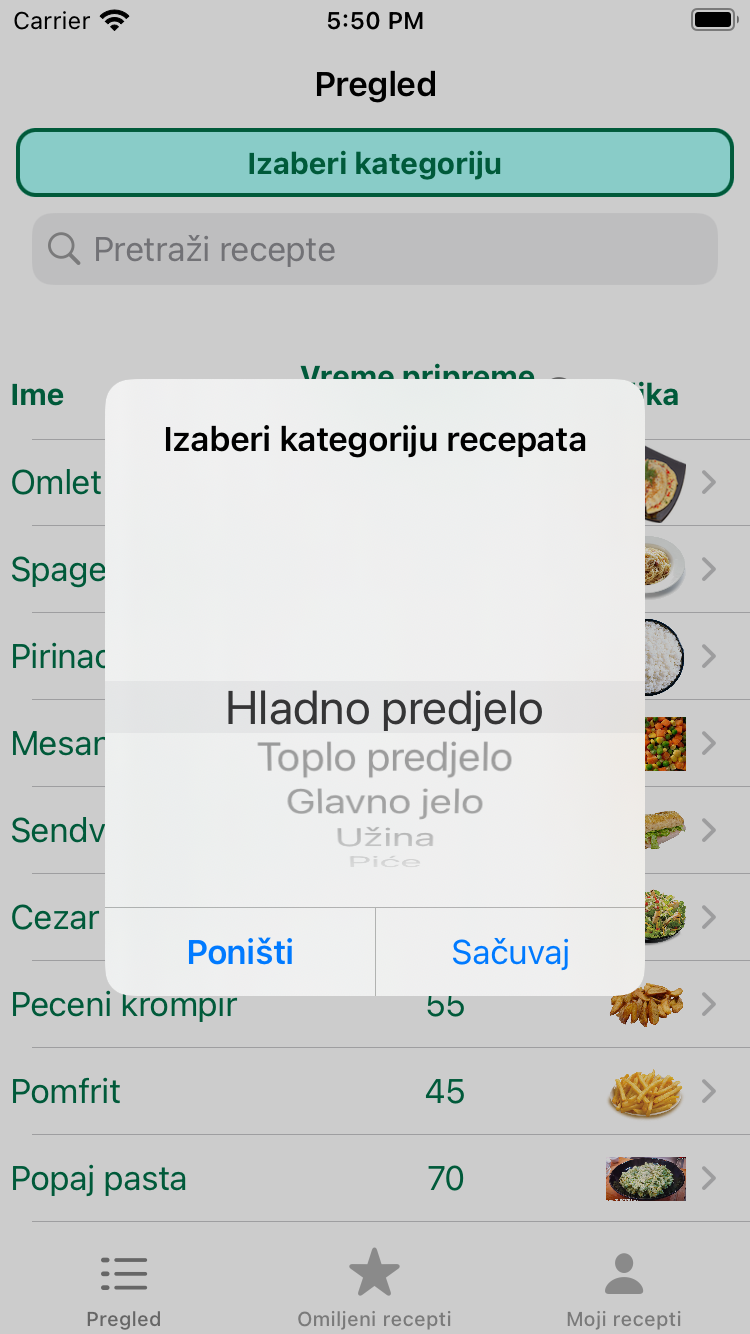
\includegraphics[width=0.475\textwidth]{images/simulators/view images/light - category.png}
    \caption{\textit{Избор категорије --- iPhone 13 (лево) и iPhone SE (десно)}}
    \label{slika:категорија_1}
\end{figure}

\begin{figure} [H]
    \centering
    \captionsetup{justification=centering}
    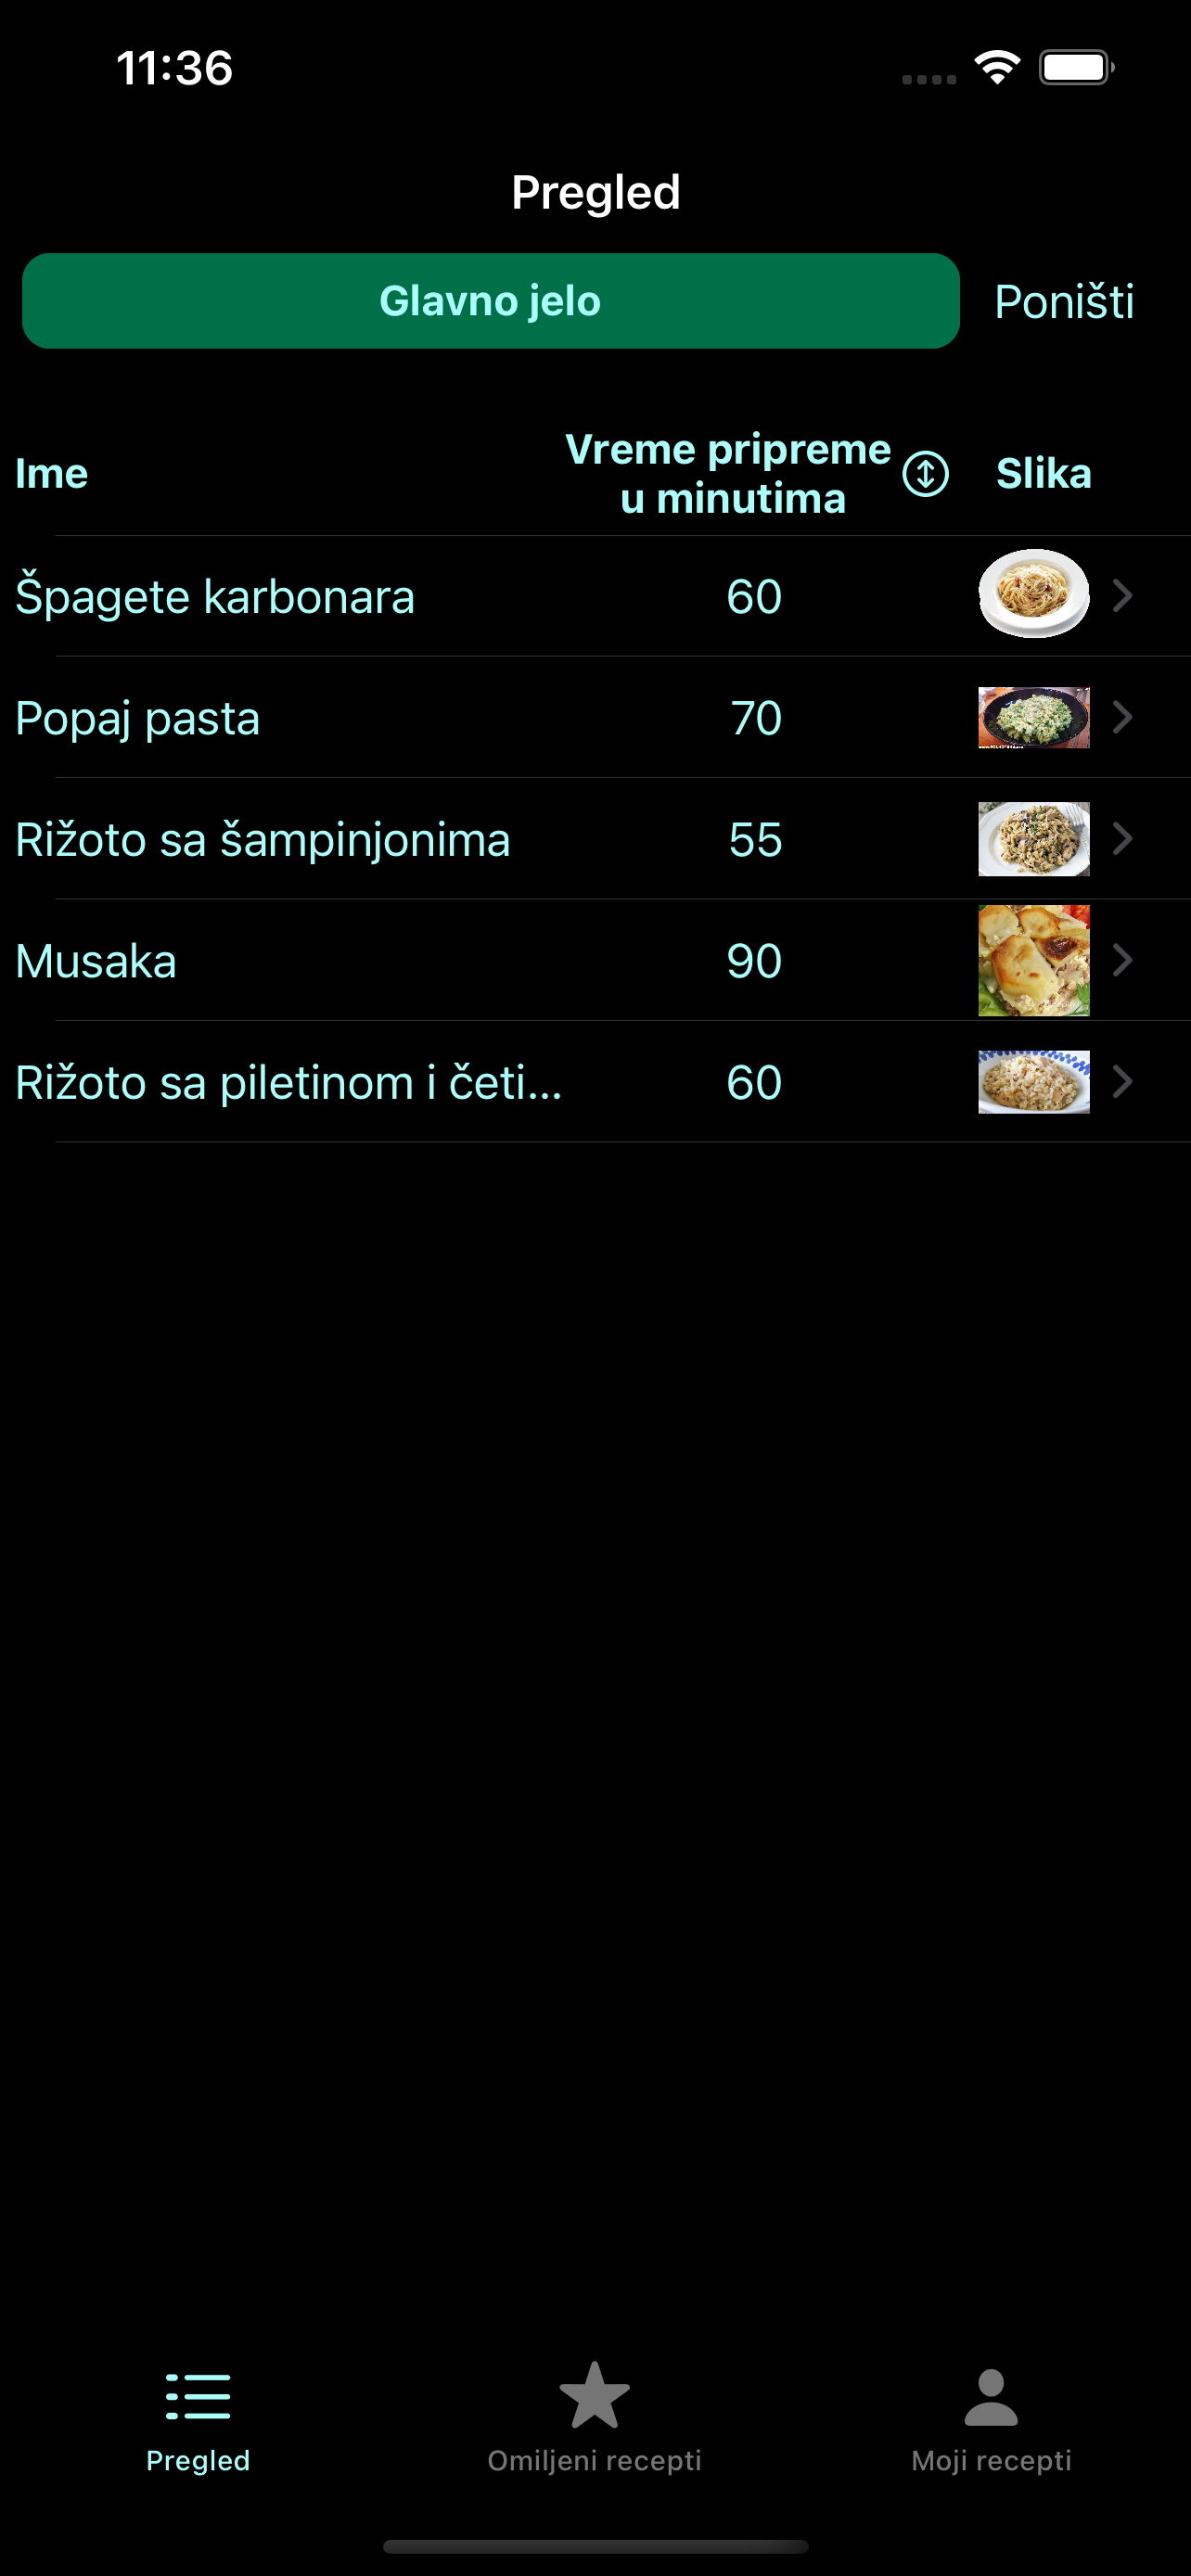
\includegraphics[width=0.475\textwidth]{images/simulators/view images/dark - choosen category.png}
    \hfill
    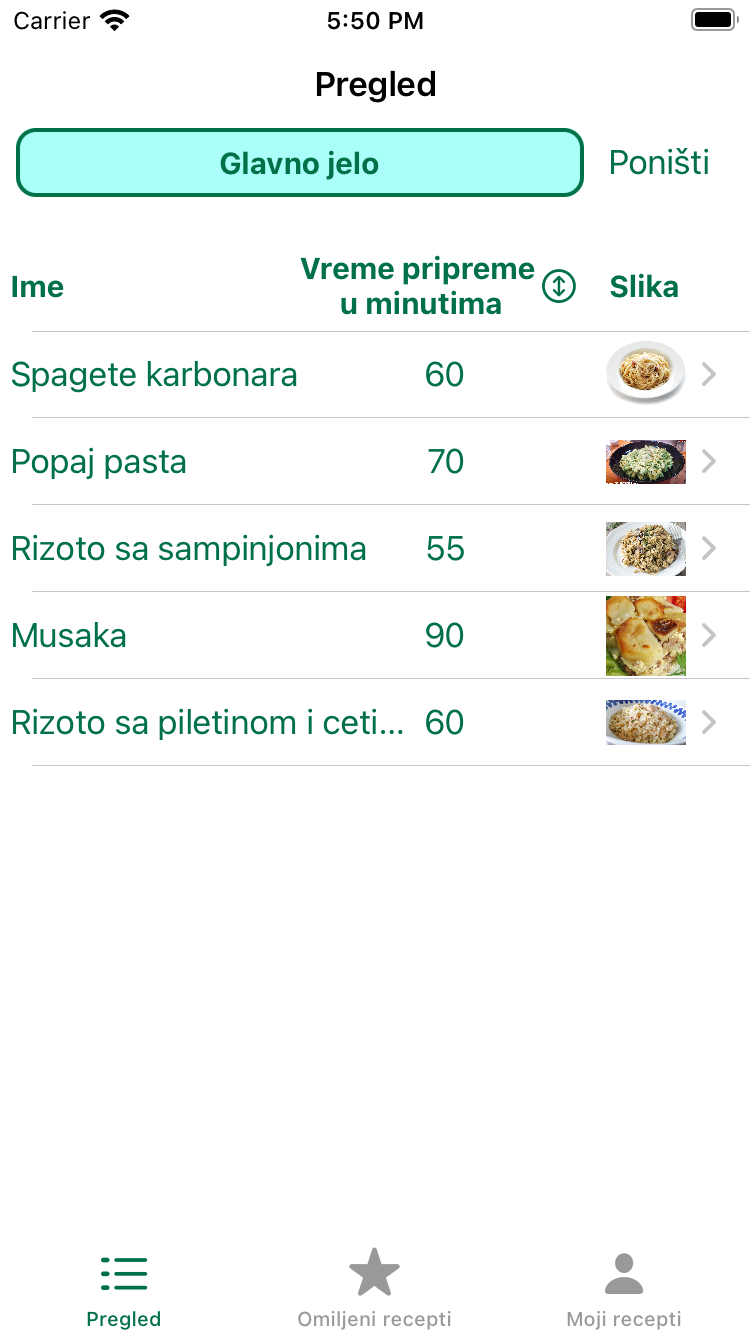
\includegraphics[width=0.475\textwidth]{images/simulators/view images/light - choosen category.png}
    \caption{\textit{Категорија "Главно јело" --- iPhone 13 (лево) и iPhone SE (десно)}}
    \label{slika:изабрана_категорија_1}
\end{figure}

\indent Поред избора категорије, корисник може филтрирати приказане рецепте претрагом по имену и у том случају ће му бити приказани сви рецепти чије име садржи текст који је корисник унео у поље претраге. Почетак претраге приказан је на слици \ref{slika:претрага_1}.

\begin{figure} [H]
    \centering
    \captionsetup{justification=centering}
    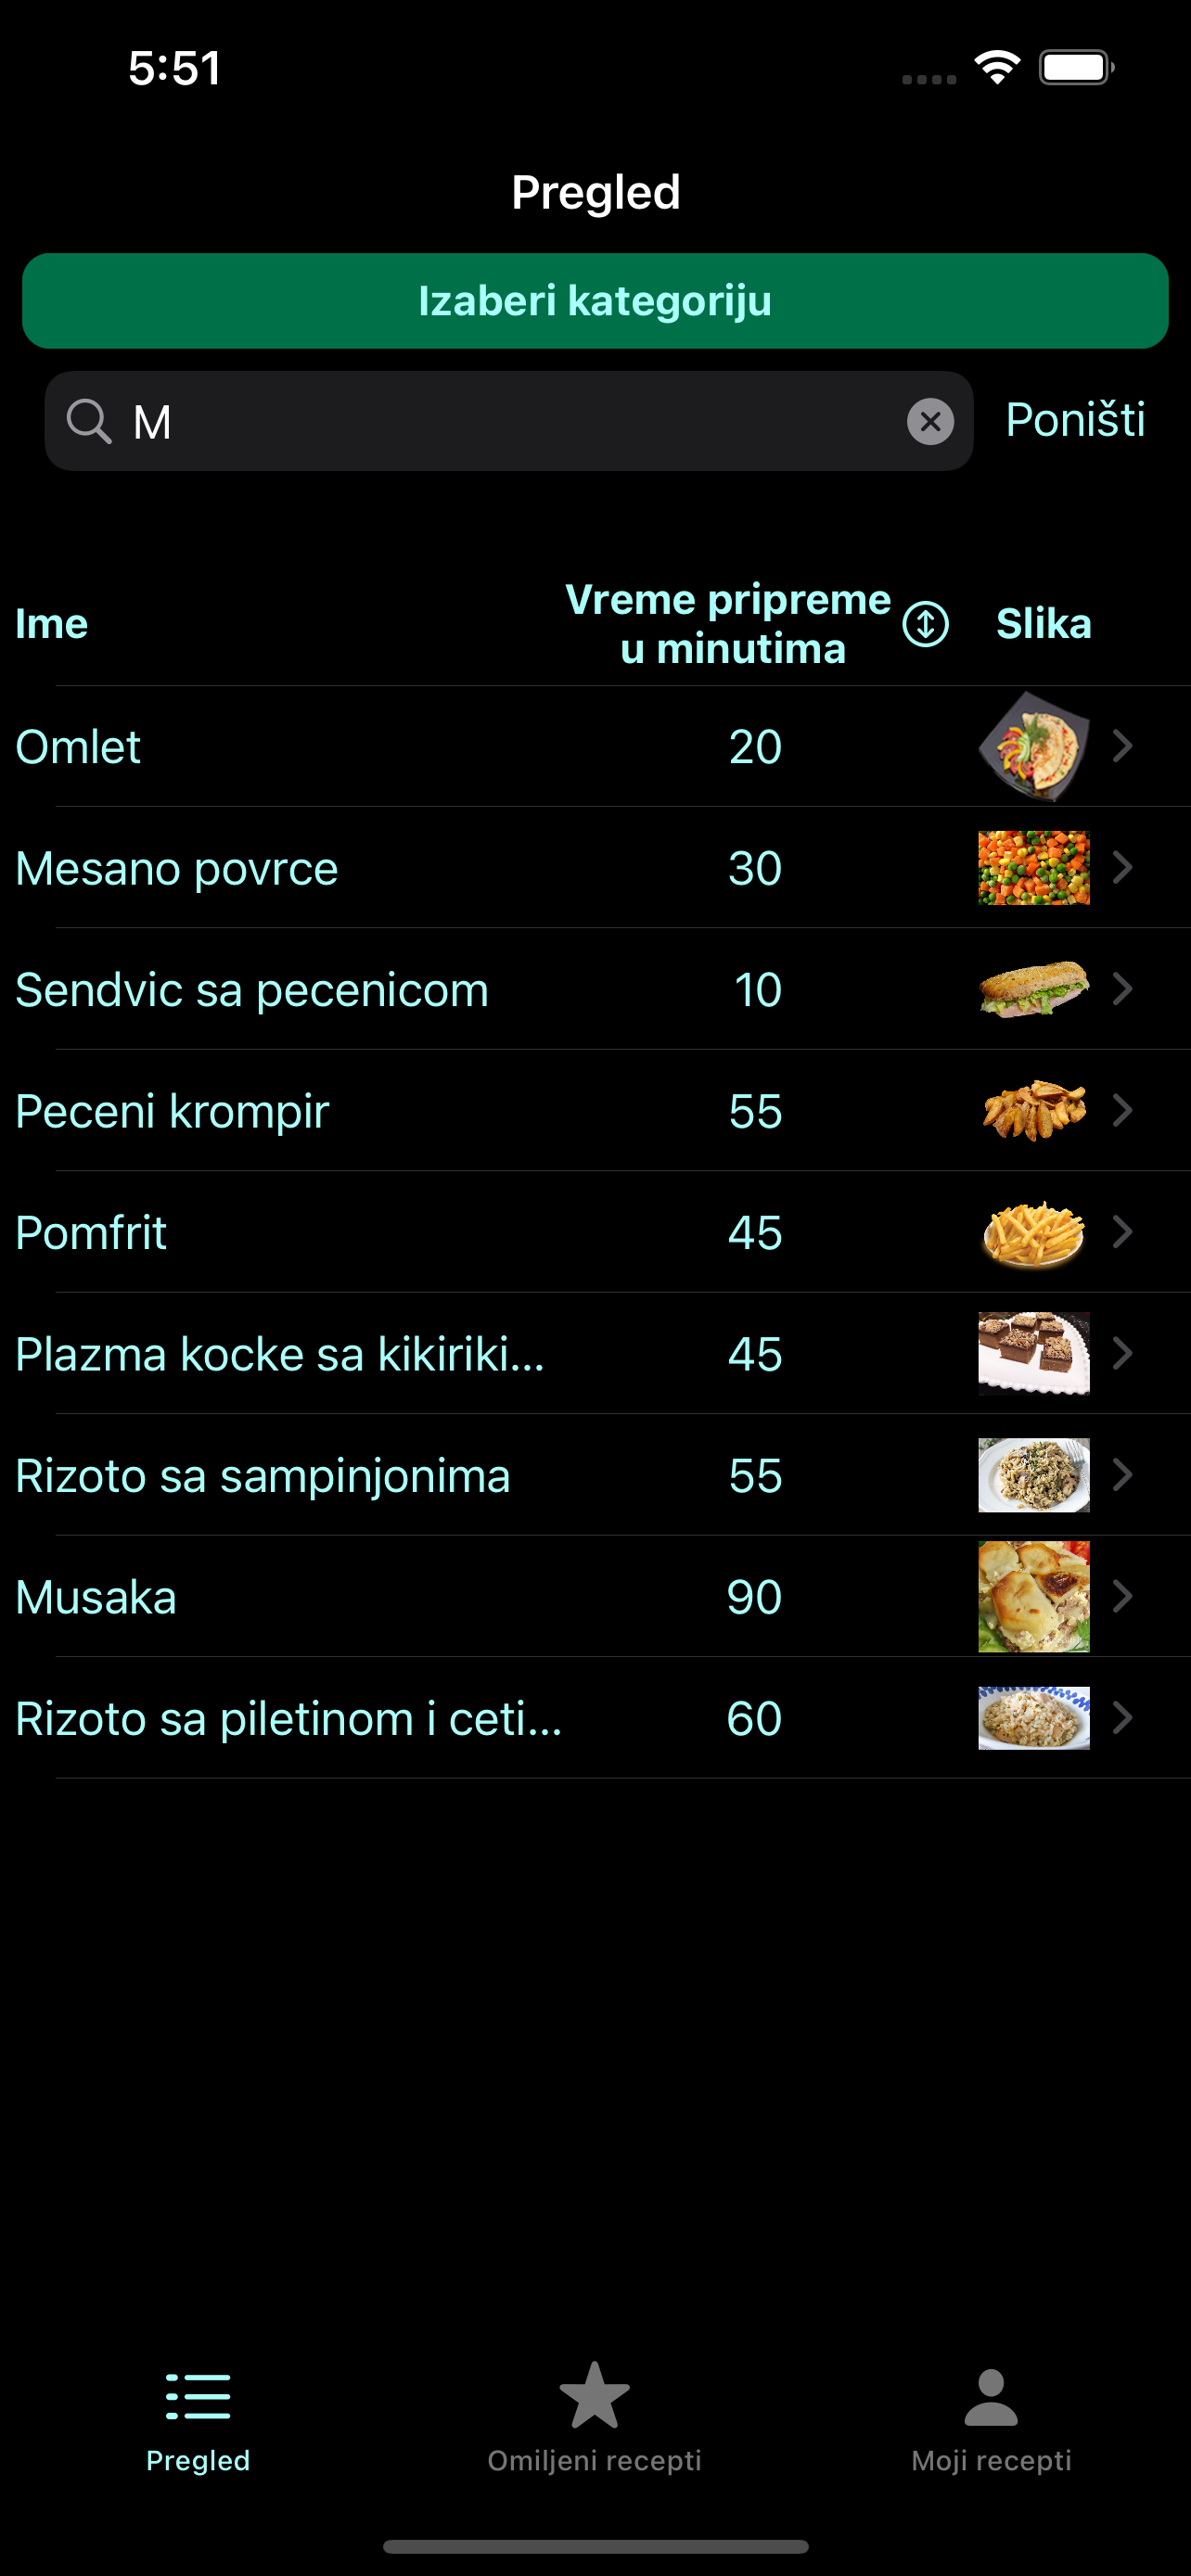
\includegraphics[width=0.475\textwidth]{images/simulators/view images/dark - search.png} 
    \hfill
    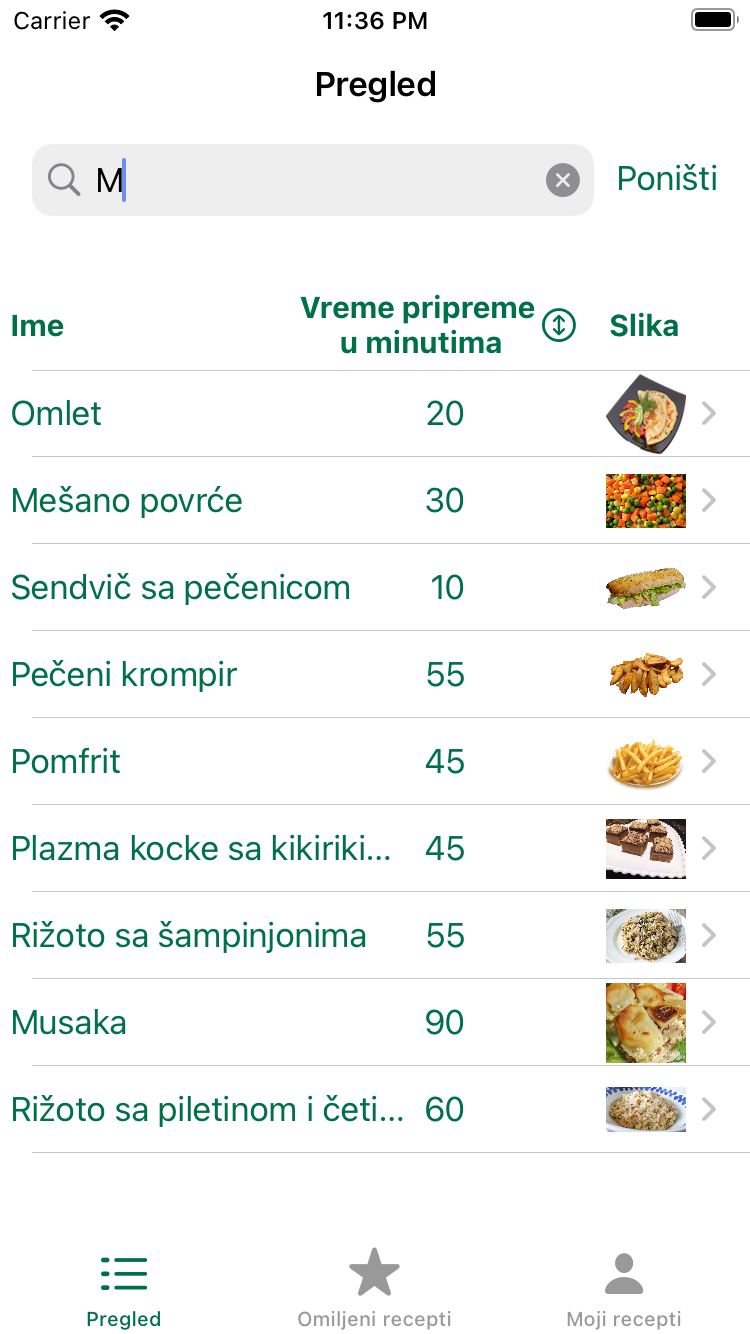
\includegraphics[width=0.475\textwidth]{images/simulators/view images/light - search.png} 
    \caption{\textit{Претрага --- iPhone 13 (лево) и iPhone SE (десно)}}
    \label{slika:претрага_1}
\end{figure}

\indent Рецепте на почетној страни корисник може и сортирати, опадајуће или растуће по укупном времену потребном за њихову припрему (припрема и спремање). Сортирање се може и комбиновати са избором категорије или претрагом по називу, па тако корисник лако може наћи рецепт из одређене категорије (на пример, из категорије дезерта) за чију припрему је потребно издвојити најмање времена. Сортирани рецепти у растућем редоследу су приказани на слици \ref{slika:сортирање_растуће_1}.

\begin{figure} [H]
    \centering
    \captionsetup{justification=centering}
    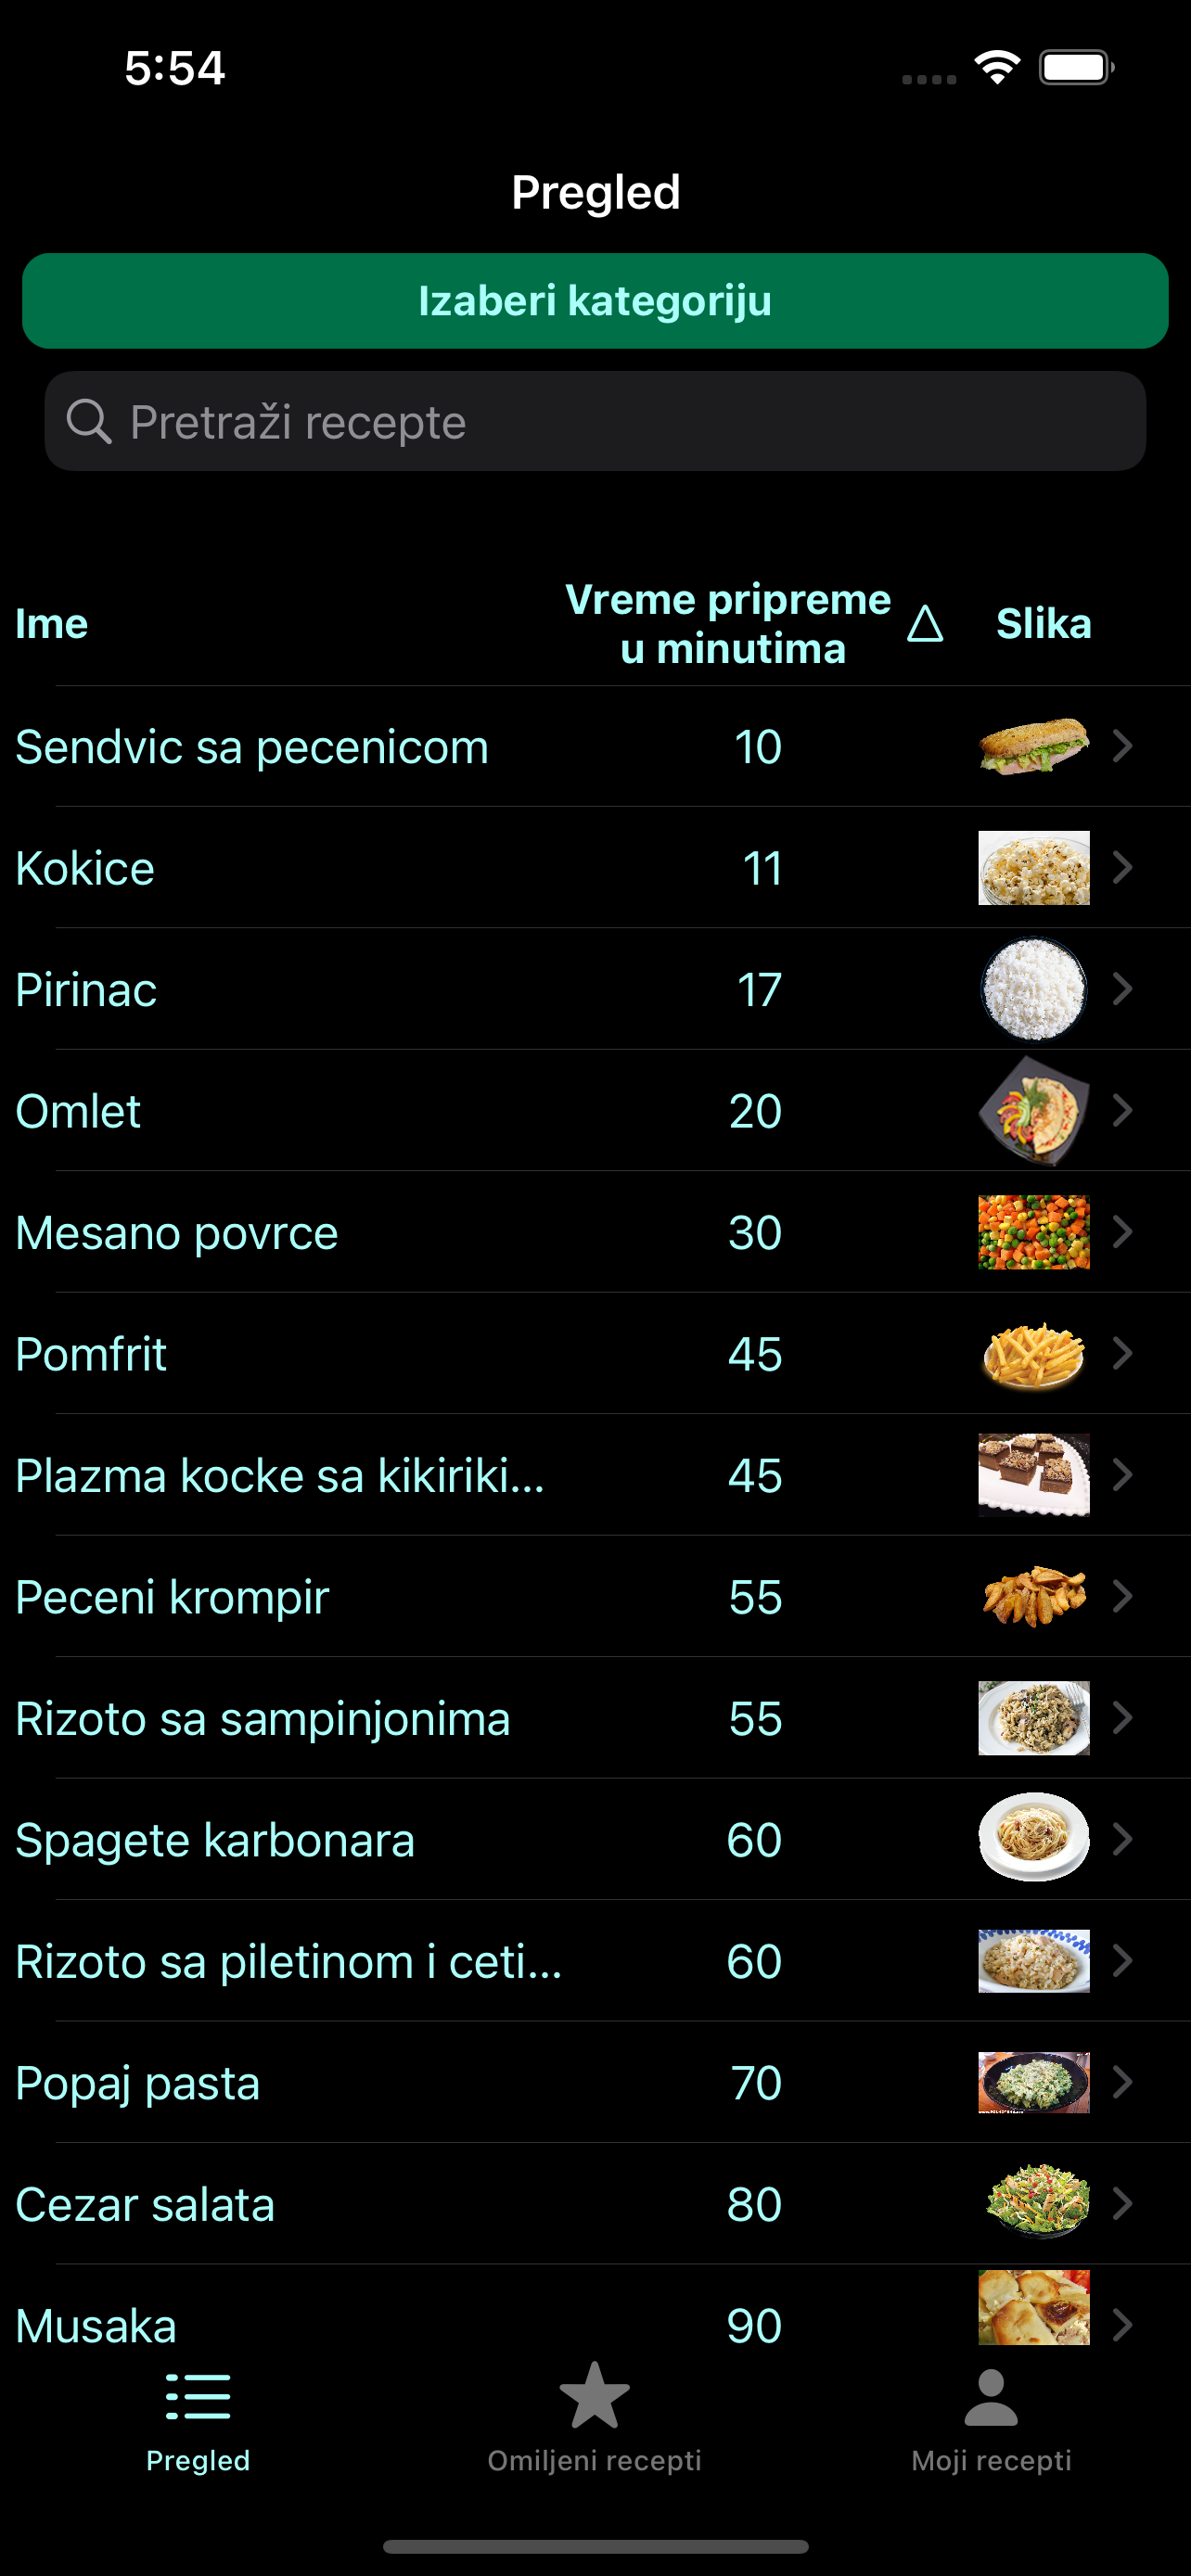
\includegraphics[width=0.475\textwidth]{images/simulators/view images/dark - sort asc.png}
    \hfill
    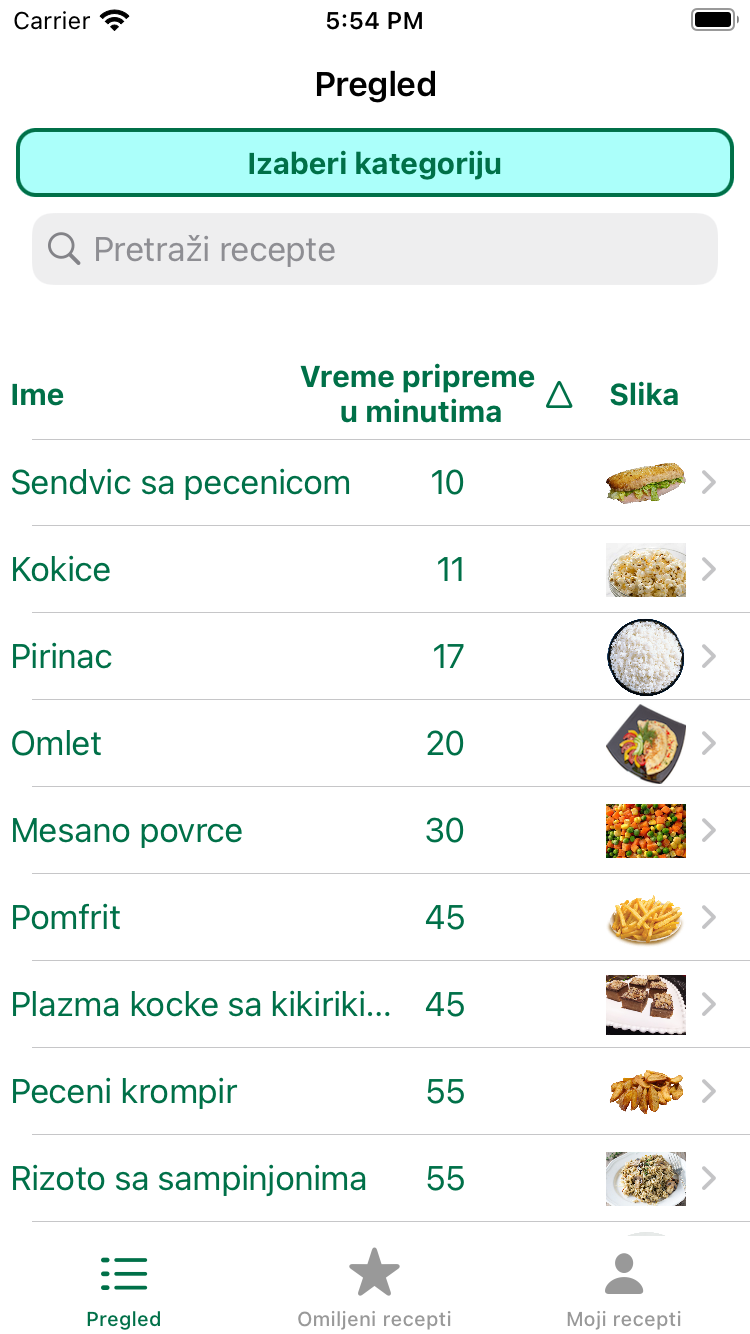
\includegraphics[width=0.475\textwidth]{images/simulators/view images/light - sort asc.png} 
    \caption{\textit{Рецепти сортирани растуће --- iPhone 13 (лево) и iPhone SE (десно)}}
    \label{slika:сортирање_растуће_1}
\end{figure}

\subsection{Омиљени и моји рецепти}

\indent Поред дела са прегледом свих рецепата на почетном екрану, кориснику се пружа могућност прегледа дела "Омиљени рецепти" и "Моји рецепти". Све могућности управљања рецептима (избор категорије, претрага по називу и сортирање) које су кориснику биле на располагању у почетном делу, су омогућене и у преостала два главна дела апликације.

\indent "Омиљени рецепти" је део апликације који садржи листу свих рецепата које је корисник означио као омиљене и тиме их издвојио од осталих. Слика \ref{slika:омиљени_1} представља изглед дела "Омиљени рецепти".

\begin{figure} [H]
    \centering
    \captionsetup{justification=centering}
    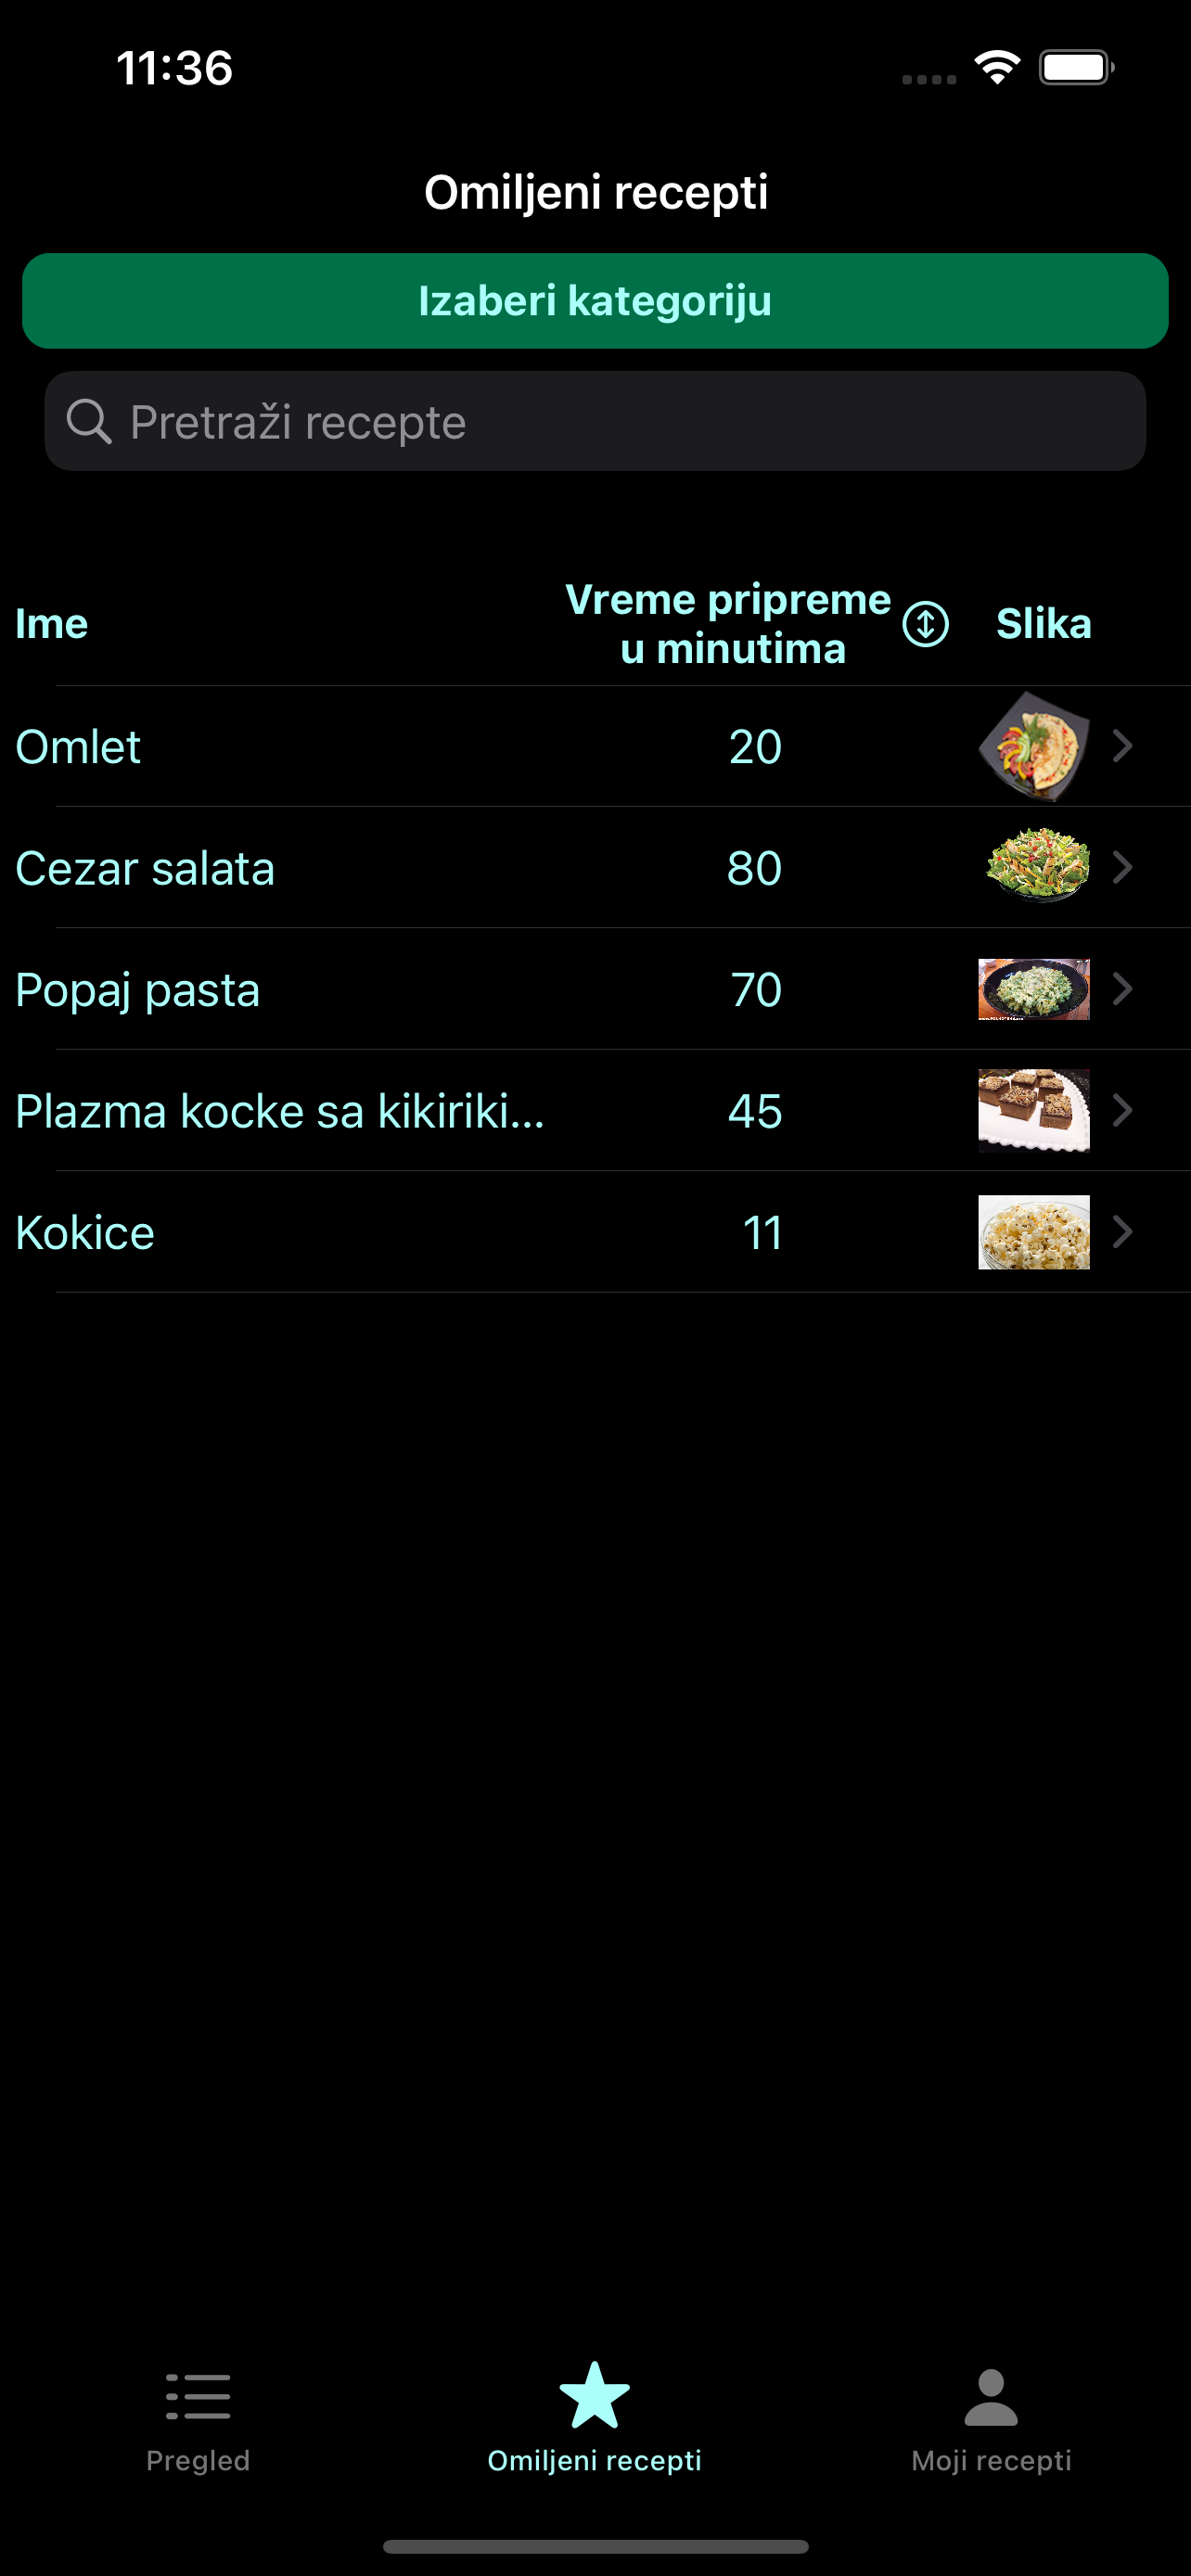
\includegraphics[width=0.475\textwidth]{images/simulators/view images/dark - favorites.png} 
    \hfill
    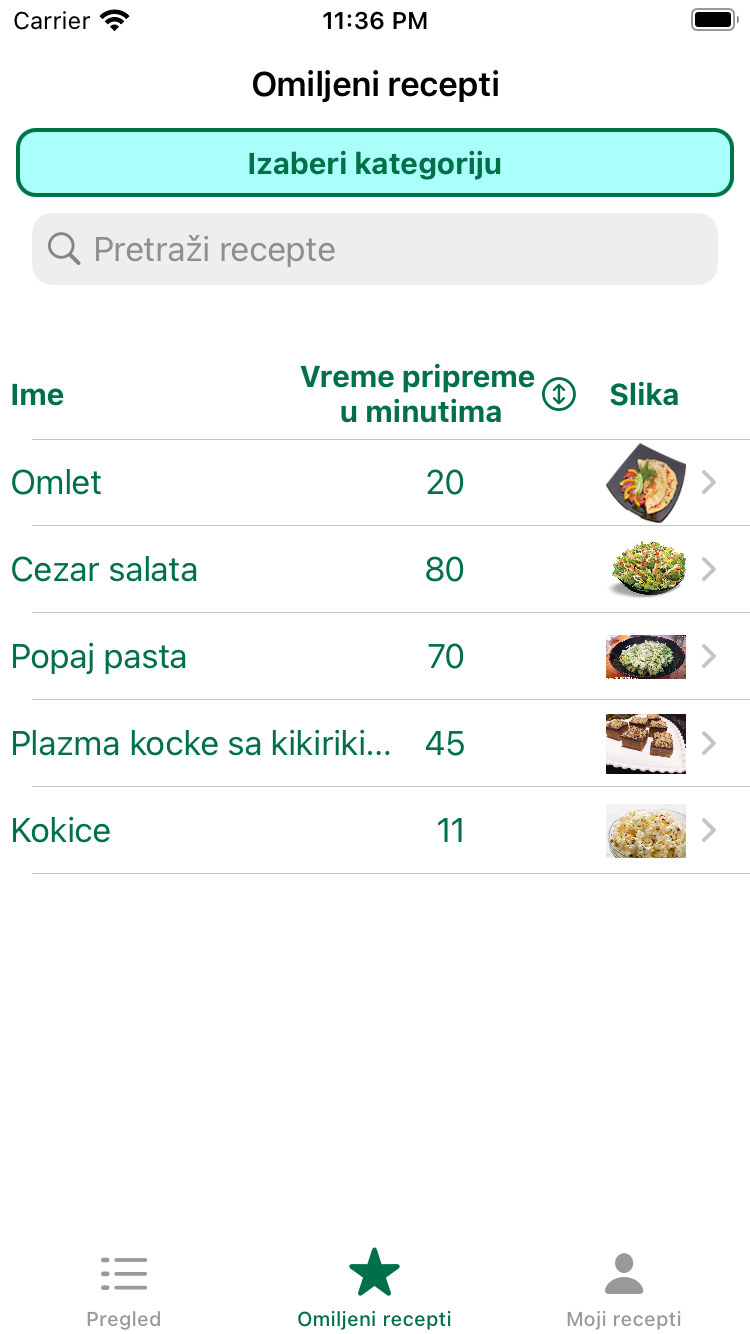
\includegraphics[width=0.475\textwidth]{images/simulators/view images/light - favorites.png}
    \caption{\textit{Омиљени рецепти --- iPhone 13 (лево) и iPhone SE (десно)}}
    \label{slika:омиљени_1}
\end{figure}

\indent Када корисник дода свој рецепт, он ће бити приказан у делу "Моји рецепти" у којем ће корисник моћи да види све своје рецепте са којима може манипулисати, више о овоме биће објашњено у делу \ref{subsec:Измена и брисање постојећег рецепта} --- \nameref{subsec:Измена и брисање постојећег рецепта}. Још једна могућност која се пружа кориснику на овој страни је додавање новог рецета, што ће детаљно бити објашњено у делу \ref{subsec:Креирање новог рецепта} --- \nameref{subsec:Креирање новог рецепта}. Сликом \ref{slika:моји_рецепти_1} приказан је изглед странице "Моји рецепти".

\begin{figure} [H]
    \centering
    \captionsetup{justification=centering}
    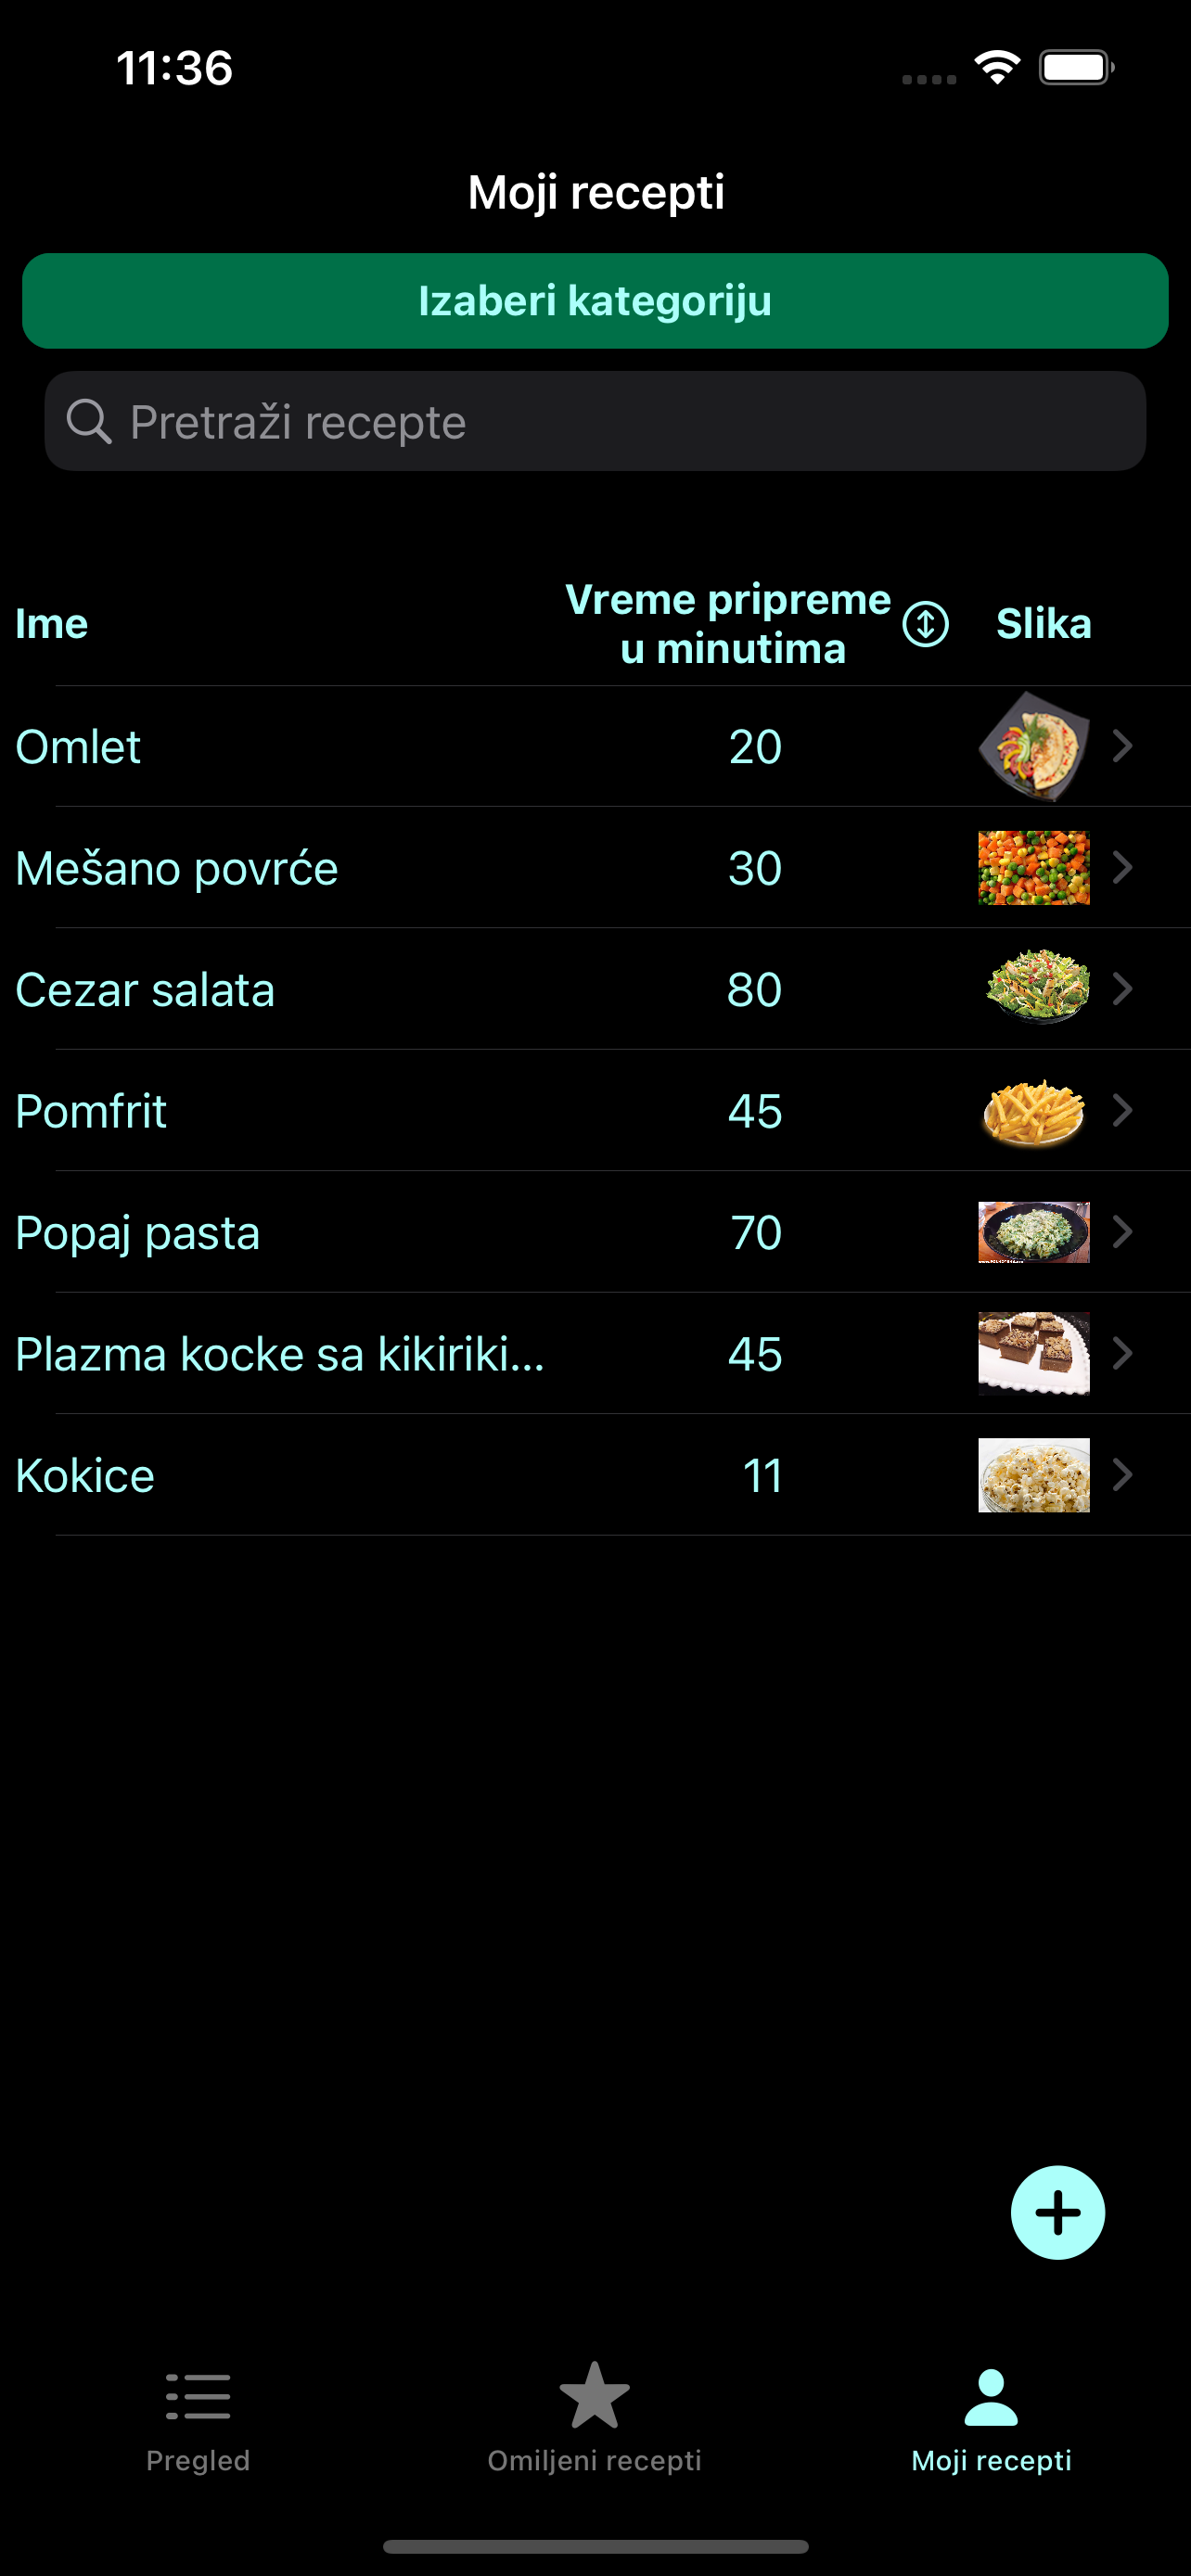
\includegraphics[width=0.475\textwidth]{images/simulators/view images/dark - my recipes.png} 
    \hfill
    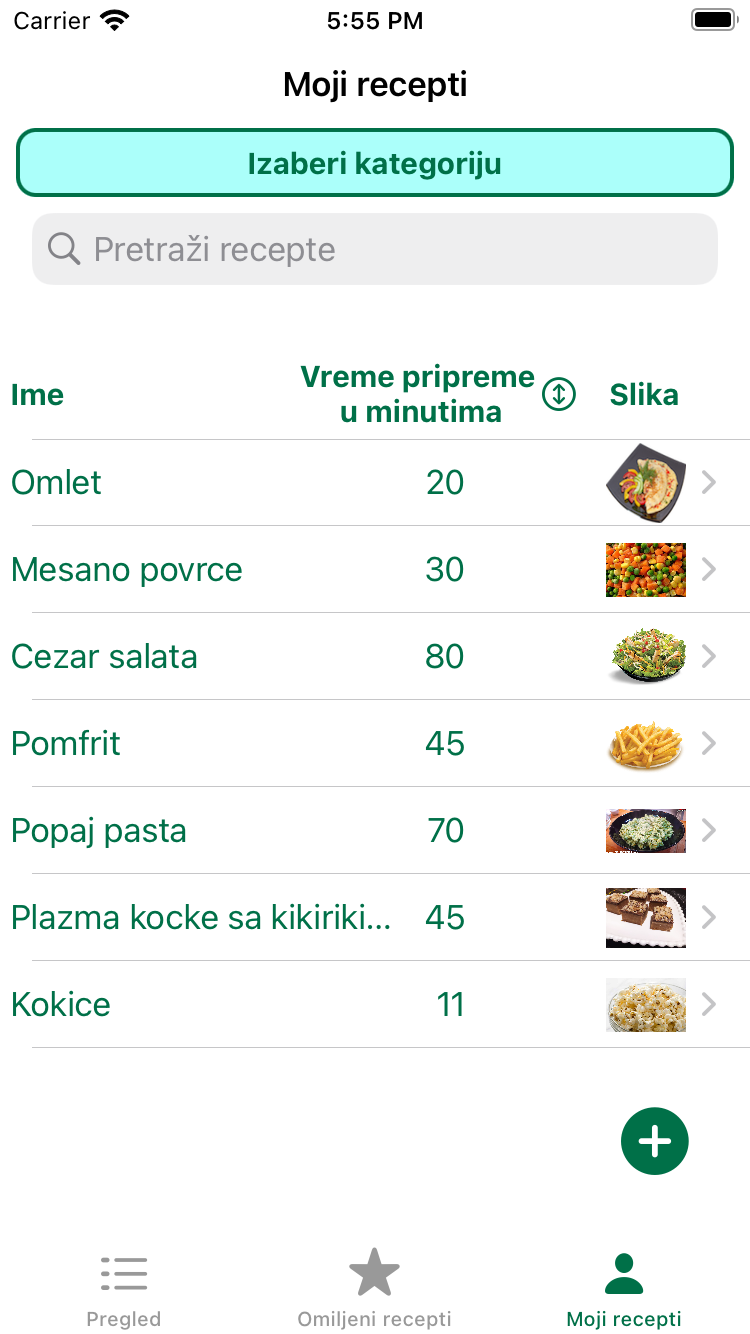
\includegraphics[width=0.475\textwidth]{images/simulators/view images/light - my recipes.png}
    \caption{\textit{Моји рецепти --- iPhone 13 (лево) и iPhone SE (десно)}}
    \label{slika:моји_рецепти_1}
\end{figure}

\subsection{Детаљан приказ рецепта}
\label{subsec:детаљан_рецепт}

\indent У детаљном приказу рецепта, кориснику је презентован опис рецепта који се састоји од: назива рецепта, категорије којој рецепт припада, слике рецепта, времена припреме и спремања, броја особа за које је приказана количина састојака намењена, списка састојака и корака припреме, као и могућности додавања и брисања рецепта из листе омиљених рецепата. Кориснику се пружа могућност повећавања и смањивања броја особа за које је рецепт предвиђен (истовремено ће бити промењена количина састојака као и време припреме). Уколико је приказани рецепт креиран од стране тренутног корисника, приказана су два дугмета за измену и брисање рецепта. Детаљан приказ рецепта за Цезар салату представљен је на слици \ref{slika:детаљан_рецепт_1} за четири особе, односно на слици \ref{slika:детаљан_рецепт_2_1} за шест особа.

\begin{figure} [H]
    \centering
    \captionsetup{justification=centering}
    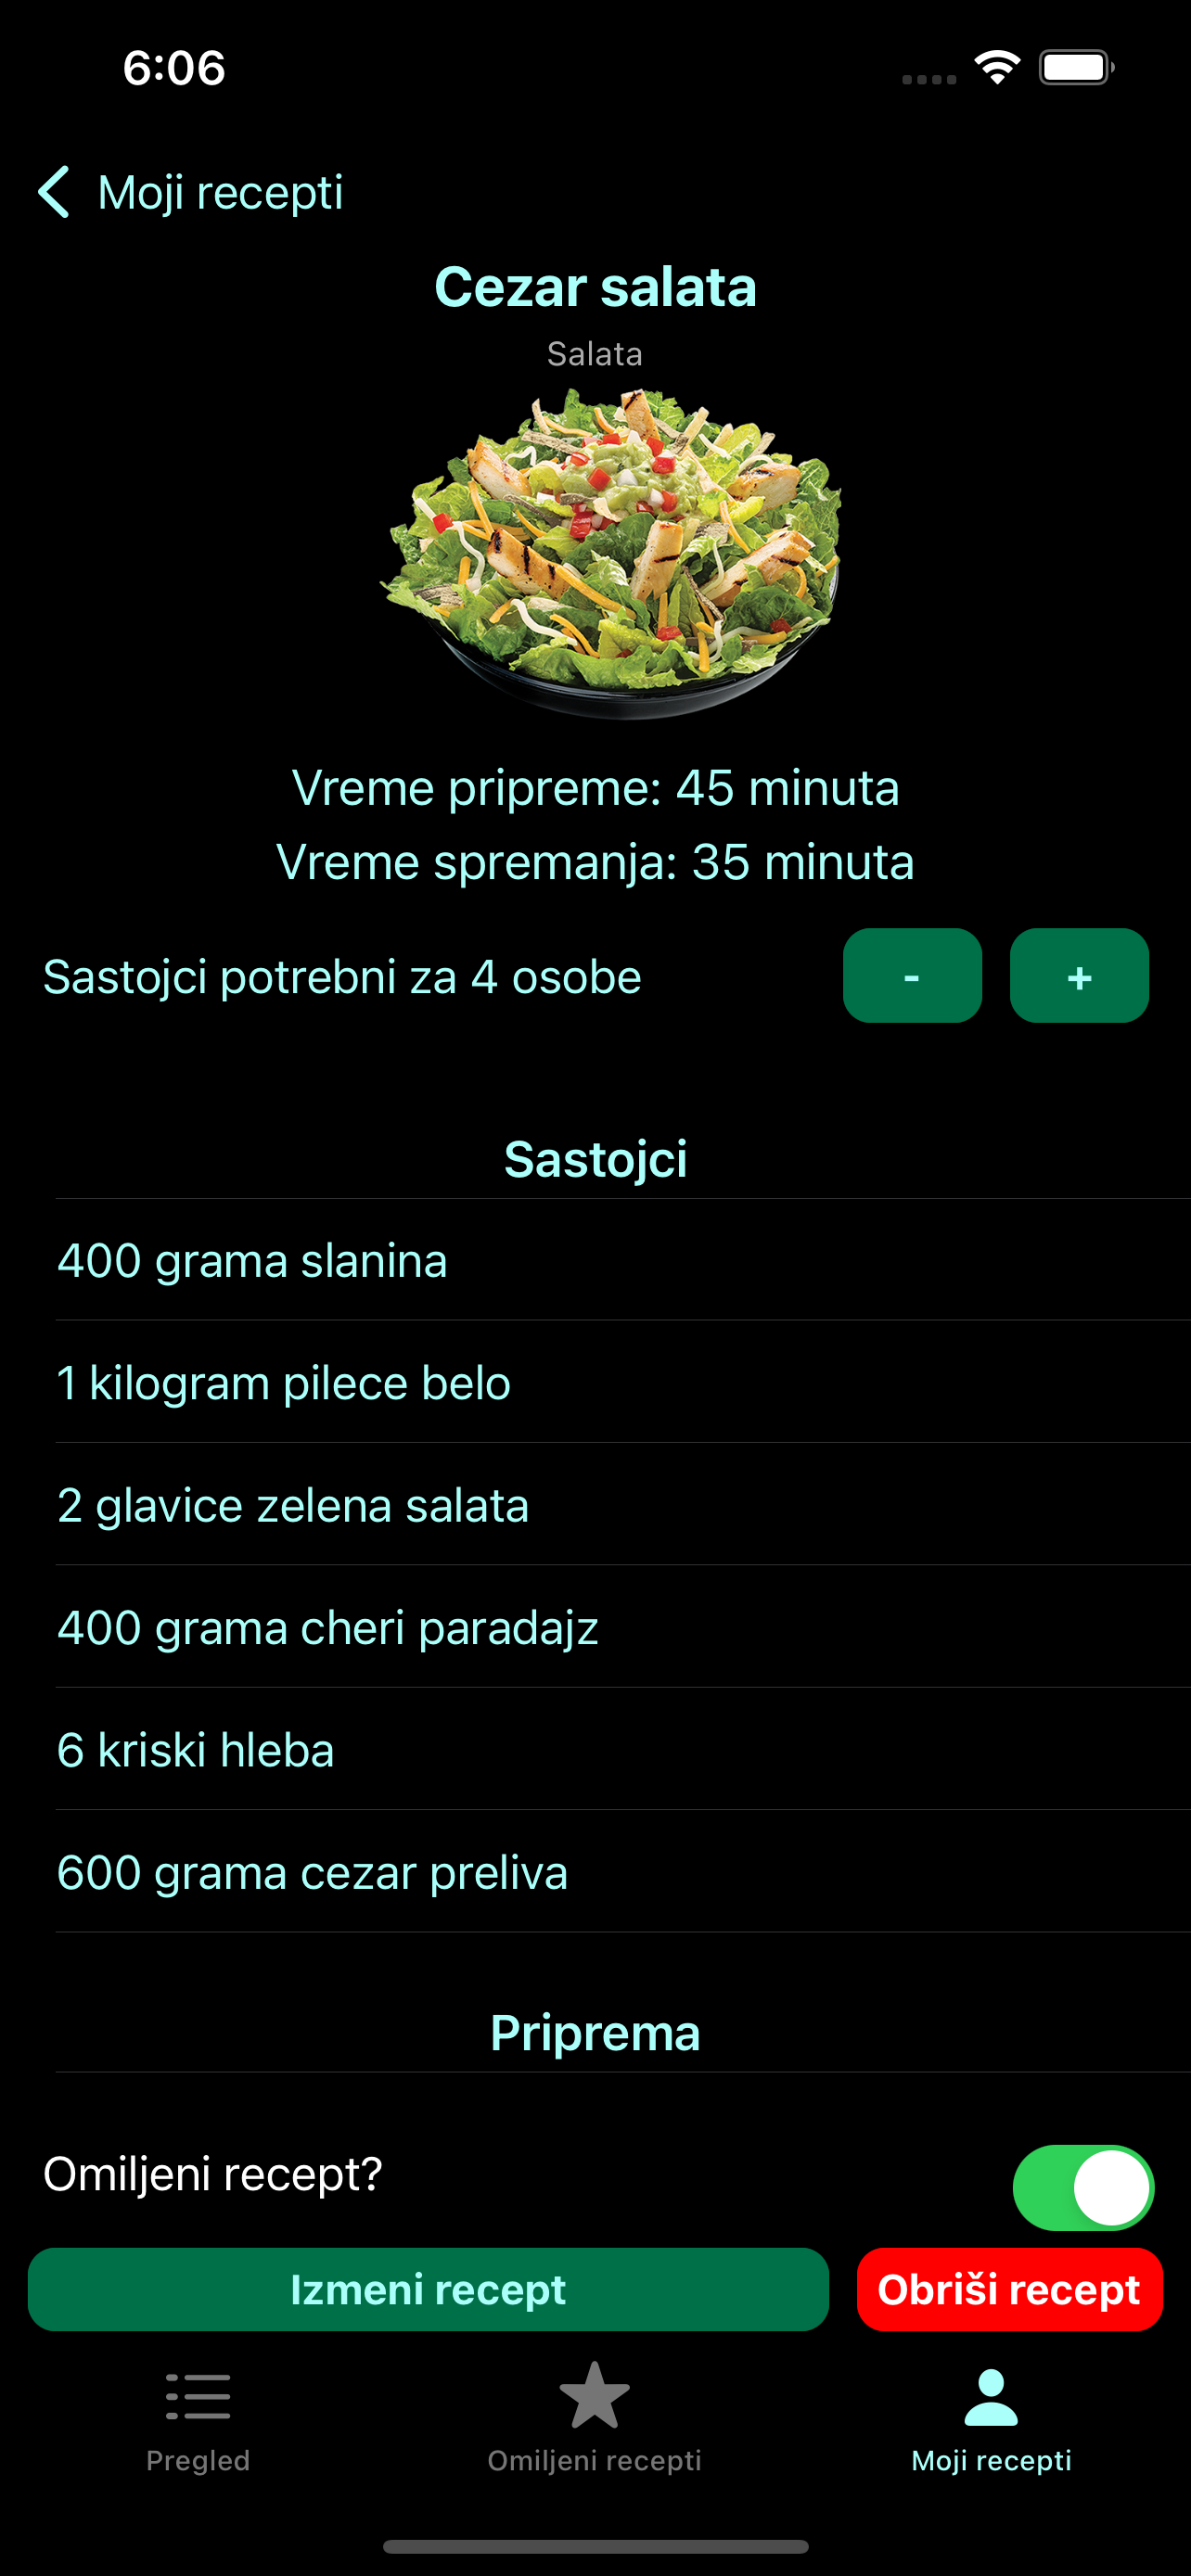
\includegraphics[width=0.475\textwidth]{images/simulators/view images/dark - detail4.png} 
    \hfill
    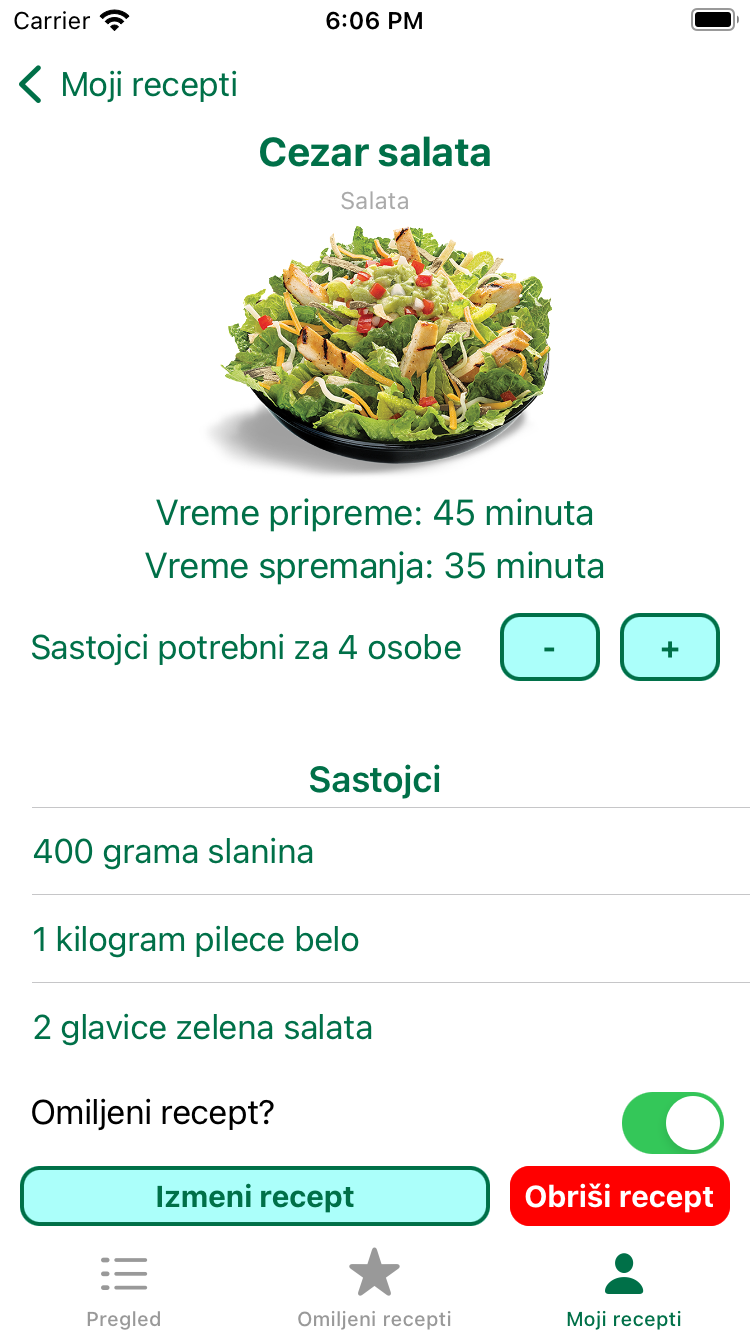
\includegraphics[width=0.475\textwidth]{images/simulators/view images/light - detail4.png} 
    \caption{\textit{Детаљан приказ рецепта --- iPhone 13 (лево) и iPhone SE (десно)}}
    \label{slika:детаљан_рецепт_1}
\end{figure}

\begin{figure} [H]
    \centering
    \captionsetup{justification=centering}
    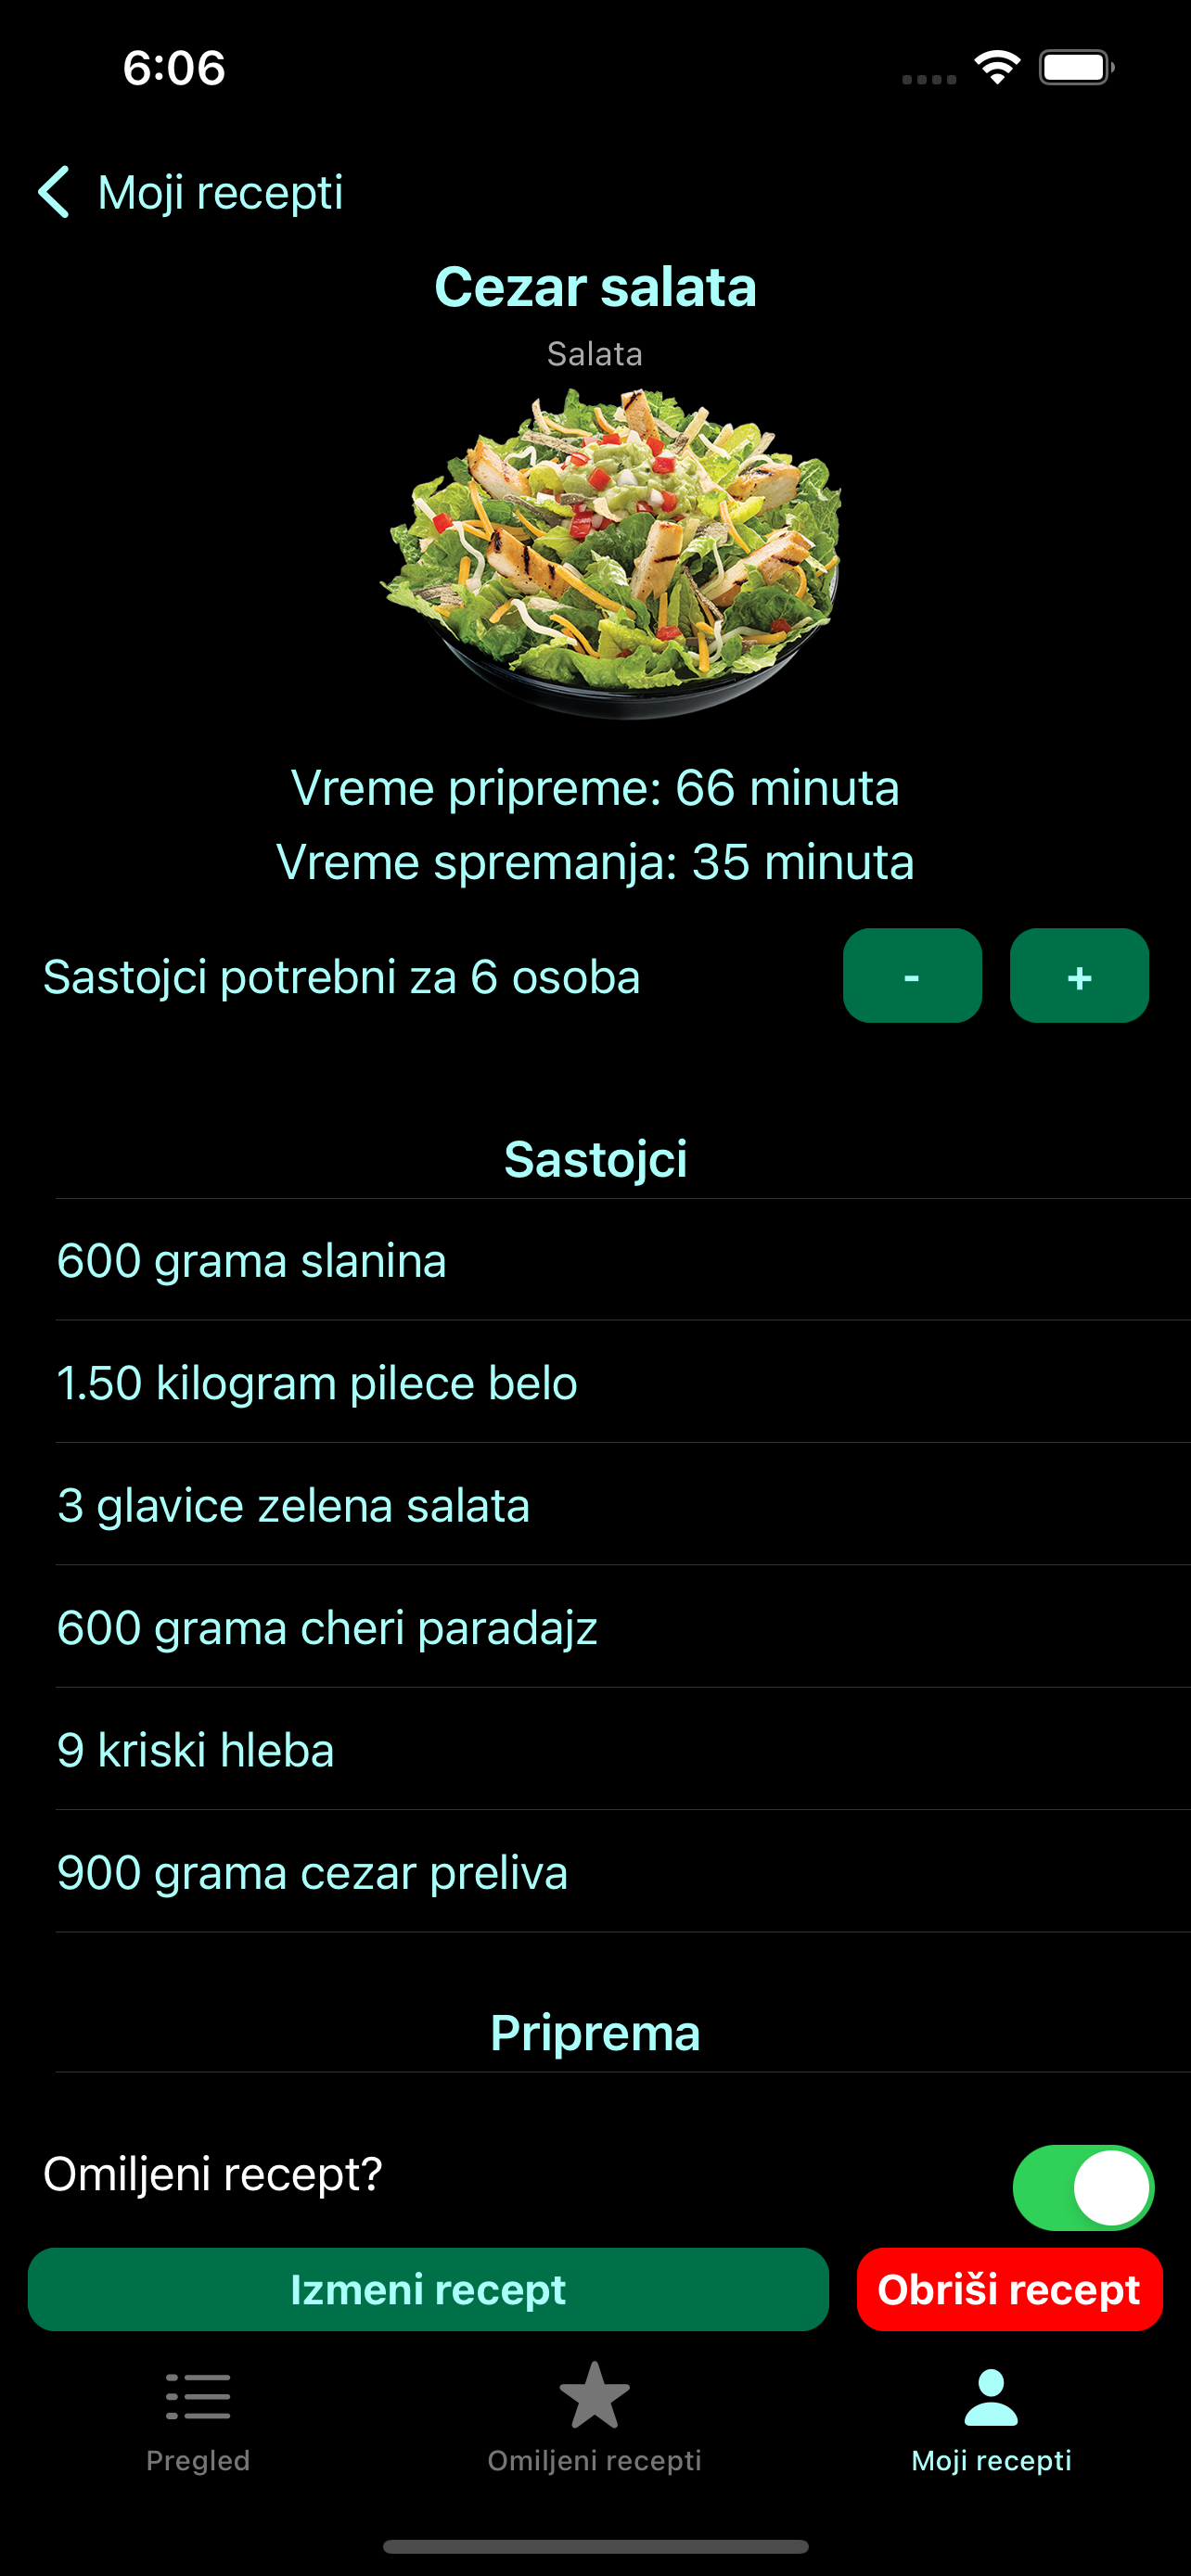
\includegraphics[width=0.475\textwidth]{images/simulators/view images/dark - detail6.png} 
    \hfill
    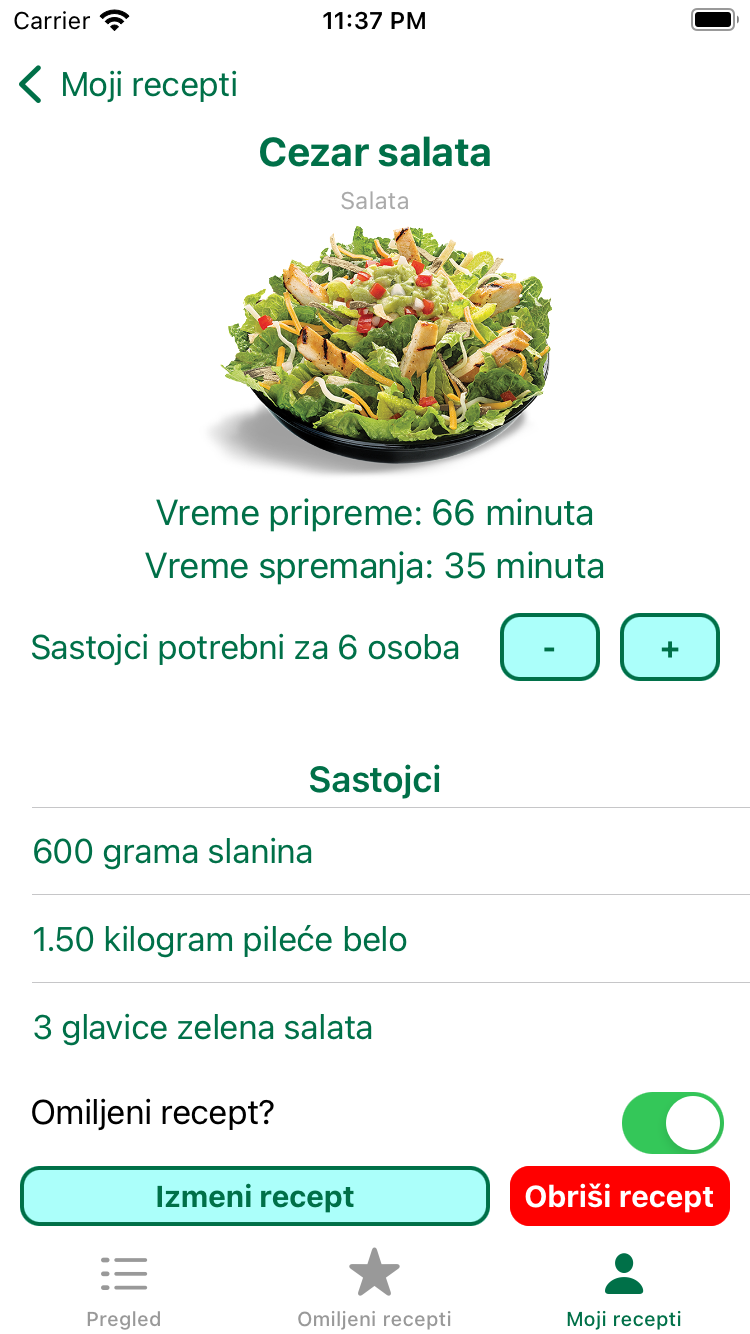
\includegraphics[width=0.475\textwidth]{images/simulators/view images/light - detail6.png} 
    \caption{\textit{Детаљан приказ рецепта за 6 особа --- iPhone 13 (лево) и iPhone SE (десно)}}
    \label{slika:детаљан_рецепт_2_1}
\end{figure}

\subsection{Креирање новог рецепта}
\label{subsec:Креирање новог рецепта}

\indent Приликом креирања новог рецепта од корисника се тражи да унесе све потребне информације које су наведене у претходном поглављу. Изглед погледа додавања новог рецепта може се видети на слици \ref{slika:нов_рецепт_1}.

\begin{figure} [H]
    \centering
    \captionsetup{justification=centering}
    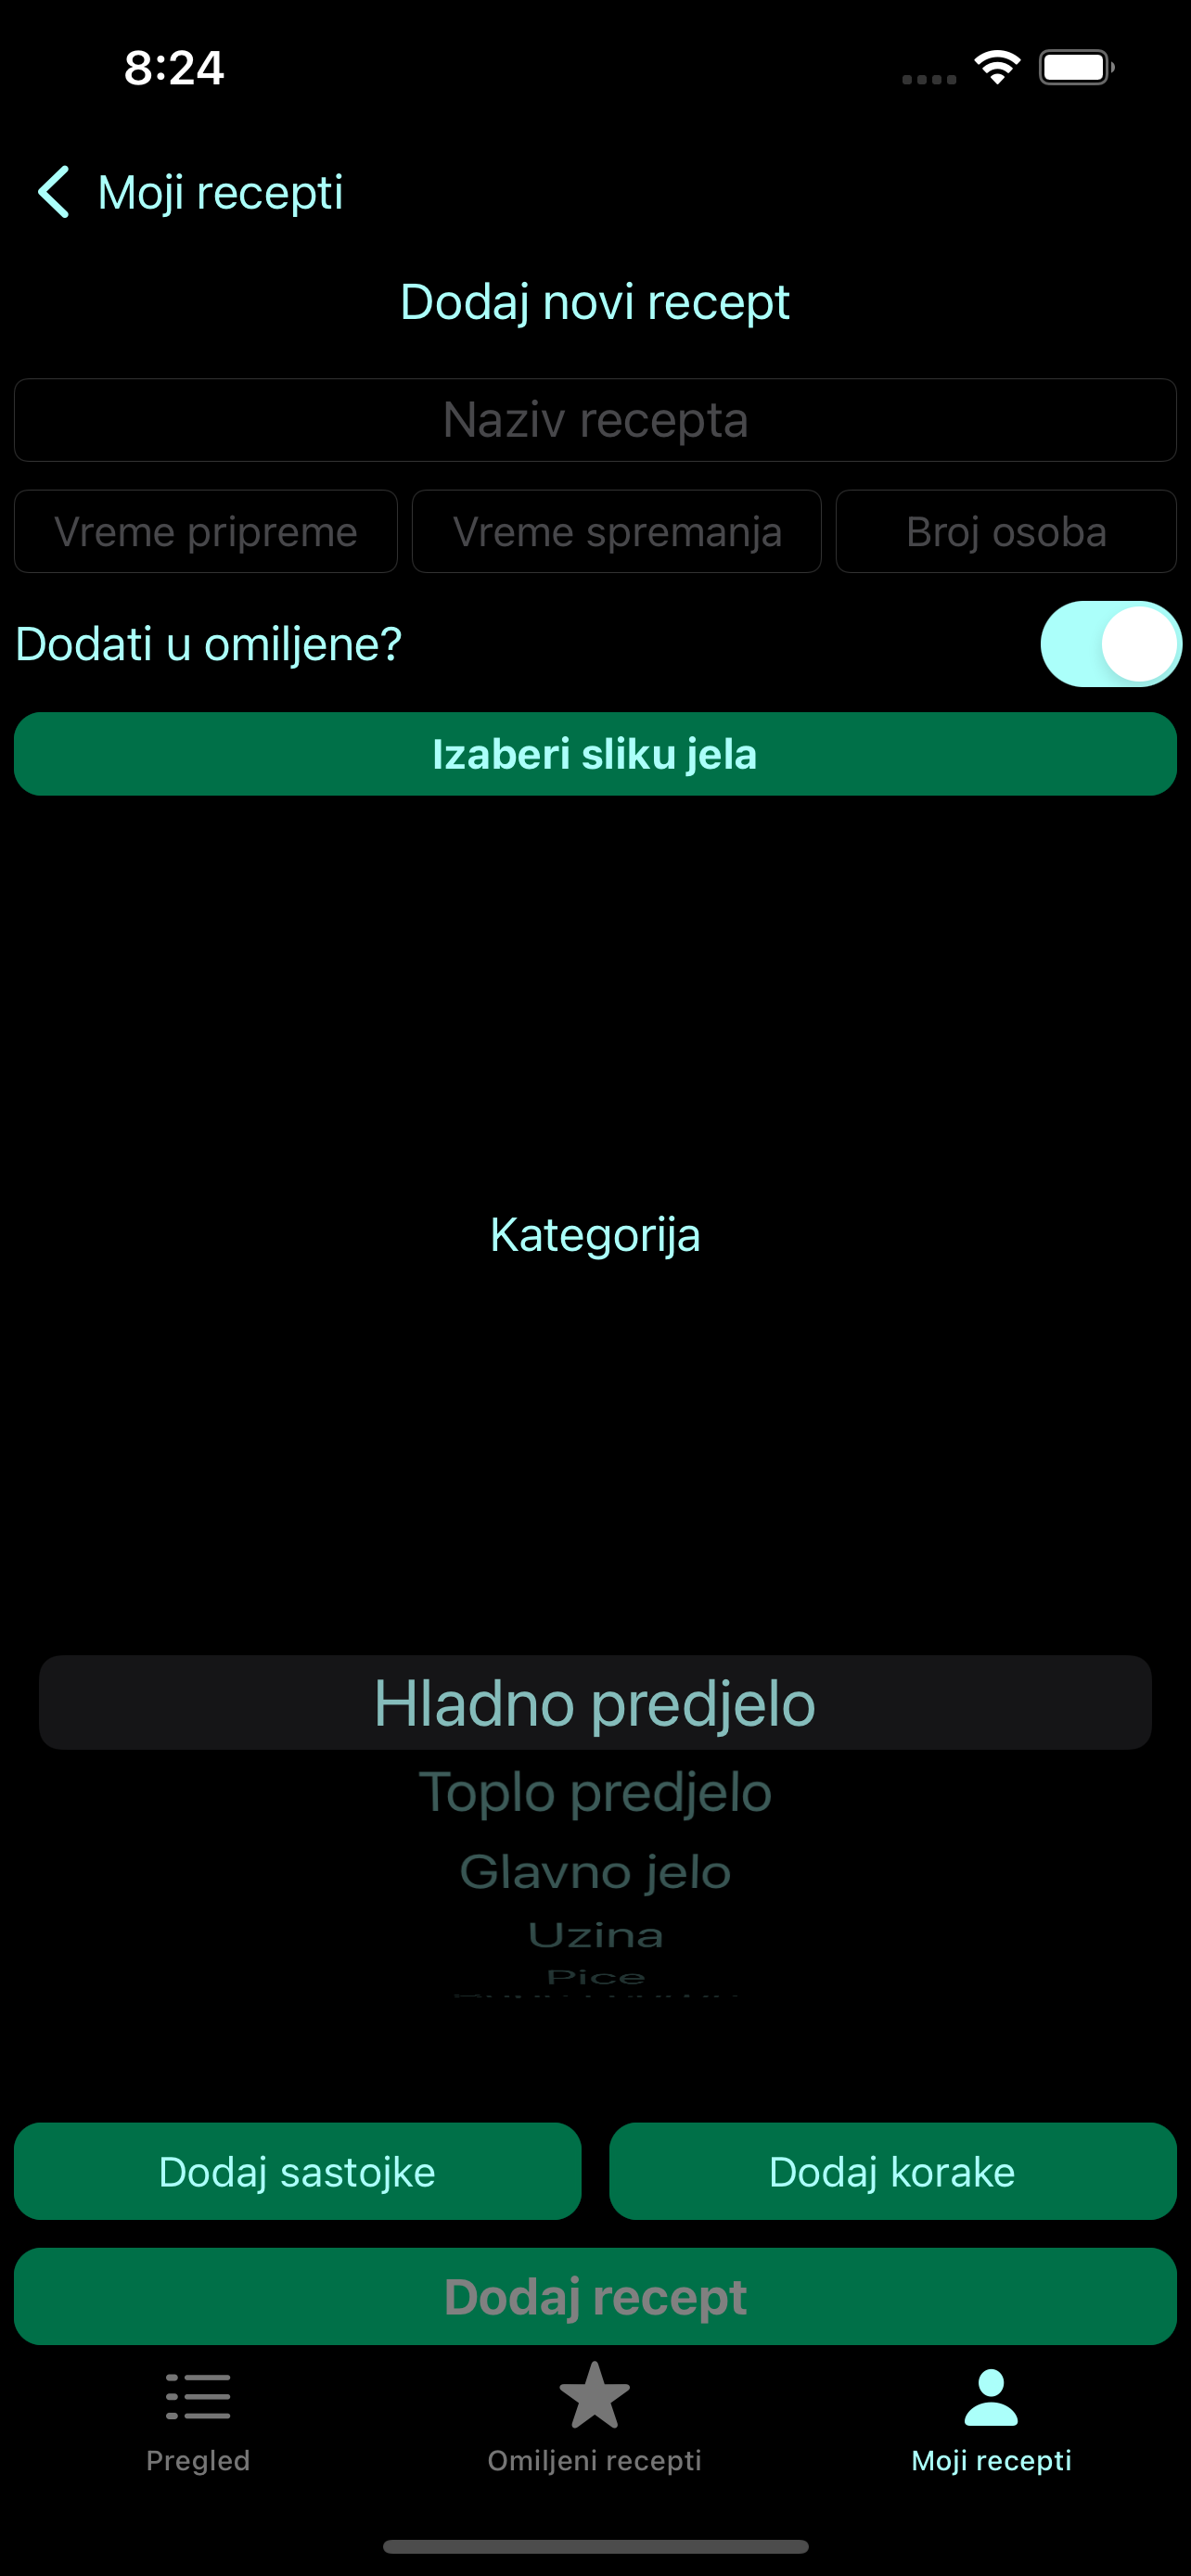
\includegraphics[width=0.475\textwidth]{images/simulators/view images/dark - new.png} 
    \hfill
    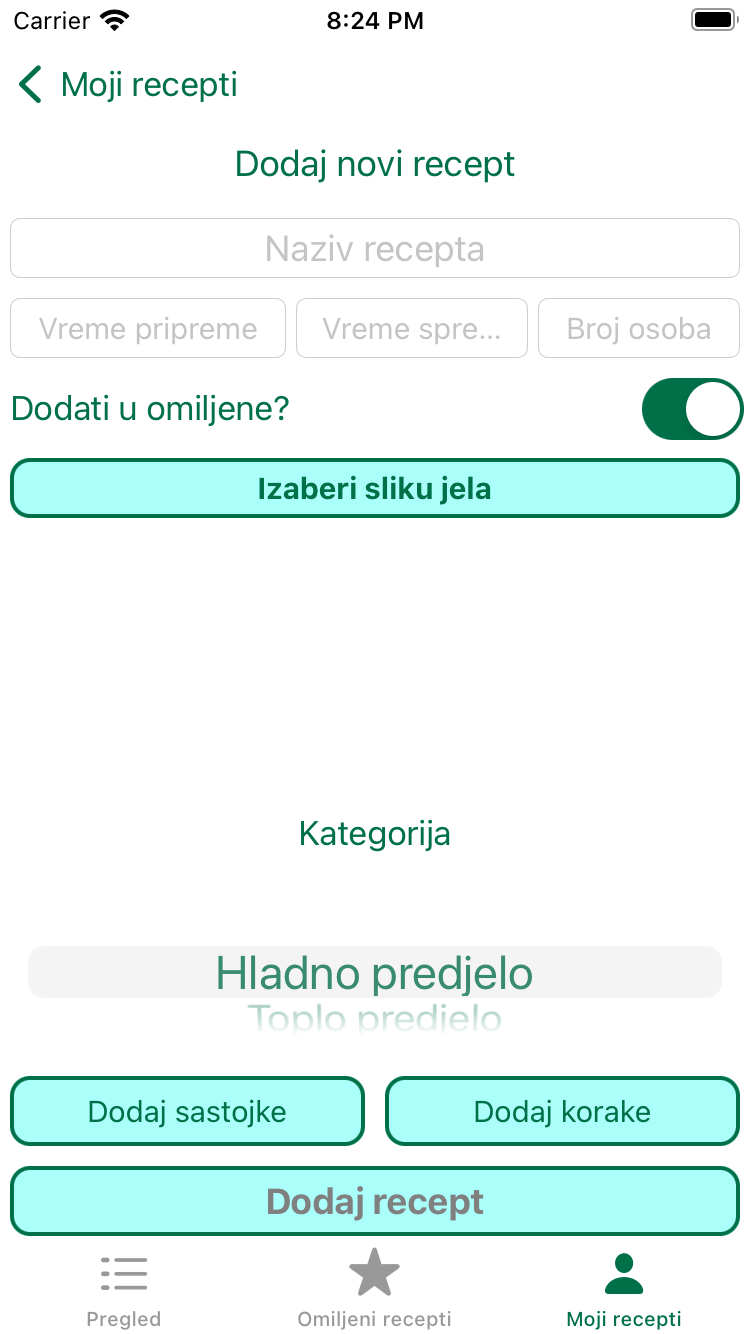
\includegraphics[width=0.475\textwidth]{images/simulators/view images/light - new.png} 
    \caption{\textit{Нов рецепт --- iPhone 13 (лево) и iPhone SE (десно)}}
    \label{slika:нов_рецепт_1}
\end{figure}

\subsection{Измена и брисање постојећег рецепта}
\label{subsec:Измена и брисање постојећег рецепта}

\indent Корисник има могућност промене свих рецепата које је додао. Приказ изгледа погледа измене рецепта налази се на слици \ref{slika:измена_рецепта_1}. Постоји могућност измене, брисања и додавања нових састојака (слика \ref{slika:измена_састојака_2_1}), измене, брисања и додавања нових корака припреме (слика \ref{slika:измена_корака_2_1}).

\begin{figure} [H]
    \centering
    \captionsetup{justification=centering}
    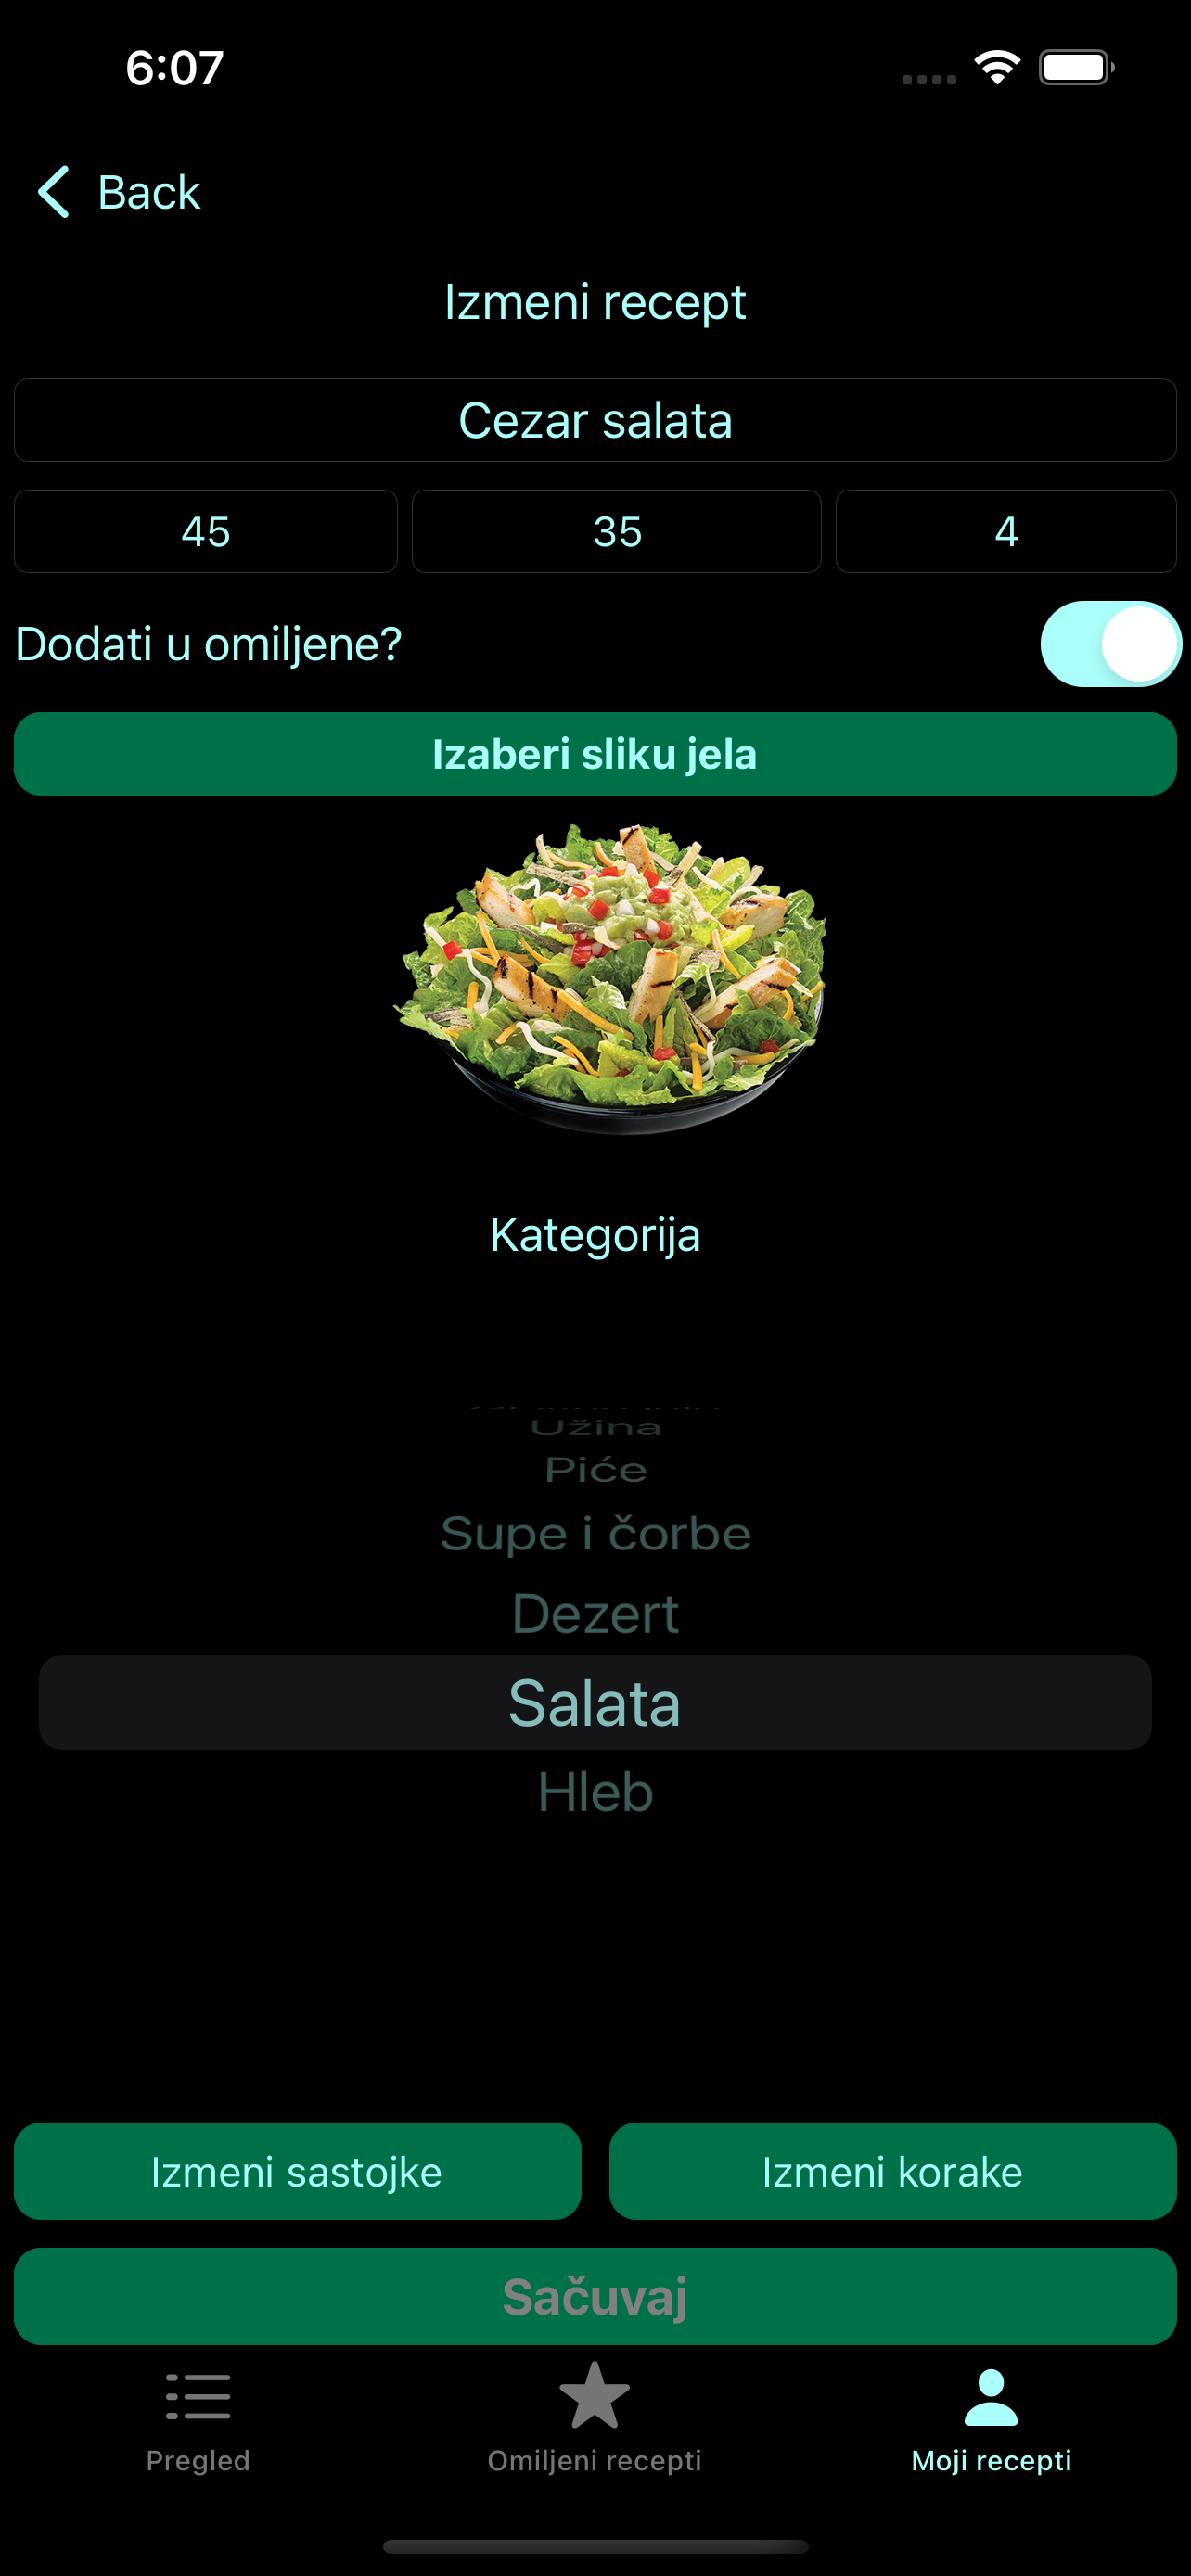
\includegraphics[width=0.475\textwidth]{images/simulators/view images/dark - change.png} 
    \hfill
    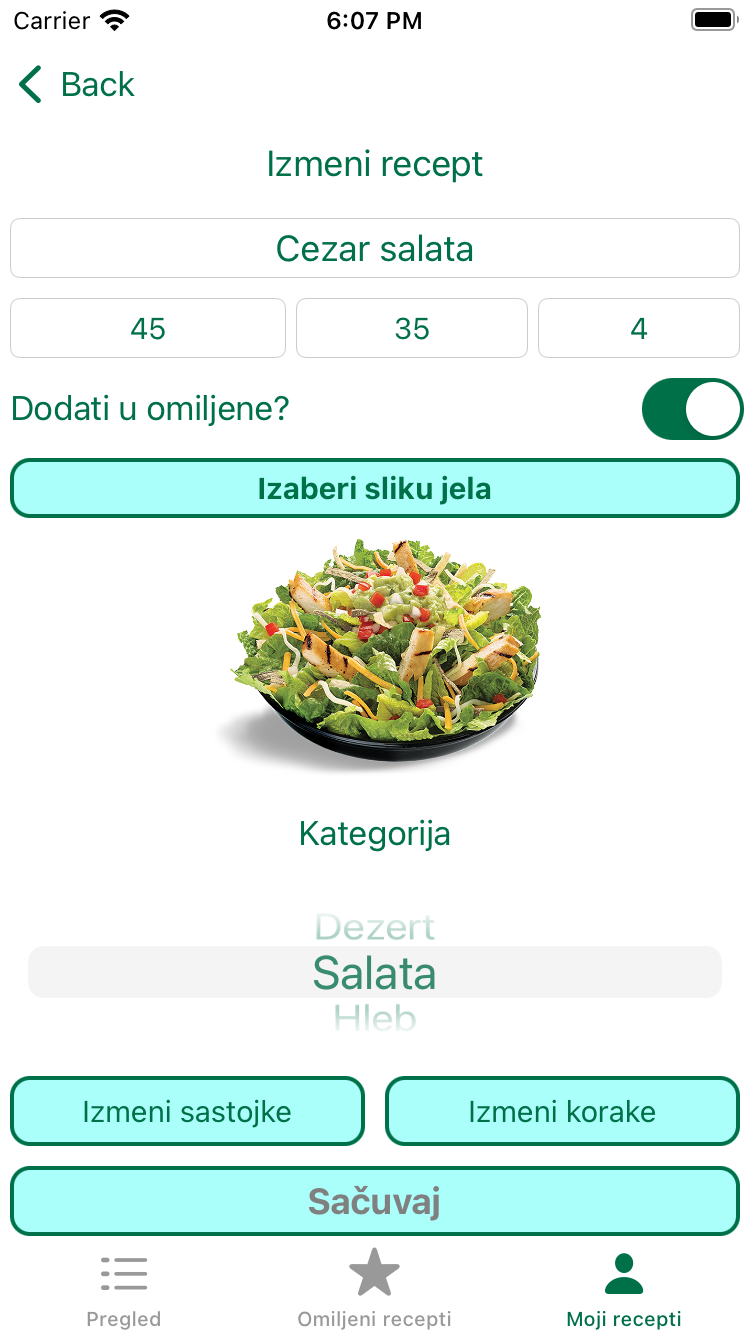
\includegraphics[width=0.475\textwidth]{images/simulators/view images/light - change.png} 
    \caption{\textit{Измена рецепта --- iPhone 13 (лево) и iPhone SE (десно)}}
    \label{slika:измена_рецепта_1}
\end{figure}

\begin{figure} [H]
    \centering
    \captionsetup{justification=centering}
    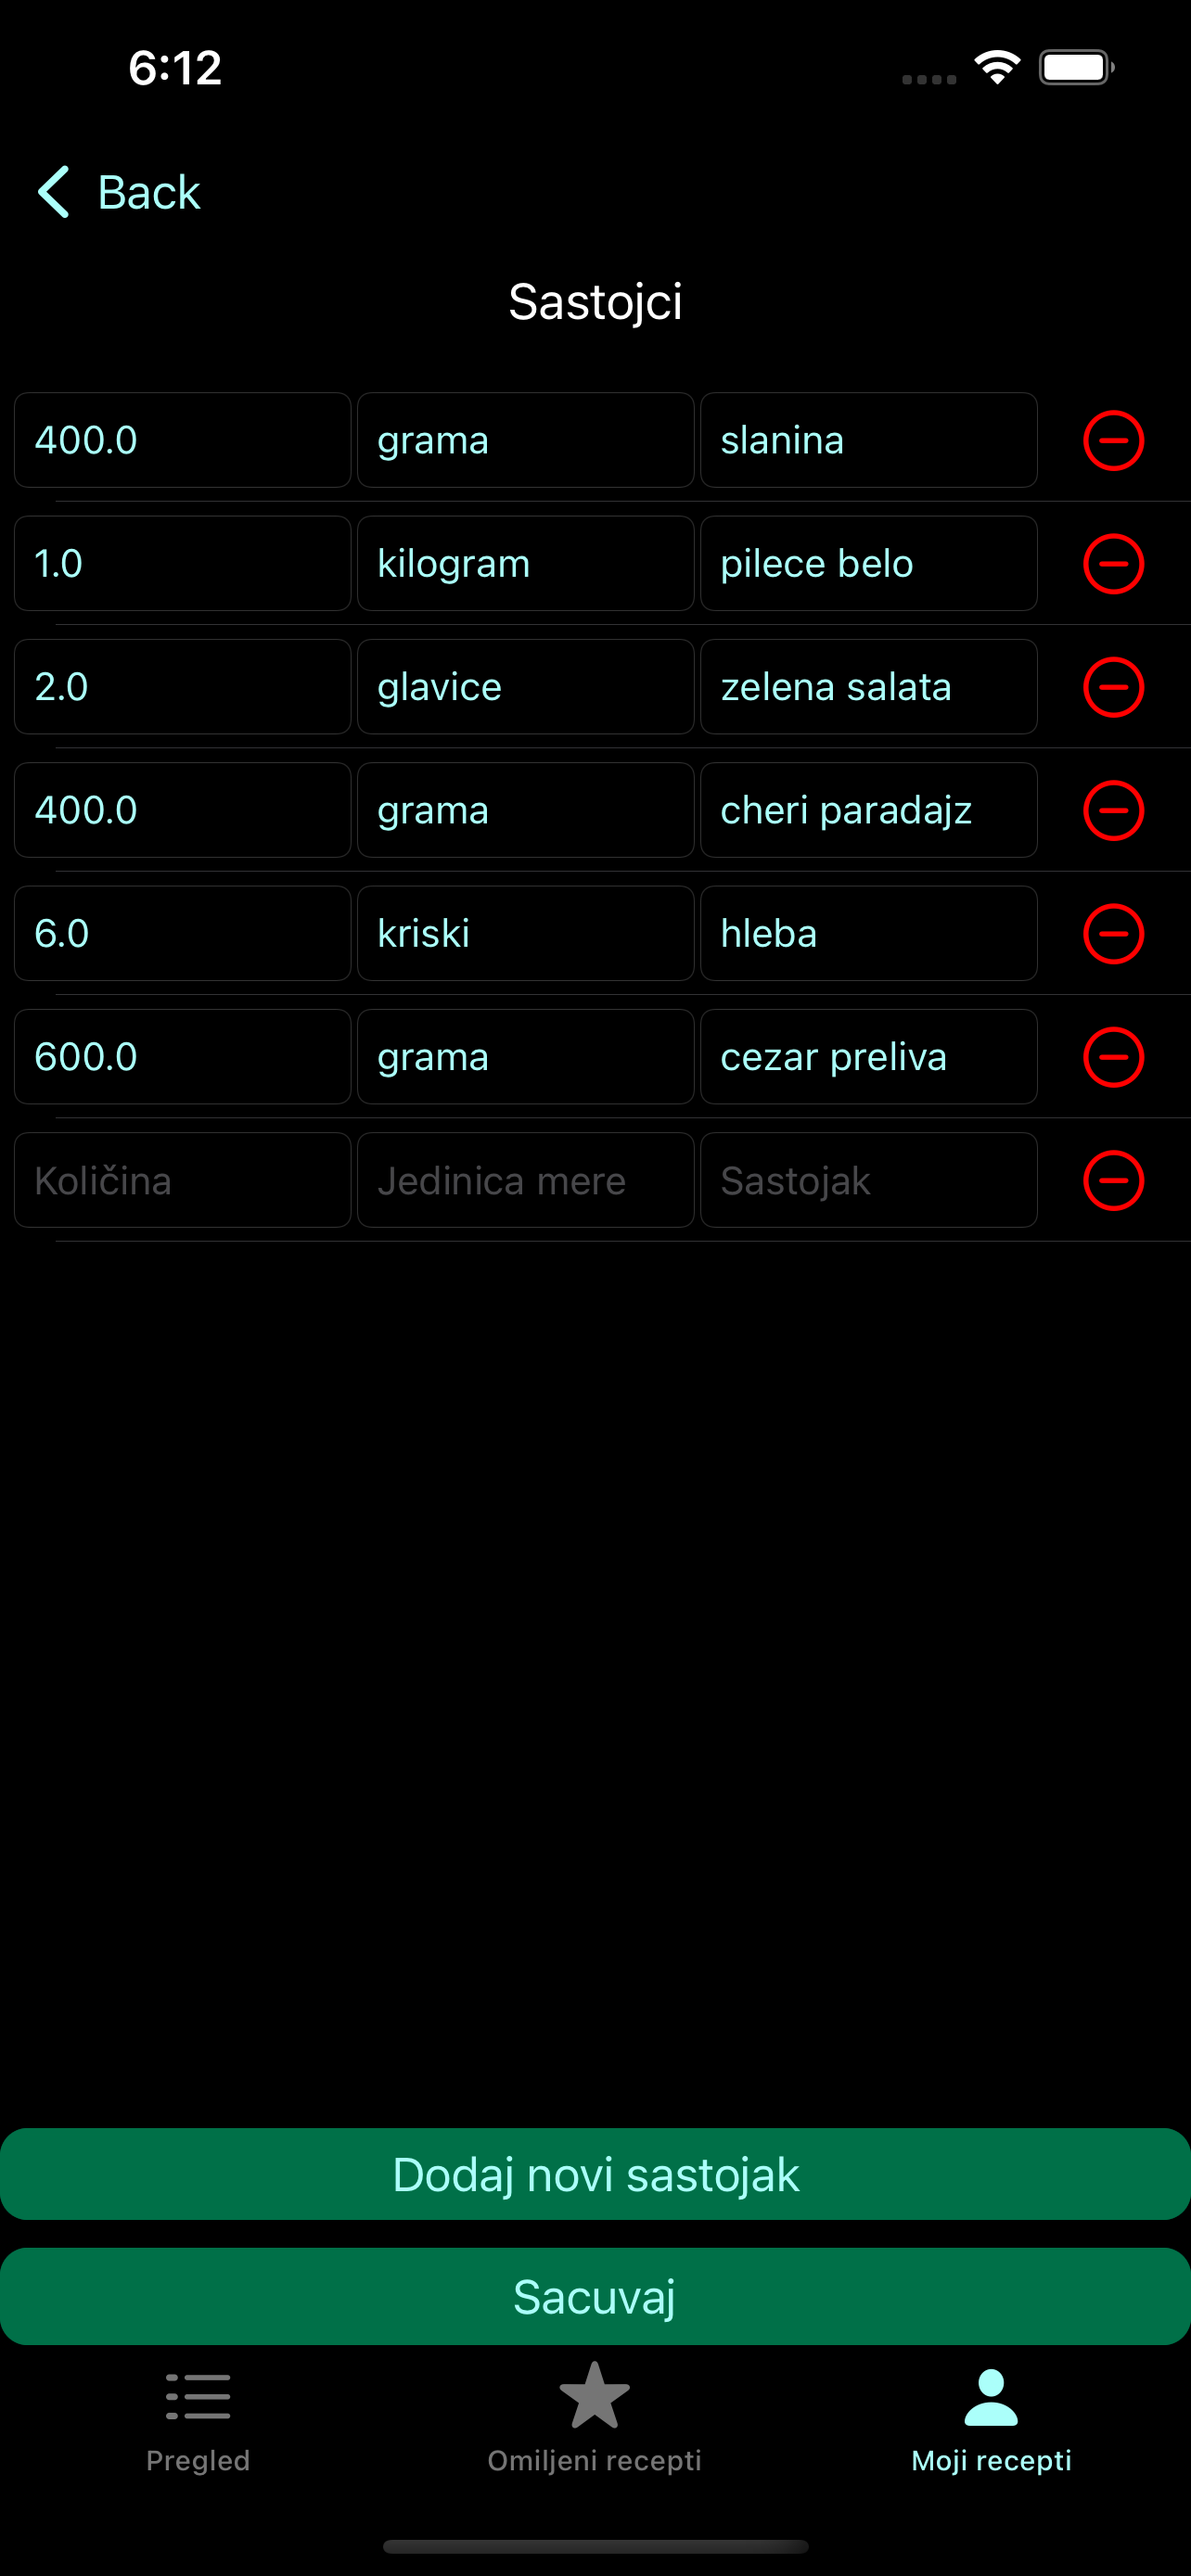
\includegraphics[width=0.475\textwidth]{images/simulators/view images/dark - ingredients2.png}
    \hfill
    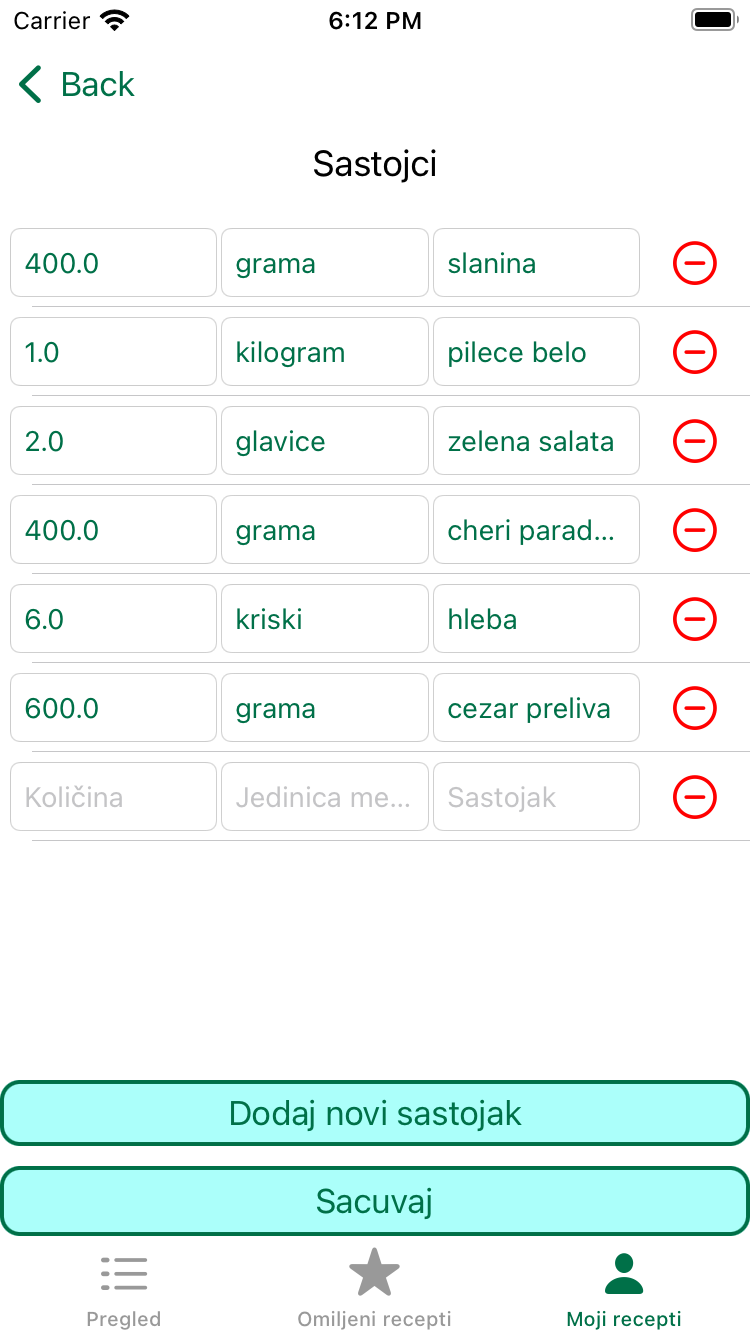
\includegraphics[width=0.475\textwidth]{images/simulators/view images/light - ingredients2.png}
    \caption{\textit{Измена тренутних састојака за припрему рецепта уз додавање новог састојка --- iPhone 13 (лево) и iPhone SE (десно)}}
    \label{slika:измена_састојака_2_1}
\end{figure}

\begin{figure} [H]
    \centering
    \captionsetup{justification=centering}
    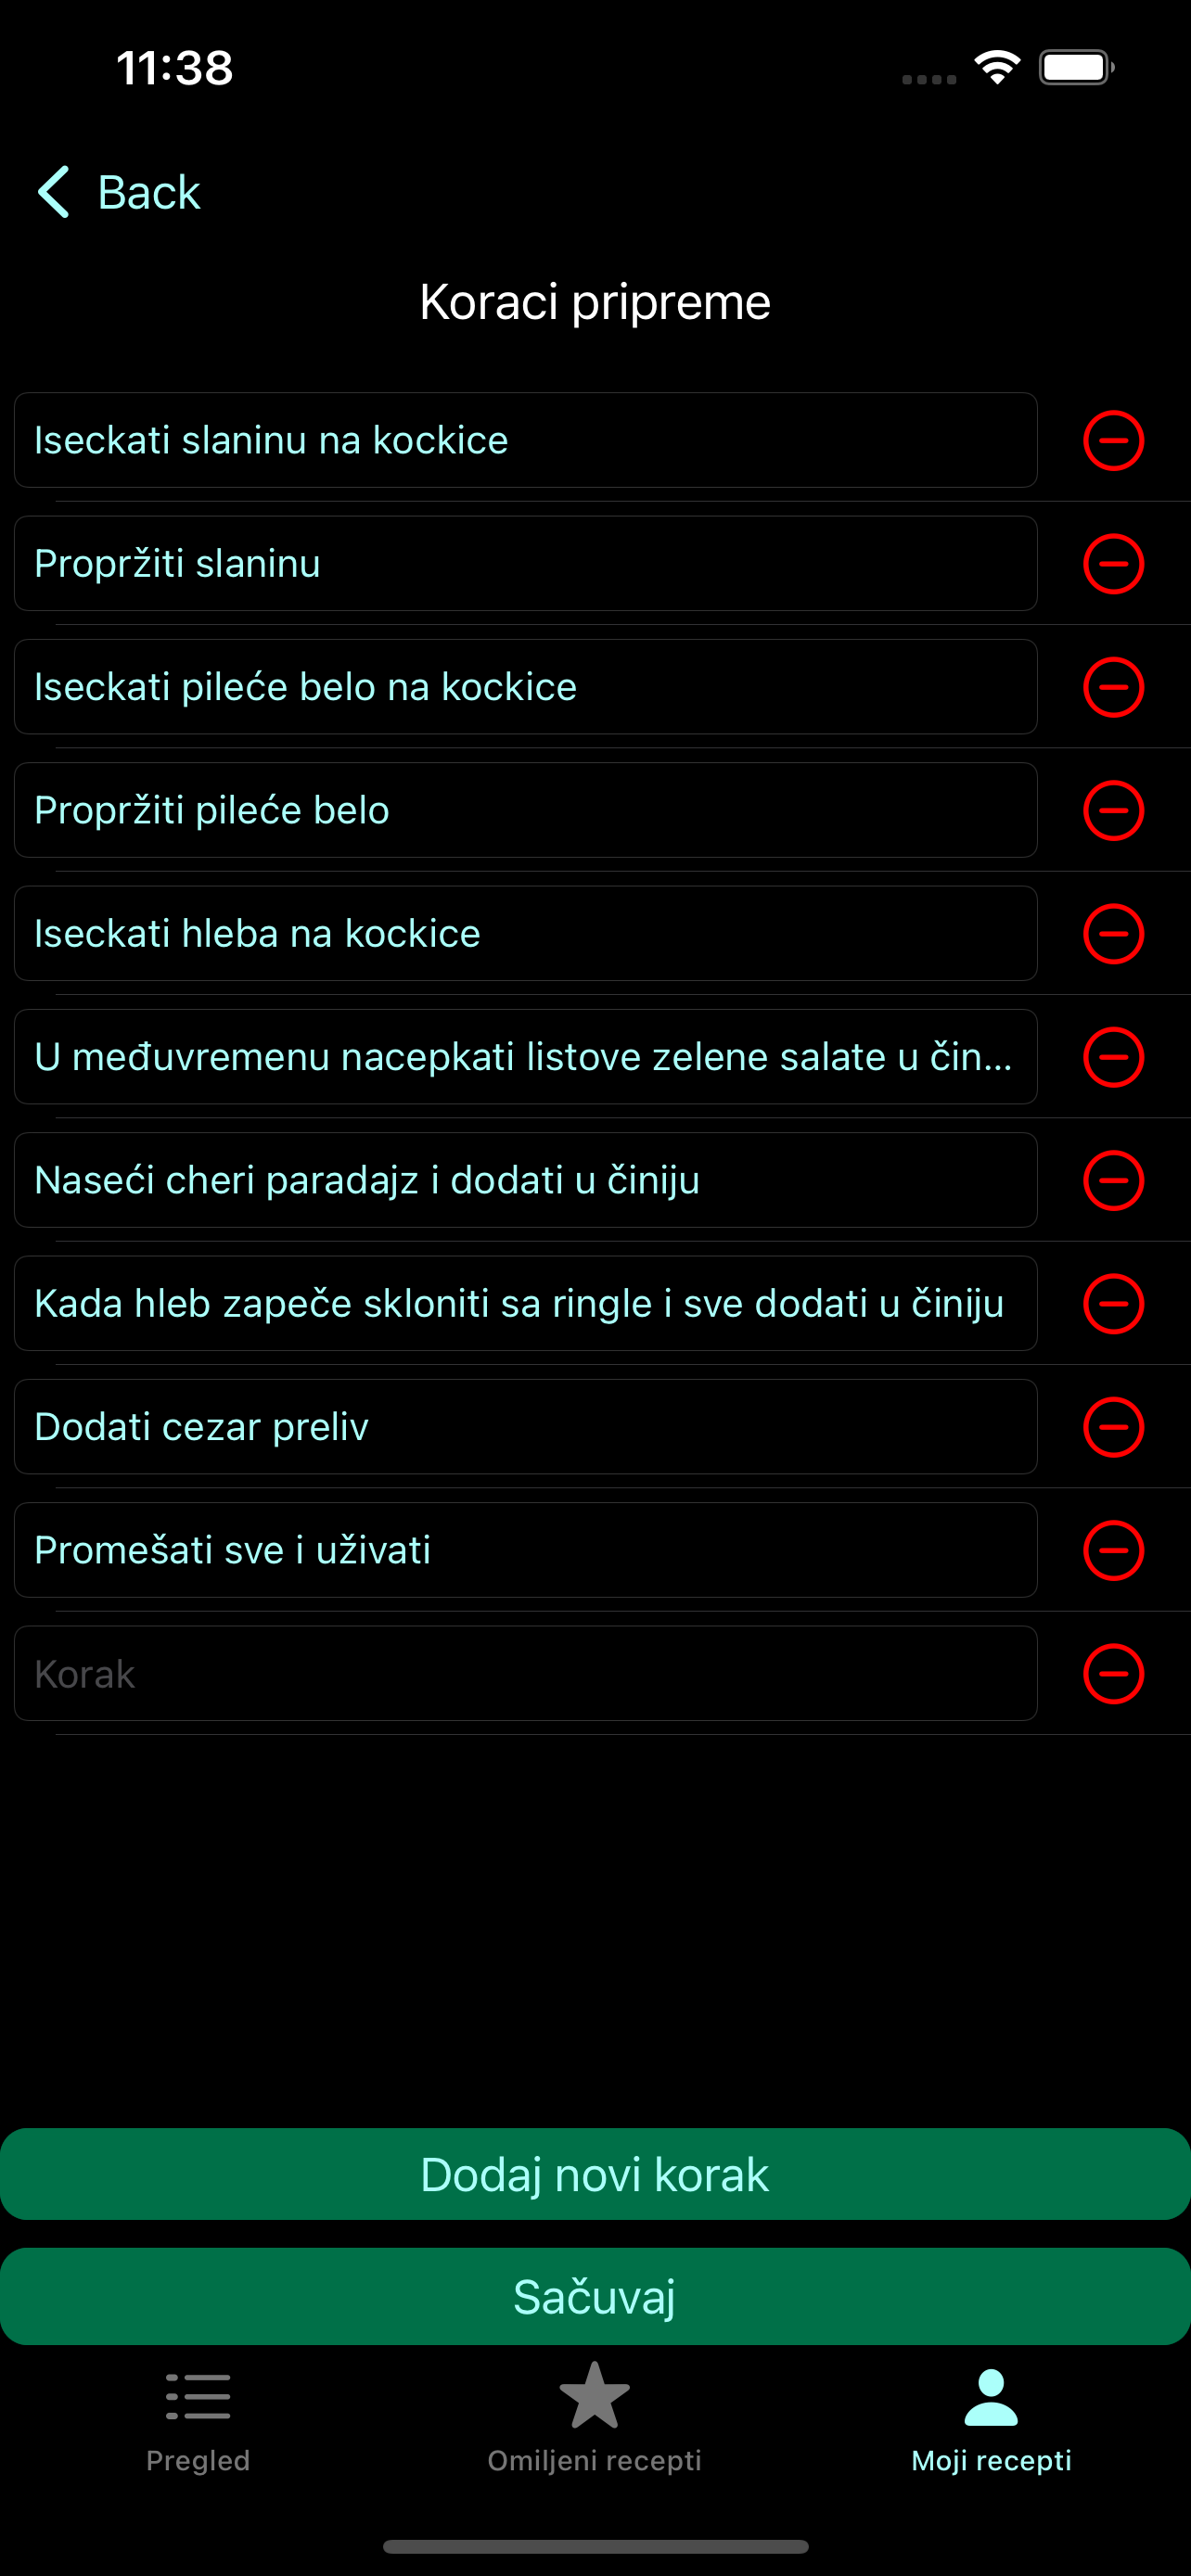
\includegraphics[width=0.475\textwidth]{images/simulators/view images/dark - steps2.png} 
    \hfill
    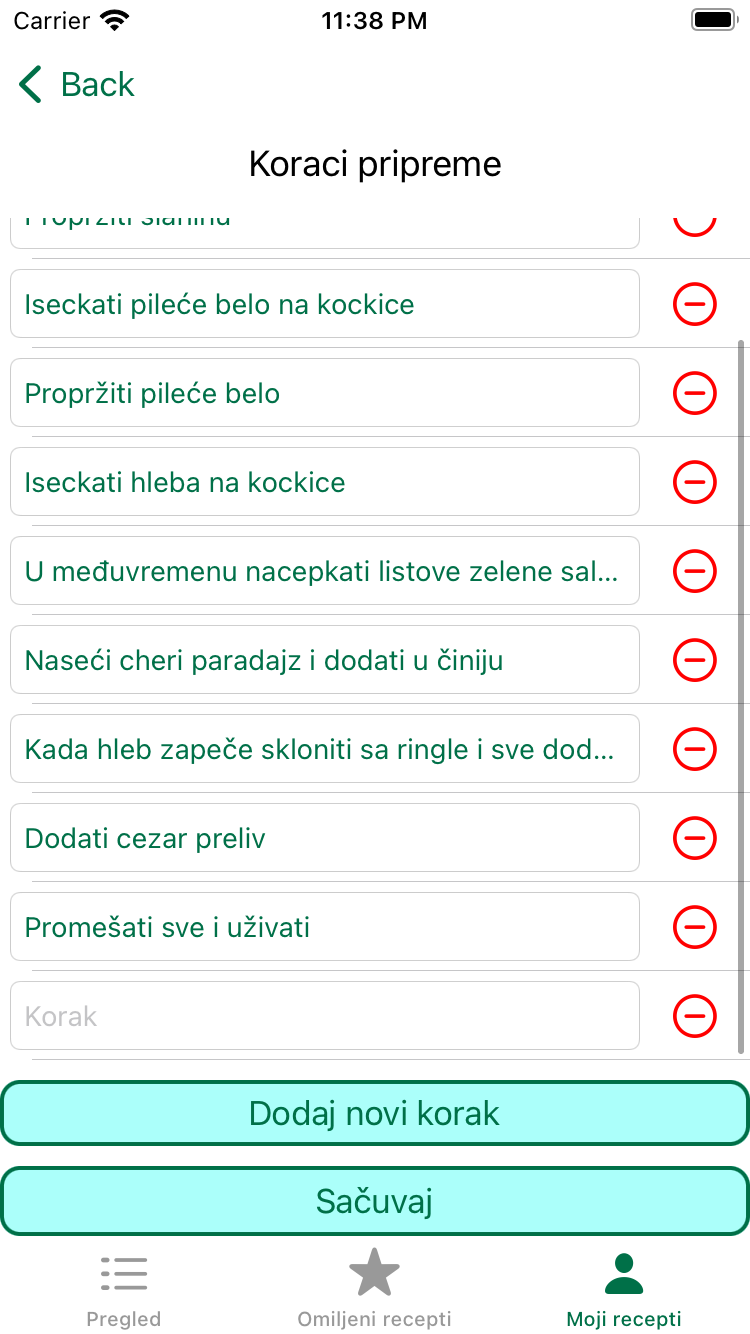
\includegraphics[width=0.475\textwidth]{images/simulators/view images/light - steps2.png} 
    \caption{\textit{Измена тренутних корака за припрему рецепта уз додавање новог корака припреме --- iPhone 13 (лево) и iPhone SE (десно)}}
    \label{slika:измена_корака_2_1}
\end{figure}

\indent Уколико корисник жели, може и обрисати рецепте које је додао кликом на дугме "Обриши рецепт" унутар детаљног приказа рецепта, након чега ће му бити приказано упозорење у којем ће моћи да потврди брисање рецепта или да од њега одустане. Приказ упозорења приликом брисања рецепта налази се на слици \ref{slika:брисање_рецепта_1}.

\begin{figure} [H]
    \centering
    \captionsetup{justification=centering}
    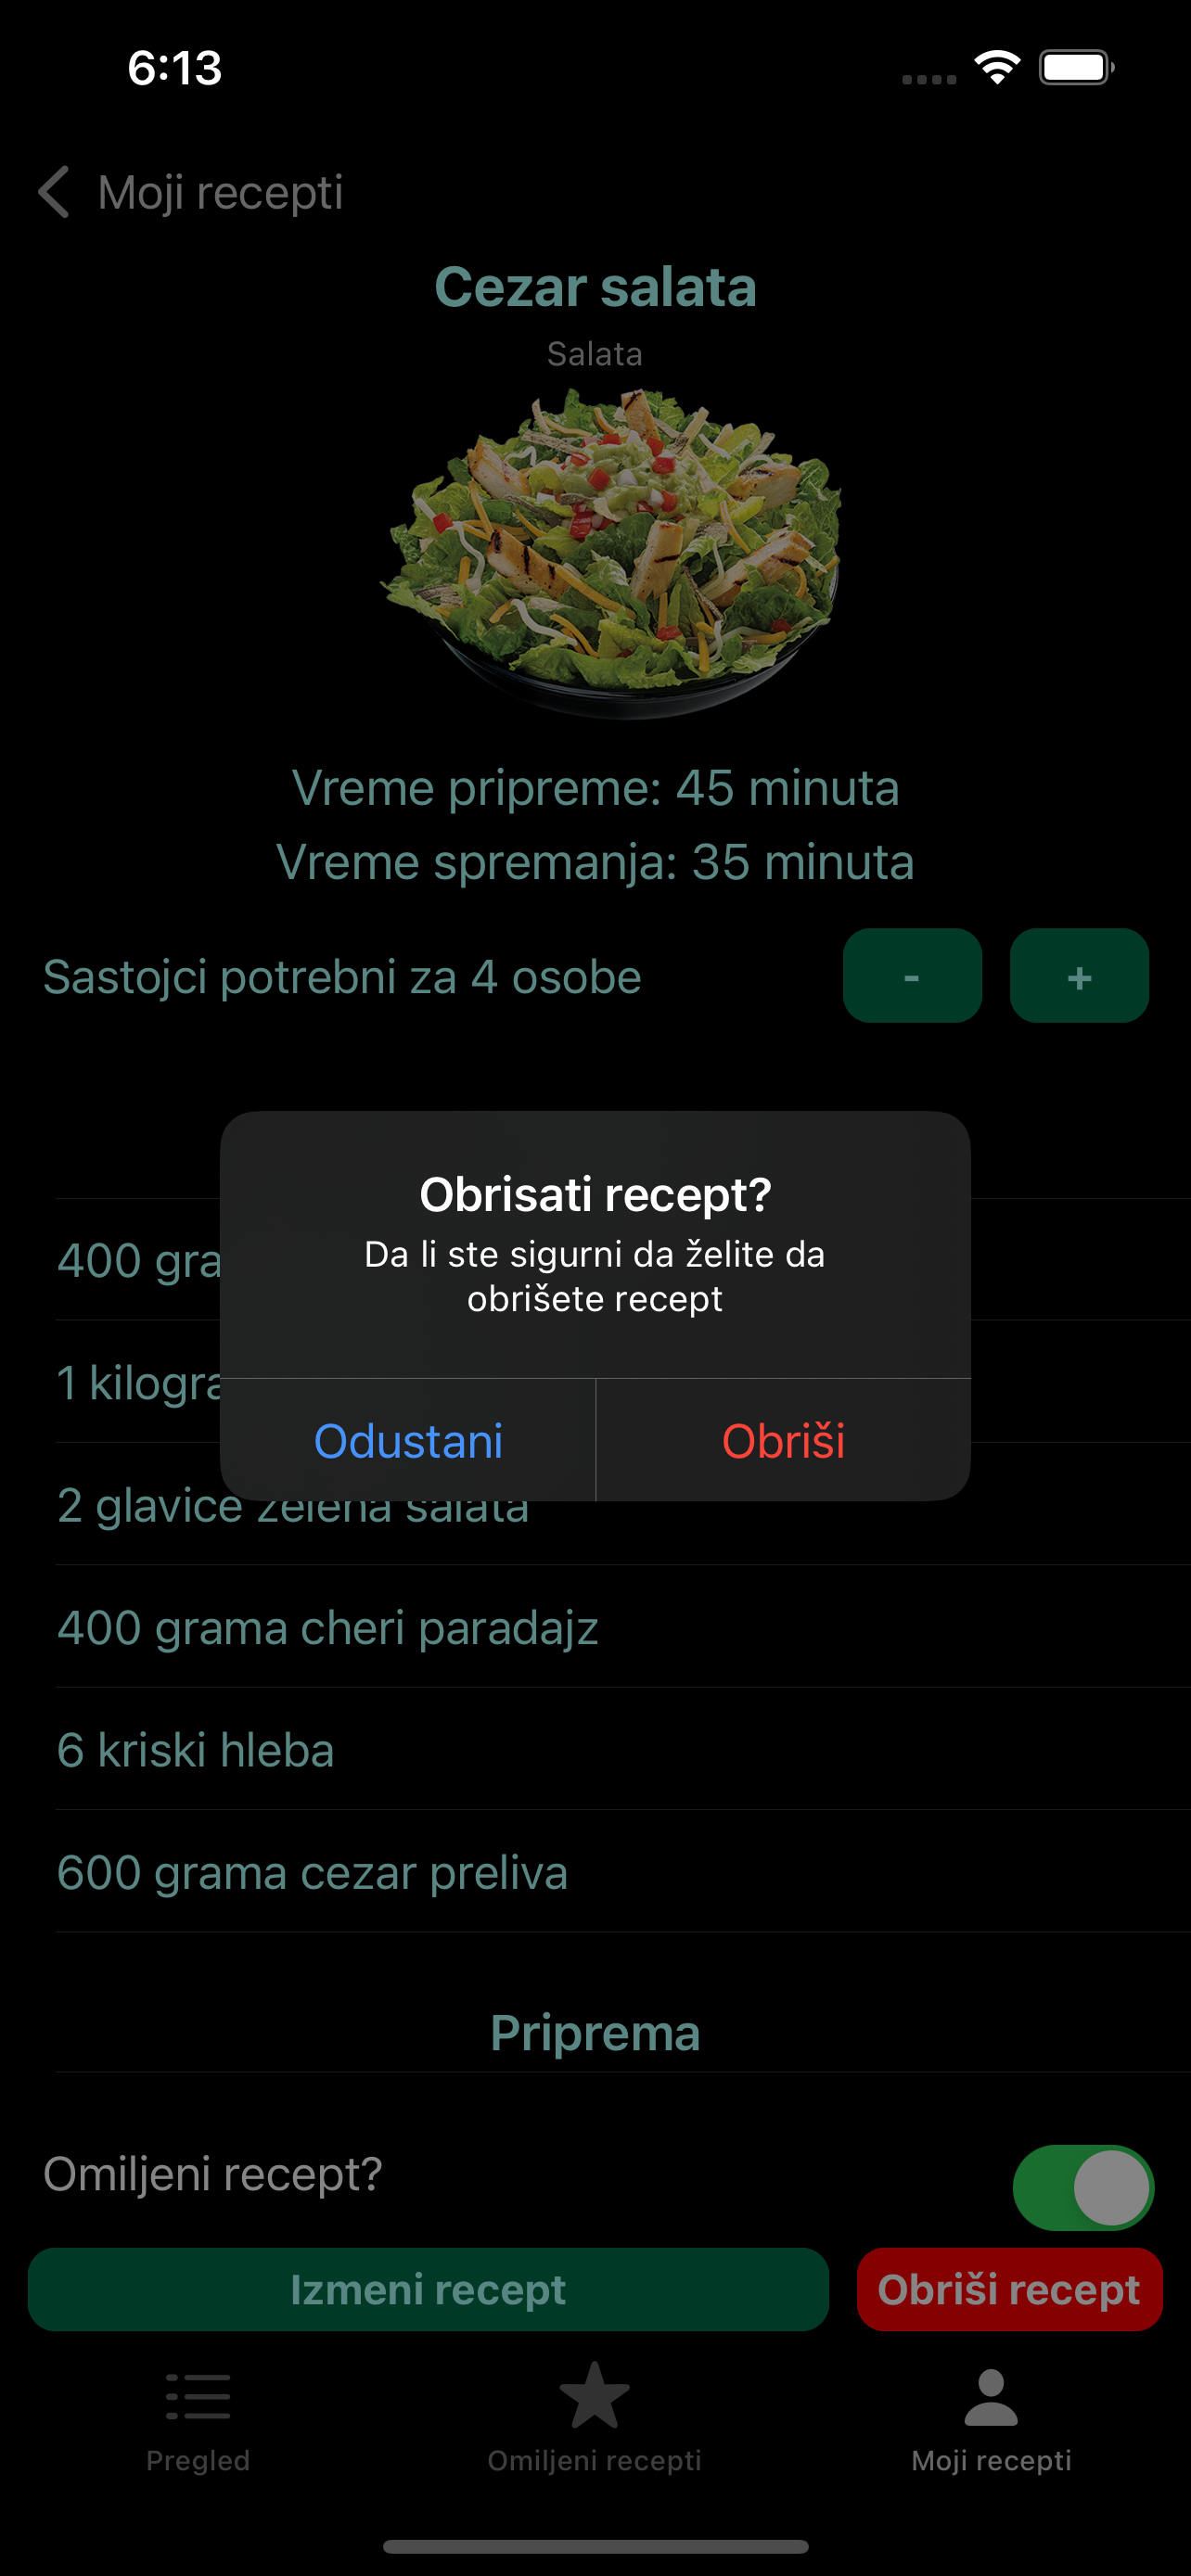
\includegraphics[width=0.475\textwidth]{images/simulators/view images/dark - delete.png} 
    \hfill
    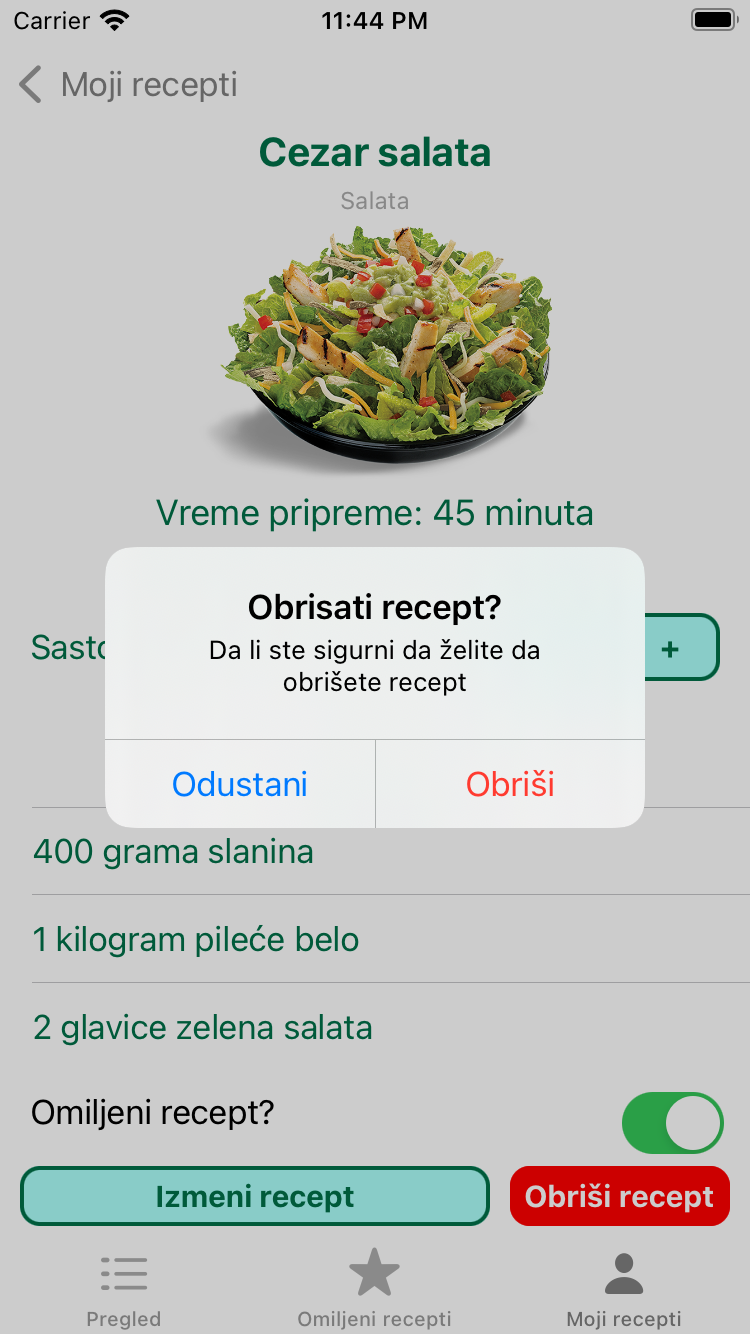
\includegraphics[width=0.475\textwidth]{images/simulators/view images/light - delete.png}
    \caption{\textit{Брисање рецепта --- iPhone 13 (лево) и iPhone SE (десно)}}
    \label{slika:брисање_рецепта_1} 
\end{figure}

\subsection{Приказ виџета} 

\indent Корисник може додати виџет на почетни екран из виџет галерије, где се налазе оба типа виџета ове апликације (први тип у све три величине, док је други доступан само у великој величини) који ће детаљније бити објашњени у наставку. Приказ додавања виџета из галерије представљен је на слици \ref{slika:додавање_виџета_1}.

\begin{figure} [H]
    \centering
    \captionsetup{justification=centering}
    
\includegraphics[width=0.475\textwidth]{images/simulators/view images/dark - add widget.png} 
    \hfill
    
\includegraphics[width=0.475\textwidth]{images/simulators/view images/light - add widget.png} 
    \caption{\textit{Додавање виџета --- iPhone 13 (лево) и iPhone SE (десно)}}
    \label{slika:додавање_виџета_1}
\end{figure}

\indent Први тип виџета (назван "Рецепт на клик") доступан је корисницима у све три величине (мала, средња и велика). Мали виџет приказује слику рецепта уз његов назив и може послужити као подсетник кориснику шта је испланирао да спрема или као пречица ка детаљном опису тог рецепта. Средњи виџет је проширење малог виџета који додатно приказује састојке или кораке припреме рецепта, параметар који је конфигурабилан од стране корисника. Приказ малог и средњег виџета може се видети на слици \ref{slika:приказ_виџета_1_1}.

\begin{figure} [H]
    \centering
    \captionsetup{justification=centering}
    \includegraphics[width=0.475\textwidth]{images/simulators/view images/dark - widgets 1-1.png}
    \hfill
    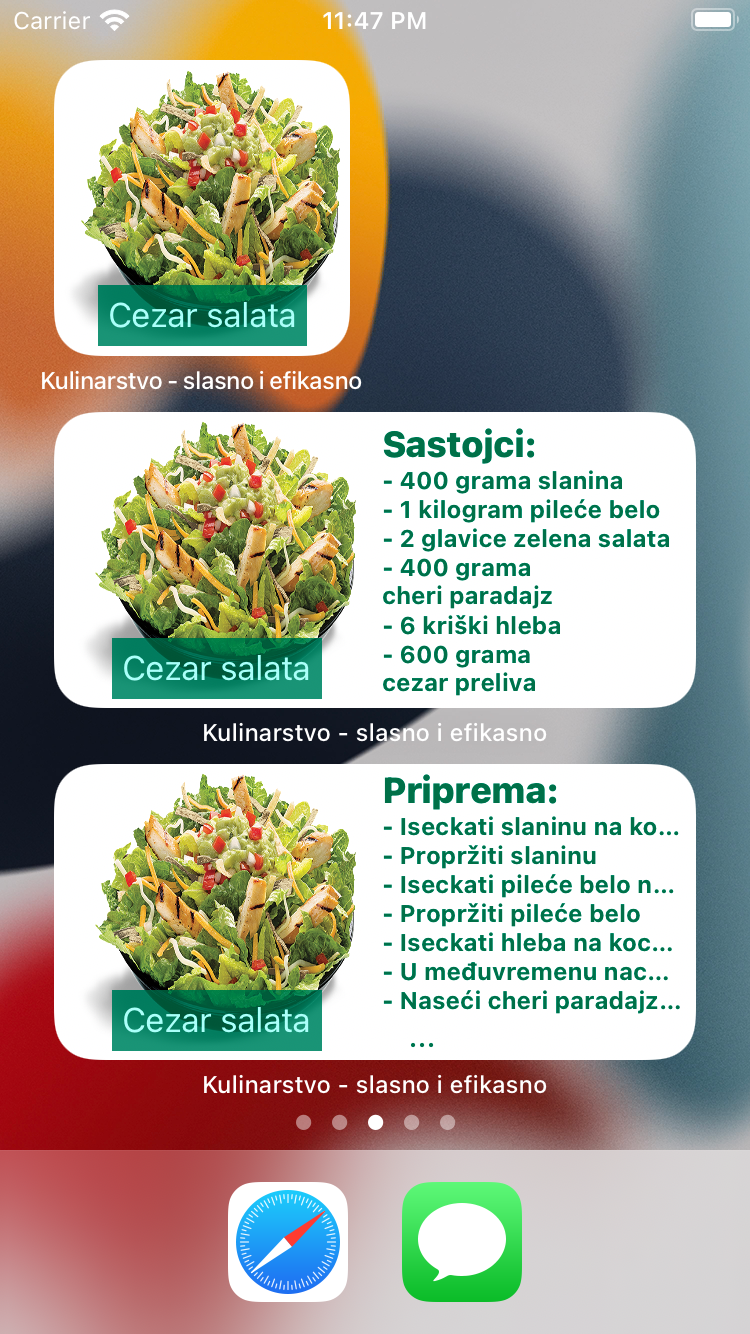
\includegraphics[width=0.475\textwidth]{images/simulators/view images/light - widgets 1-1.png} 
    \caption{\textit{Приказ виџета мале и средње величине --- iPhone 13 (лево) и iPhone SE (десно)}}
    \label{slika:приказ_виџета_1_1}
\end{figure}

\indent Први тип виџета у великој величини приказује рецепт са листама састојака и корака припреме, који су као код средњег виџета конфигурабилни и корисник може изабрати који ће од параметара бити примаран (приказан у дужој листи), уколико тај параметар испуњава услов --- дужина листе мора бити већа од шест елемената (уколико услов није испуњен, секундарни параметар ће бити приказан у дужој листи; док уколико ни секундарна листа не испуњава услов, обе листе ће бити приказане у кратком формату и слика рецепта ће заузети средишњи горњи део виџета). Велики виџет првог типа приказан је на слици \ref{slika:приказ_виџета_2_1}.

\begin{figure} [H]
    \centering
    \captionsetup{justification=centering}
    \includegraphics[width=0.475\textwidth]{images/simulators/view images/dark - widgets 1-2.png} 
    \hfill
    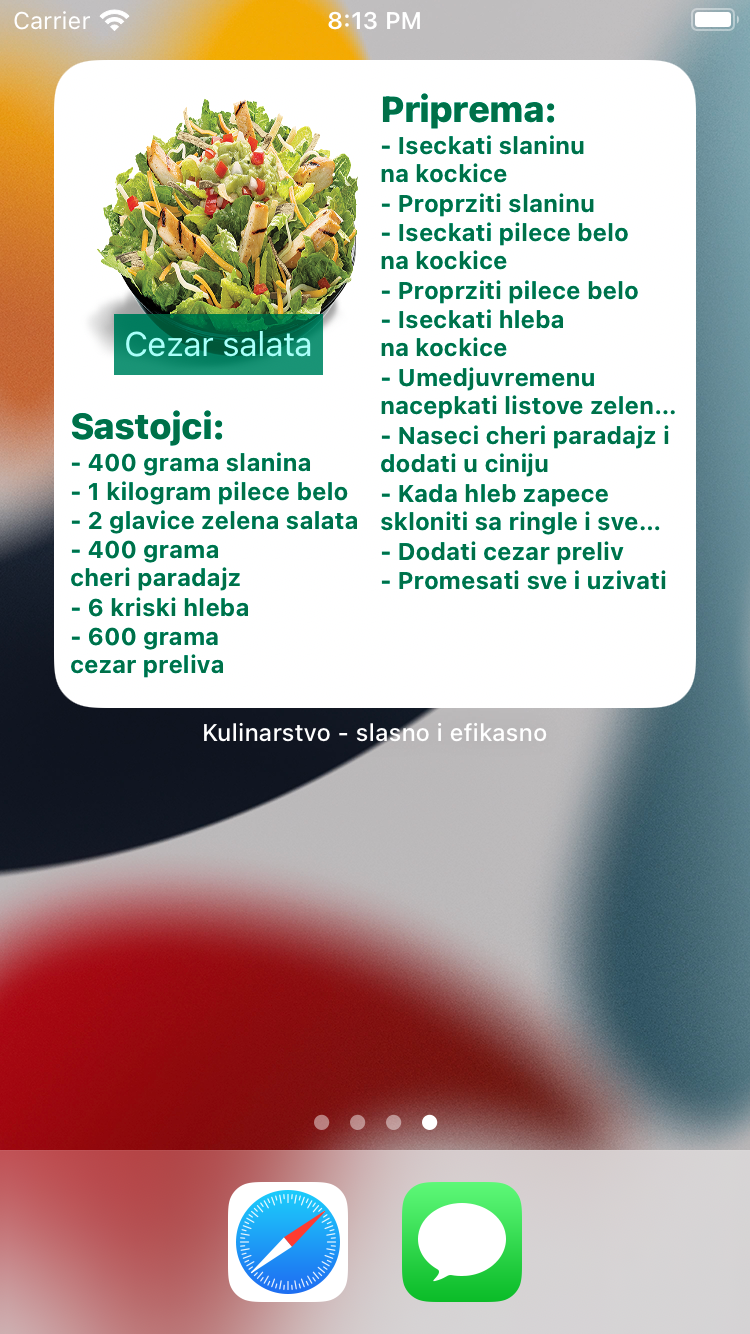
\includegraphics[width=0.475\textwidth]{images/simulators/view images/light - widgets 1-2.png} 
    \caption{\textit{Приказ првог виџета велике величине --- iPhone 13 (лево) и iPhone SE (десно)}}
    \label{slika:приказ_виџета_2_1}
\end{figure}

\indent Први тип виџета је конфигурабилан, односно корисник може мењати одређене параметре. Код малог виџета може променити рецепт који ће му бити приказан и изабрати неки од рецепата из своје листе омиљених рецепата. Средњи и велики виџет поред избора рецепта омогућавају и одабир примарног параметра (листа састојака или листа корака припреме). Изглед екрана приликом конфигурације средњег виџета приказан је на слици  \ref{slika:измена_виџета_1}.

\begin{figure} [H]
    \centering
    \captionsetup{justification=centering}
    
\includegraphics[width=0.475\textwidth]{images/simulators/view images/dark - change widget.png}
    \hfill
    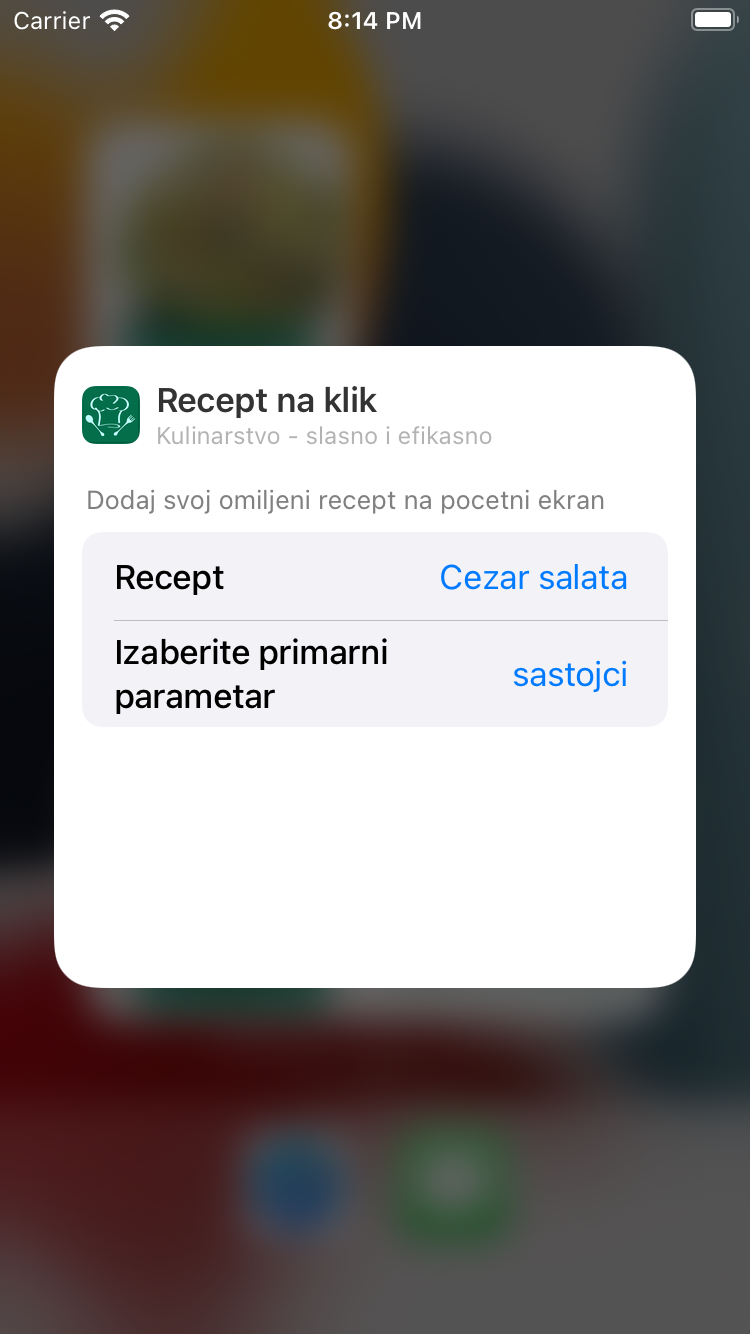
\includegraphics[width=0.475\textwidth]{images/simulators/view images/light - change widget.png} 
    \caption{\textit{Измена виџета --- iPhone 13 (лево) и iPhone SE (десно)}}
    \label{slika:измена_виџета_1}
\end{figure}

\indent Други тип виџета се разликује од првог по неколико карактеристика. Други тип је доступан само у великој величини, није га могуће конфигурисати и приказује четири рецепта. Рецепти који су приказани у овом типу виџета представљени су као скуп четири мала виџета првог типа, рецепти су насумично изабрани из корисникове листе омиљених рецепата, статички су конфигурисани и поновно се учитавају свака 24 сата и тако кориснику предлажу шта би могао да спрема тог дана. Приказ другог типа виџета може се видети на слици \ref{slika:приказ_виџета_3_1}.

\begin{figure} [H]
    \centering
    \captionsetup{justification=centering}
    \includegraphics[width=0.475\textwidth]{images/simulators/view images/dark - widgets 2-1.png} 
    \hfill
    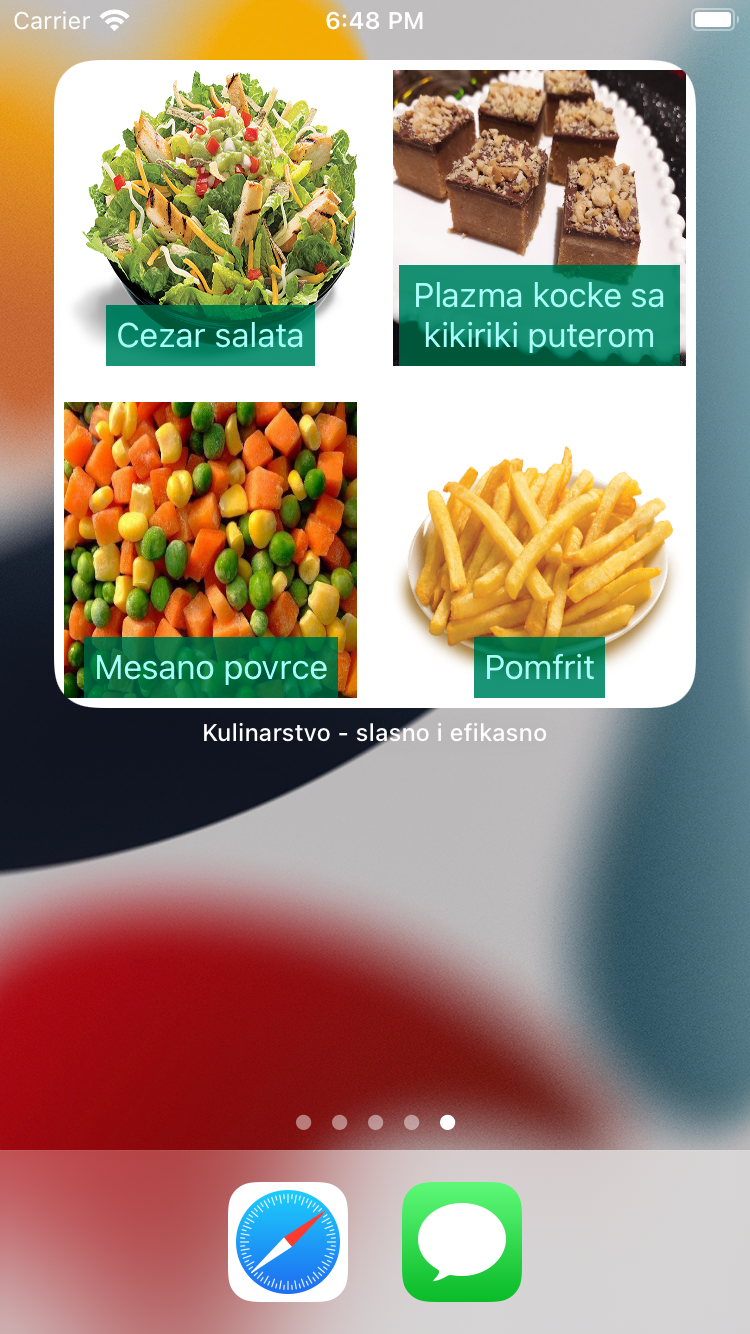
\includegraphics[width=0.475\textwidth]{images/simulators/view images/light - widgets 2-1.png}
    \caption{\textit{Приказ другог виџета велике величине --- iPhone 13 (лево) и iPhone SE (десно)}}
    \label{slika:приказ_виџета_3_1}
\end{figure}

% \subsection{Тестирање исправности апликације}
% \indent На слици \ref{slika:приказ_свих_рецепата} корисник може видети све рецепте који тренутно постоје унутар апликације. На слици \ref{slika:приказ_избора_категорије_претраге_рецепата} (лево) може се видети приказ рецепата који припадају категорији "Главно јело" док се на истој слици (десно) налазе рецепти који задовољавају тренутни услов претраге (име мора садржати стринг "М"). 

% % приказ свих рецепата
% \begin{figure} [H]
%     \centering
%     \captionsetup{justification=centering}
%     \includegraphics[width=0.475\textwidth]{images/simulators/testing images/general tab.png}
%     \caption{\textit{Приказ свих рецепата}}
%     \label{slika:приказ_свих_рецепата}
% \end{figure}

% % избор категорије
% % претрага
% \begin{figure} [H]
%     \centering
%     \captionsetup{justification=centering}
%     \includegraphics[width=0.475\textwidth]{images/simulators/testing images/choosen category.png}
%     \hfill
%     \includegraphics[width=0.475\textwidth]{images/simulators/testing images/search.png}
%     \caption{\textit{Приказ рецепата из категорије "Главно јело" (лево), претрага рецепта по стрингу "М" (десно)}}
%     \label{slika:приказ_избора_категорије_претраге_рецепата}
% \end{figure}

% \indent Слика \ref{slika:приказ_сортирања} приказује изглед почетног екрана када су рецепти сортирани по времену припреме (растуће на левој слици и опадајуће на десној). Када је корисник изабрао жељени рецепт, биће му приказан детаљан опис рецепта приказан на слици \ref{slika:детаљан_приказ_рецепта} (лево), а на истој слици десно је детаљан приказ тог рецепта за 6 особа уз пропратне промене (повећана количина потребних састојака и времена припреме). На слици \ref{slika:приказ_омиљених_рецепата} су приказана преостала два главна дела апликације, "Омиљени рецепти" лево и "Моји рецепти" десно.

% % сортирање
% \begin{figure} [H]
%     \centering
%     \captionsetup{justification=centering}
%     \includegraphics[width=0.475\textwidth]{images/simulators/testing images/sorting asc.png}
%     \hfill
%     \includegraphics[width=0.475\textwidth]{images/simulators/testing images/sorting desc.png}
%     \caption{\textit{Сортирање по времену припреме - растуће (лево) и опарајуће (десно)}}
%     \label{slika:приказ_сортирања}
% \end{figure}

% % детаљан приказ рецепта
% % манипулисање бројем особа
% \begin{figure} [H]
%     \centering
%     \captionsetup{justification=centering}
%     \includegraphics[width=0.475\textwidth]{images/simulators/testing images/detail recipe 4.png}
%     \hfill
%     \includegraphics[width=0.475\textwidth]{images/simulators/testing images/detail recipe 6.png}
%     \caption{\textit{Детаљан приказ рецепта}}
%     \label{slika:детаљан_приказ_рецепта}
% \end{figure}

% % приказ омилјених рецепата
% % приказ мојих рецепата
% \begin{figure} [H]
%     \centering
%     \captionsetup{justification=centering}
%     \includegraphics[width=0.475\textwidth]{images/simulators/testing images/favorite recipes.png}
%     \hfill
%     \includegraphics[width=0.475\textwidth]{images/simulators/testing images/my recipes.png}
%     \caption{\textit{Омиљени рецепти (лево) и моји рецепти (десно)}}
%     \label{slika:приказ_омиљених_рецепата}
% \end{figure}

% \indent У делу "Моји рецепти" корисник може додати нов рецепт. Креирање новог рецепта и његов детаљан приказ може се видети на слици \ref{slika:приказ_креирања_рецепта}. Уз додавање нових рецепата, тренутни корисник може изменити рецепте које је већ додао што је и приказано на слици \ref{slika:приказ_измењеног_рецепта}, лево се може видети измењено време припреме, број особа и додат нови састојак (2 прстохвата першуна), док је на десној слици приказан нови корак припреме (додати першун). Још једна могућност корисника је да обрише рецепт који је додао, приказано на слици \ref{slika:приказ_брисања_рецепта}, где се може видети да након брисања рецепта "Кокице" (лево), рецепт се више не налази у листи "Моји рецепти" (десно).

% % додавање новог рецепта
% \begin{figure} [H]
%     \centering
%     \captionsetup{justification=centering}
%     \includegraphics[width=0.475\textwidth]{images/simulators/testing images/create recipe.png}
%     \hfill
%     \includegraphics[width=0.475\textwidth]{images/simulators/testing images/new recipe.png}
%     \caption{\textit{Креирање новог рецепта}}
%     \label{slika:приказ_креирања_рецепта}
% \end{figure}

% % измена постојећег рецепта (основно, састојци, кораци)
% \begin{figure} [H]
%     \centering
%     \captionsetup{justification=centering}
%     \includegraphics[width=0.475\textwidth]{images/simulators/testing images/detail recipe change 1.png}
%     \hfill
%     \includegraphics[width=0.475\textwidth]{images/simulators/testing images/detail recipe change 2.png}
%     \caption{\textit{Измена рецепта}}
%     \label{slika:приказ_измењеног_рецепта}
% \end{figure}


% % брисање рецепта
% \begin{figure} [H]
%     \centering
%     \captionsetup{justification=centering}
%     \includegraphics[width=0.475\textwidth]{images/simulators/testing images/delete recipe.png}
%     \hfill
%     \includegraphics[width=0.475\textwidth]{images/simulators/testing images/deleted recipe.png}
%     \caption{\textit{Брисање рецепта}}
%     \label{slika:приказ_брисања_рецепта}
% \end{figure}

% % измена конфигурације виџета

% \indent Када корисник дода виџет средње величине на почетни екран подразумевани рецепт ће бити приказан, у овом случају то је "Омлет", док је примарни параметар "Састојци". Приказ додатог виџета на почетни екран може се видети на слици \ref{slika:приказ_конфигурације_виџета} (лево). Корисник може променити који ће рецепт бити приказан и изабрати неки из листе омиљених рецепата, приказано на истој слици у средини. Такође може променити и примарни параметар и поставити да то буде "Припрема", приказано на слици десно.

% \begin{figure} [H]
%     \centering
%     \captionsetup{justification=centering}
%     \includegraphics[width=0.3\textwidth]{images/simulators/testing images/added widget.png}
%     \hfill
%     \includegraphics[width=0.3\textwidth]{images/simulators/testing images/changed recipe widget.png}
%     \hfill
%     \includegraphics[width=0.3\textwidth]{images/simulators/testing images/changed parameter widget.png}
%     \caption{\textit{Конфигурација виџета}}
%     \label{slika:приказ_конфигурације_виџета}
% \end{figure}

\chapter{Закључак}

\indent У раду је описан програмски језик \textit{Swift}, његови основни и напредни концепти као и најважније особине. Опис језика је употпуњен конкретним примерима, којима су се постепено уводиле могућности које пружа овај програмски језик. Пример употребе програмског језика \textit{Swift} приказан је приликом израде \textit{iOS} апликације "Кулинарство --- сласно и ефикасно". 
\\
\indent Уз програмски језик \textit{Swift} у раду је представљена и могућност декларативног програмирања употребом радног окружења \textit{SwiftUI}. Конкретан пример употребе овог радног окружења приказан је приликом израде виџета који је имплементиран као додатак апликацији "Кулинарство --- сласно и ефикасно".
\\
\indent Описана је имплементација апликације "Кулинарство --- сласно и ефикасно" која има за циљ да крајњем кориснику пружи помоћ приликом одабира и припреме жељеног рецепта, уз приказ коришћене архитектуре и описа њених компоненти (модела, погледа и контролера). Апликација је у раду представљена и упоредним снимцима екрана два симулатора са различитим конфигурацијама уз описе њених делова, како би се приказала употреба апликације од стране корисника.
\\
\indent У току израде апликације показано је да је програмски језик \textit{Swift} безбедан и концизан, карактеристике које су у раду наведене као најважније. Радно окружење \textit{SwiftUI} је одличан начин примене декларативног програмирања и знатно скраћује време израде корисничког интерфејса апликације. Једна од запажених мана овог радног окружења приликом израде виџета је сама технологија која је веома млада и која се мења сваког дана, па се може наићи на потешкоће и нелогичности приликом њене употребе, које могу бити незгодне за превазилажење.
\\
\indent План за даље унапређење апликације је имплементација серверске стране апликације засноване на архитектуралном стилу репрезентативног преноса стања (енг. \textit{REpresentational State Transfer}, \textit{REST}) \cite{REST}. Поред тога биће додата функционалност креирања корисничких налога и пријављивања на исте употребом протокола \textit{OAuth 2.0} \cite{OAuth}.
% Даљи планови и могућа унапређења
% количина састојка као енум, Други тип виџета конфигурација категорије

\literatura

\chapter*{Биографија аутора}

\indent \textbf{Марко Вељковић} рођен је 27.02.1996. у Зајечару. Основну школу и информатички смер Зајечарске гимназије завршио је као носилац Вукове дипломе.
\\
\indent Смер информатика на Математичком факултету Универзитета у Београду уписао је 2015. године, а завршио септембра 2019. године са просечном оценом 8.53. Након тога је уписао мастер студије информатике на истом факултету.
\\
\indent У марту 2020. године почео је са праксом у компанији \textit{Teletrader} као јуниор \textit{iOS} програмер, где је након месец дана добио стално запослење. Тренутно ради у истом тиму као главни програмер на развоју и одржавању апликације \textit{StockMarkets} намењену уређајима \textit{iPad}, и усавршава своје знање у области развоја мобилних апликација за оперативне системе \textit{iOS}, \textit{iPadOS} и \textit{Android}.  

\end{document}
